% presentation
\documentclass{beamer}
\usetheme[height=7mm]{Rochester}
\usecolortheme{rose}

% handout

%\documentclass[handout]{beamer}
%\usepackage{pgfpages} \pgfpagesuselayout{8 on 1}[a4paper]

%\documentclass[mathserif]{article}
%\usepackage{beamerarticle}

\usepackage{amsmath}
\usepackage{comment}
\usepackage{amssymb,amsfonts}
\usepackage[T1]{fontenc}
\usepackage{lmodern}
\usepackage{tikz}
%\usepackage{simpsons}
\usepackage{marvosym}
\usepackage{color}
\usepackage{multirow}
\usepackage{pgffor}
\usepackage{pgfplots}
\usepackage[slide,algoruled,titlenumbered,vlined,noend,linesnumbered,]{algorithm2e}

\usefonttheme{structurebold}

\setbeamertemplate{footline}[frame number]
\setbeamertemplate{navigation symbols}{}
\setbeamerfont{smallverb}{size*={73}}
\usefonttheme[onlymath]{serif}
\setbeamertemplate{theorems}[numbered]
\newtheorem{construction}[theorem]{Construction}
\newtheorem{proposition}[theorem]{Proposition}

\AtBeginSection[] {
  \begin{frame}
    \frametitle{Content}
    \tableofcontents[currentsection]
  \end{frame}
  \addtocounter{framenumber}{-1}
}

\usetikzlibrary[shapes.arrows]
\usetikzlibrary{shapes.geometric}
\usetikzlibrary{backgrounds}
\usetikzlibrary{positioning}
\usetikzlibrary{calc}
\usetikzlibrary{intersections}
\usetikzlibrary{fadings}
\usetikzlibrary{decorations.footprints}
\usetikzlibrary{patterns}
\usetikzlibrary{shapes.callouts}
\usetikzlibrary{fit}
%handout

\providecommand{\abs}[1]{\lvert#1\rvert}

\tikzset{every picture/.style={line width=1pt,show background rectangle},background rectangle/.style={fill=blue!10,rounded corners=2ex}}

\newcommand{\Bob}[3]{ \begin{scope}[shift={(#1,#2)},scale=#3]
  \draw (0,0) circle (0.95 and 1);
  \fill (-0.3,-0.1) circle (0.1);
  \fill (+0.3,-0.1) circle (0.1);
  \draw (0.35,-0.5) arc (-70:-110: 1 and 0.4);
  \draw (-0.3,0.5) arc (-10:-80: 0.8 and 0.8);
  \draw (-0.5,0.8) arc (190:255: 2 and 1);
  \draw (-0.7,0.9) -- +(0.2,-0.09) -- +(0.25,0.2);
  \end{scope} }

\newcommand{\Alice}[3]{ \begin{scope}[shift={(#1,#2)},scale=#3]
  \draw (0,0) circle (0.95 and 1);
  \fill (-0.3,-0.1) circle (0.1);
  \fill (+0.3,-0.1) circle (0.1);
  \draw (0.35,-0.5) arc (-70:-110: 1 and 0.4);
  \draw (0.3,1.3) arc (20:-100: 1.4 and 1);
  \draw (0.5,1.3) arc (150:260: 1 and 1);
  \draw (0.41,1.3) circle (0.35);
  \end{scope} }

  \newcommand{\Evil}[3]{ \begin{scope}[shift={(#1,#2)},scale=#3]
    \draw (0,0) circle (0.95 and 1);
    \fill (-0.1,-0.1) -- +(-0.2,-0.1) -- +(-0.4,0.2); %eye
    \fill (0.1,-0.1) -- +(0.2,-0.1) -- +(0.4,0.2);
    \draw (0.35,-0.5) arc (-70:-110: 1 and 0.4);
    %\fill (0.3,-0.5) -- +(-0.1,-0.2) -- +(-0.2,-0.02);
    %\fill (-0.3,-0.5) -- +(0.1,-0.2) -- +(0.2,-0.02);
    \fill (0.3,0.7) -- +(0.5,0.4) -- +(0.4,-0.2); % horn
    \fill (-0.3,0.7) -- +(-0.5,0.4) -- +(-0.4,-0.2);
    %\draw (0.3,1.3) arc (20:-100: 1.4 and 1);
    %\draw (0.5,1.3) arc (150:260: 1 and 1);
    %\draw (0.41,1.3) circle (0.35);
    \end{scope} }

\newcommand{\Charlie}[3]{ \begin{scope}[shift={(#1,#2)},scale=#3]
    \draw (0,0) circle (0.95 and 1);
    \filldraw[fill=black!20] (-0.35,-0.1) circle (0.25);
    \filldraw[fill=black!20] (+0.35,-0.1) circle (0.25);
    %\draw (0.9,0.2) to [bend left] (-0.9,0.2);
    \draw (0.2,0) to [bend left] (-0.2,0);


    %\draw (0.3,0.7) to [bend right] (-0.3,0.7);
    %\draw (0.4,0.5) to [bend right] (-0.4,0.5);
    %\draw (0.35,-0.5) arc (-70:-110: 1 and 0.4);
    \draw (-0.7,-0.6) to [bend right] (0,-0.6) to [bend right] (0.7,-0.6) to [bend right]  (0,-0.5)  to [bend right]  cycle ;
    %\draw (0.3,1.3) arc (20:-100: 1.4 and 1);
    %\draw (0.5,1.3) arc (150:260: 1 and 1);
    %\draw (0.41,1.3) circle (0.35);
    \end{scope} }

\author{Yu Zhang}
\institute{Harbin Institute of Technology}
\date[Crypto'22A]{Cryptography, Autumn, 2022}

%% presentation
\documentclass{beamer}
\usetheme[height=7mm]{Rochester}
\usecolortheme{rose}

% handout

%\documentclass[handout]{beamer}
%\usepackage{pgfpages} \pgfpagesuselayout{8 on 1}[a4paper]

%\documentclass[mathserif]{article}
%\usepackage{beamerarticle}

\usepackage{amsmath}
\usepackage{comment}
\usepackage{amssymb,amsfonts}
\usepackage[T1]{fontenc}
\usepackage{lmodern}
\usepackage{tikz}
%\usepackage{simpsons}
\usepackage{marvosym}
\usepackage{color}
\usepackage{multirow}
\usepackage{pgffor}
\usepackage{pgfplots}
\usepackage[slide,algoruled,titlenumbered,vlined,noend,linesnumbered,]{algorithm2e}

\usefonttheme{structurebold}

\setbeamertemplate{footline}[frame number]
\setbeamertemplate{navigation symbols}{}
\setbeamerfont{smallverb}{size*={73}}
\usefonttheme[onlymath]{serif}
\setbeamertemplate{theorems}[numbered]
\newtheorem{construction}[theorem]{Construction}
\newtheorem{proposition}[theorem]{Proposition}

\AtBeginSection[] {
  \begin{frame}
    \frametitle{Content}
    \tableofcontents[currentsection]
  \end{frame}
  \addtocounter{framenumber}{-1}
}

\usetikzlibrary[shapes.arrows]
\usetikzlibrary{shapes.geometric}
\usetikzlibrary{backgrounds}
\usetikzlibrary{positioning}
\usetikzlibrary{calc}
\usetikzlibrary{intersections}
\usetikzlibrary{fadings}
\usetikzlibrary{decorations.footprints}
\usetikzlibrary{patterns}
\usetikzlibrary{shapes.callouts}
\usetikzlibrary{fit}
%handout

\providecommand{\abs}[1]{\lvert#1\rvert}

\tikzset{every picture/.style={line width=1pt,show background rectangle},background rectangle/.style={fill=blue!10,rounded corners=2ex}}

\newcommand{\Bob}[3]{ \begin{scope}[shift={(#1,#2)},scale=#3]
  \draw (0,0) circle (0.95 and 1);
  \fill (-0.3,-0.1) circle (0.1);
  \fill (+0.3,-0.1) circle (0.1);
  \draw (0.35,-0.5) arc (-70:-110: 1 and 0.4);
  \draw (-0.3,0.5) arc (-10:-80: 0.8 and 0.8);
  \draw (-0.5,0.8) arc (190:255: 2 and 1);
  \draw (-0.7,0.9) -- +(0.2,-0.09) -- +(0.25,0.2);
  \end{scope} }

\newcommand{\Alice}[3]{ \begin{scope}[shift={(#1,#2)},scale=#3]
  \draw (0,0) circle (0.95 and 1);
  \fill (-0.3,-0.1) circle (0.1);
  \fill (+0.3,-0.1) circle (0.1);
  \draw (0.35,-0.5) arc (-70:-110: 1 and 0.4);
  \draw (0.3,1.3) arc (20:-100: 1.4 and 1);
  \draw (0.5,1.3) arc (150:260: 1 and 1);
  \draw (0.41,1.3) circle (0.35);
  \end{scope} }

  \newcommand{\Evil}[3]{ \begin{scope}[shift={(#1,#2)},scale=#3]
    \draw (0,0) circle (0.95 and 1);
    \fill (-0.1,-0.1) -- +(-0.2,-0.1) -- +(-0.4,0.2); %eye
    \fill (0.1,-0.1) -- +(0.2,-0.1) -- +(0.4,0.2);
    \draw (0.35,-0.5) arc (-70:-110: 1 and 0.4);
    %\fill (0.3,-0.5) -- +(-0.1,-0.2) -- +(-0.2,-0.02);
    %\fill (-0.3,-0.5) -- +(0.1,-0.2) -- +(0.2,-0.02);
    \fill (0.3,0.7) -- +(0.5,0.4) -- +(0.4,-0.2); % horn
    \fill (-0.3,0.7) -- +(-0.5,0.4) -- +(-0.4,-0.2);
    %\draw (0.3,1.3) arc (20:-100: 1.4 and 1);
    %\draw (0.5,1.3) arc (150:260: 1 and 1);
    %\draw (0.41,1.3) circle (0.35);
    \end{scope} }

\newcommand{\Charlie}[3]{ \begin{scope}[shift={(#1,#2)},scale=#3]
    \draw (0,0) circle (0.95 and 1);
    \filldraw[fill=black!20] (-0.35,-0.1) circle (0.25);
    \filldraw[fill=black!20] (+0.35,-0.1) circle (0.25);
    %\draw (0.9,0.2) to [bend left] (-0.9,0.2);
    \draw (0.2,0) to [bend left] (-0.2,0);


    %\draw (0.3,0.7) to [bend right] (-0.3,0.7);
    %\draw (0.4,0.5) to [bend right] (-0.4,0.5);
    %\draw (0.35,-0.5) arc (-70:-110: 1 and 0.4);
    \draw (-0.7,-0.6) to [bend right] (0,-0.6) to [bend right] (0.7,-0.6) to [bend right]  (0,-0.5)  to [bend right]  cycle ;
    %\draw (0.3,1.3) arc (20:-100: 1.4 and 1);
    %\draw (0.5,1.3) arc (150:260: 1 and 1);
    %\draw (0.41,1.3) circle (0.35);
    \end{scope} }

\author{Yu Zhang}
\institute{Harbin Institute of Technology}
\date[Crypto'22A]{Cryptography, Autumn, 2022}

%\input{1introduction.tex}
%\input{2perfectlysecret.tex}
%\input{3privatekey.tex}


\title{Introduction}

\begin{document}
\maketitle
\begin{frame}
\frametitle{Outline}
\tableofcontents
\end{frame}
\section{Cryptography and Modern Cryptography}
\begin{frame}\frametitle{What is Cryptography?}
\begin{itemize}
\item \textbf{Cryptography}: from Greek \emph{krypt\'os}, ``hidden, secret''; and \emph{gr\'{a}phin}, ``writing''
\item \textbf{Cryptography}: the art of writing or solving codes.\\ (Concise oxford dictionary 2006)
\item \textbf{Codes}: a system of prearranged signals, especially used to ensure secrecy in transmitting messages. \\ (\emph{code word} in cryptography)
\item \textbf{1980s}: from Classic to Modern; from Military to Everyone
\item \textbf{Modern cryptography}: the scientific study of mathematical techniques for securing digital information, systems, and distributed computations against adversarial attacks
\end{itemize}
\end{frame}
\begin{frame}\frametitle{What is cryptography? [xkcd:504]}
\begin{figure}
\begin{center}
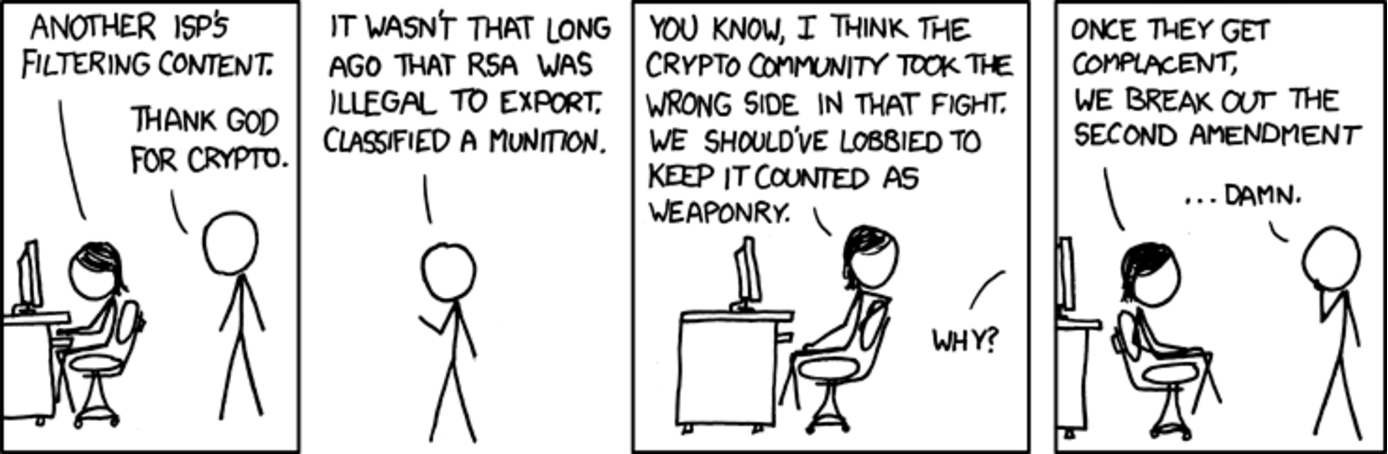
\includegraphics[width=100mm]{pic/legal} 
\end{center}
\end{figure}
\end{frame}
\section{The Setting of Private-Key Encryption}
\begin{frame}\frametitle{Private-Key Encryption}
\begin{itemize}
\item \textbf{Goal}: to construct \textbf{ciphers} (encryption schemes) for providing secret communication between two parties sharing \textbf{private-key} (the symmetric-key) in advance
\item \textbf{Implicit assumption}: there is some way of initially sharing a key in a secret manner
\item \textbf{Disk encryption}: the same user at different points in time
\end{itemize}
\end{frame}
\begin{frame}\frametitle{Alice, Bob  [xkcd:1323]}
Changing the names would be easier, but if you're not comfortable lying, try only making friends with people named Alice, Bob, Carol, etc.
\begin{figure}
\begin{center}
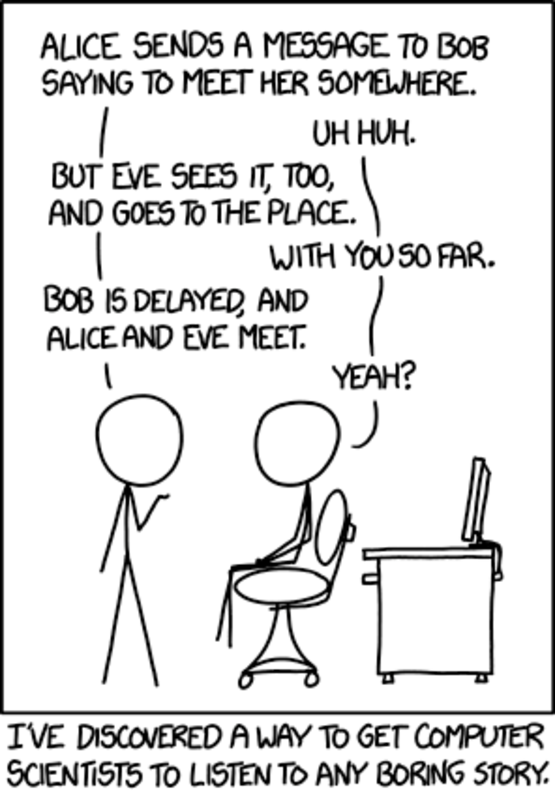
\includegraphics[width=45mm]{pic/alice-bob} 
\end{center}
\end{figure}
\end{frame}
\begin{frame}\frametitle{The Syntax of Encryption}
\begin{figure}
\begin{center}
\begin{tikzpicture}
\node (sender) [minimum size=1cm] {}; \Alice{0}{0}{0.4};
\node (bart) [below of = sender, node distance = 0.7cm] {Alice};
\node (enc) [draw, right of = sender, rounded corners=1ex,node distance = 2cm] {$\mathsf{Enc}$};
\node (k1) [above of = enc, node distance = 1cm] {$k$};
\node (c) [right of = enc, node distance = 2cm] {$c$};
\node (gen) [draw, above of = c, rounded corners=1ex,node distance = 1cm] {$\mathsf{Gen}$};
\node (adv) [below of = c, node distance = 1cm, minimum size=1cm] {}; \Evil{4cm}{-1cm}{0.4};
\node (burns) [below of = adv, node distance = 0.7cm] {Adversary};
\node (dec) [draw, right of = c, rounded corners=1ex,node distance = 2cm] {$\mathsf{Dec}$};
\node (k2) [above of = dec, node distance = 1cm] {$k$};
\node (receiver) [right of = dec, node distance = 2cm, minimum size=1cm] {}; \Bob{8cm}{0}{0.4};
\node (lisa) [below of = receiver, node distance = 0.7cm] {Bob};
\draw[-latex] (sender) -- (enc) node [midway, above] {$m$};
\draw (enc) -- (c); \draw[-latex] (c) -- (dec);
\draw[-latex] (dec) -- (receiver) node [midway, above] {$m$};
\draw[-latex] (k1) -- (enc);
\draw[-latex] (gen) -- (k1);
\draw[-latex] (gen) -- (k2);								
\draw[-latex] (k2) -- (dec);		
\end{tikzpicture}
\end{center}
\end{figure}
\begin{itemize}
\item key $k \in \mathcal{K}$, plaintext (or message) $m \in \mathcal{M}$, ciphertext $c \in \mathcal{C}$
\item \textbf{Key-generation} algorithm~$k \gets \mathsf{Gen}$
\item \textbf{Encryption} algorithm~$c:= \mathsf{Enc}_k(m)$
\item \textbf{Decryption} algorithm~$m:= \mathsf{Dec}_k(c)$
\item \textbf{Encryption scheme}: $\Pi = (\mathsf{Gen}, \mathsf{Enc}, \mathsf{Dec})$
\item \textbf{Basic correctness requirement}: $\mathsf{Dec}_k(\mathsf{Enc}_k(m)) = m$
\end{itemize}
\end{frame}
\begin{frame}\frametitle{Securing Key vs Obscuring Algorithm}
\begin{itemize}
\item Easier to maintain secrecy of a short key
\item In case the key is exposed, easier for the honest parties to change the key
\item In case many pairs of people, easier to use the same algorithm, but different keys
\end{itemize}
\begin{alertblock}{Kerckhoffs's principle}
\begin{quote}
The cipher method must not be required to be secret, and it must be able to fall into the hands of the enemy without inconvenience.
\end{quote}	
\end{alertblock}
\begin{alertblock}{Shannon's maxim}
	\begin{quote}
		The enemy knows the system.
	\end{quote}	
\end{alertblock}
\end{frame}
\begin{frame}\frametitle{Why ``Open Cryptographic Design''}
\begin{itemize}
\item Published designs undergo public scrutiny are to be stronger
\item Better for security flaws to be revealed by ``ethical hackers''
\item Reverse engineering of the code (or leakage by industrial espionage) poses a serious threat to security
\item Enable the establishment of standards.
\end{itemize}
\begin{exampleblock}{Dual EC: A Standardized Back Door}
	``Dual EC was standardized by NIST, ANSI, and ISO among other algorithms to generate pseudorandom numbers.'' ``The Snowden revelations, and in particular reports on Project Bullrun and the SIGINT Enabling Project, have indicated that Dual EC was part of a systematic effort by NSA to subvert standards.'' ``Reuters reported that NSA paid RSA ``\$10 million in a deal that set [Dual EC] as the preferred, or default, method for number generation in the BSafe software.''''	
\end{exampleblock}
\end{frame}
\begin{frame}\frametitle{Attack Scenarios}	
\begin{itemize}
\item \textbf{Ciphertext-only}: the adversary just observes ciphertext
\item \textbf{Known-plaintext}: the adversary learns pairs of plaintexts/ciphertexts under the same key
\item \textbf{Chosen-plaintext}: the adversary has the ability to obtain the encryption of plaintexts of its choice
\item \textbf{Chosen-ciphertext}: the adversary has the ability to obtain the decryption of \textbf{other} ciphertexts of its choice
\item \textbf{Passive attack}: COA KPA
\begin{itemize}
\item because not all ciphertext are confidential
\end{itemize}
\item \textbf{Active attack}: CPA CCA
\begin{itemize}
\item when to encrypt/decrypt whatever an adversary wishes?
\end{itemize}
\end{itemize}	
\end{frame}
\section{Historical Ciphers and Their Cryptanalysis}
\begin{comment}
	\begin{frame}\frametitle{Why We Learn Broken Ciphers?}
	\begin{itemize}
	\item To understand the weaknesses of an ``ad-hoc'' approach
	\item To learn that ``simple'' approaches are unlikely to succeed
	\item To feel that ``we are smart enough to do some crypt-analyzing''
	\end{itemize}
	\end{frame}
\end{comment}

\begin{frame}[fragile]\frametitle{Caesar's Cipher}
\begin{quote}
If he had anything confidential to say, he wrote it in cipher, that is, by so changing the order of the letters of the alphabet, that not a word could be made out. If anyone wishes to \alert{decipher} these, and get at their meaning, he must \alert{substitute the fourth letter of the alphabet, namely D, for A}, and so with the others

\rightline{--Suetonius,``Life of Julius Caesar''}
\end{quote}
\begin{itemize}
	\item $\mathsf{Enc}(m)=m+3\mod 26$ \footnote{In fact the quote indicates that decryption involved rotating letters of the alphabet forward 3 positions, $\mathsf{Dec}(c)=c+3\mod 26$}
	\item \textbf{Weakness}: ? %\alert{What is the key?}
\end{itemize}
\begin{exampleblock}{Example}
\verb|begintheattacknow|
%\verb|EHJLQWKHDWWDFNQRZ|
\end{exampleblock}
\end{frame}
\begin{frame}[fragile]\frametitle{Shift Cipher}
\begin{itemize}
\item $\mathsf{Enc}_k(m)=m+k\mod 26$
\item $\mathsf{Dec}_k(c)=c-k\mod 26$
\item \textbf{Weakness}: ? %Fragile under \textbf{Brute-force attack} (exhaustive search)
\end{itemize}
\begin{exampleblock}{Example: Decipher the string}	
\verb|EHJLQWKHDWWDFNQRZ|
\end{exampleblock}
\begin{alertblock}{Sufficient Key Space Principle}
Any secure encryption scheme must have a key space that is not vulnerable to exhaustive search.\footnote{If the plaintext space is larger than the key space.}
\end{alertblock}
\end{frame}
\begin{frame}\frametitle{Index of Coincidence (IC) Method (to find $k$)}
\textbf{How to automatically determine that the deciphered text makes sense?}

\textbf{Index of Coincidence (IC)}: the probability that two randomly selected letters (pick-then-return) will be identical.

Let $p_i$ denote the probability of $i$th letter in English text.
\[I \overset{\text{def}}{=}\sum_{i=0}^{25} p_i^2 \]
\begin{exampleblock}{Example}
What's the IC of `apple'?
\end{exampleblock}

For a long English text, the IC is $\approx 0.065$.
For $j = 0, 1, \dotsc , 25$, $q_j$ is the probability of $j$th letter in the ciphertext.
\[I_j \overset{\text{def}}{=}\sum_{i=0}^{25} p_i \cdot q_{i+j}\]
\alert{Q: For shift cipher, if $j = k$, then $I_j \approx$ ?}
\end{frame}

\begin{frame}[fragile]\frametitle{Mono-Alphabetic Substitution}
\begin{itemize}
\item \textbf{Idea}: To map each character to a different one in an arbitrary manner
\item \textbf{Strength}: Key space is large $\approx 2^{88}$. \alert{Q: how to count?}
\item \textbf{Weakness}: ? %The mapping of each letter is fixed
\end{itemize}
\begin{exampleblock}{Example}
\verb|abcdefghijklmnopqrstuvwxyz|\\
\verb|XEUADNBKVMROCQFSYHWGLZIJPT|

Plaintext: \verb|tellhimaboutme|\\
Ciphertext: \verb|??????????????|
\end{exampleblock}
\end{frame}
\begin{frame}[fragile]\frametitle{Attack with Statistical Patterns}
\begin{enumerate}
\item Tabulate the frequency of letters in the ciphertext
\item Compare it to those in English text
\item Guess the most frequent letter corresponds to \verb|e|, and so on
\item Choose the plaintext that does ``make sense'' (Not trivial)
\end{enumerate}
\begin{table}
\begin{center}
\caption{Average letter frequencies for English-language text}
\begin{tabular}{|cc|cc|cc|cc|cc|} \hline
e & 12.7\% & t & 9.1\% & a & 8.2\% & o & 7.5\% & i & 7.0\%\\
n & 6.7\% & \_ & 6.4\% & s & 6.3\% & h & 6.1\% & r & 6.0\%\\
d & 4.3\% & l & 4.0\% & c & 2.8\% & u & 2.8\% & m & 2.4\%\\
w & 2.4\% & f & 2.2\% & g & 2.0\% & y & 2.0\% & p & 1.9\%\\
b & 1.5\% & v & 1.0\% & k & 0.8\% & j & 0.2\% & x & 0.2\%\\
q & 0.1\% & z & 0.1\% & & & & & &\\ \hline
\end{tabular}
\end{center}
\end{table}
\end{frame}
\begin{frame}[fragile]\frametitle{Example of Frequency Analysis (Ciphertext)}
\begin{verbatim}
LIVITCSWPIYVEWHEVSRIQMXLEYVEOIEWHRXEXIPFEMVEWHKVS
TYLXZIXLIKIIXPIJVSZEYPERRGERIMWQLMGLMXQERIWGPSRIH
MXQEREKIETXMJTPRGEVEKEITREWHEXXLEXXMZITWAWSQWXSWE
XTVEPMRXRSJGSTVRIEYVIEXCVMUIMWERGMIWXMJMGCSMWXSJO
MIQXLIVIQIVIXQSVSTWHKPEGARCSXRWIEVSWIIBXVIZMXFSJX
LIKEGAEWHEPSWYSWIWIEVXLISXLIVXLIRGEPIRQIVIIBGIIHM
WYPFLEVHEWHYPSRRFQMXLEPPXLIECCIEVEWGISJKTVWMRLIHY
SPHXLIQIMYLXSJXLIMWRIGXQEROIVFVIZEVAEKPIEWHXEAMWY
EPPXLMWYRMWXSGSWRMHIVEXMSWMGSTPHLEVHPFKPEZINTCMXI
VJSVLMRSCMWMSWVIRCIGXMWYMX
\end{verbatim}
\end{frame}
\begin{frame}[fragile]\frametitle{Example of Frequency Analysis (Analysis)}
Count and Guess, Trial and Error.
\begin{table}
\begin{center}
\caption{Analysis Steps}
\begin{tabular}{|r|l|} \hline
Ciphertext & Plaintext \\ \hline
\alert{I}   & \alert{e} \\
\alert{XLI} & \alert{the} \\
\alert{E} & \alert{a} \\
\alert{R}tate & \alert{s}tate \\
atthatt\alert{MZ}e & atthatt\alert{im}e \\
he\alert{V}e & he\alert{r}e \\
remar\alert{A} & remar\alert{k} \\ \hline
\end{tabular}
\end{center}
\end{table}
\end{frame}
\begin{frame}[fragile]\frametitle{Example of Frequency Analysis (Plaintext)}
\begin{quote}
Hereupon Legrand arose, with a grave and stately air, and brought me the beetle
from a glass case in which it was enclosed. It was a beautiful scarabaeus, and, at
that time, unknown to naturalists -- of course a great prize in a scientific point
of view. There were two round black spots near one extremity of the back, and a
long one near the other. The scales were exceedingly hard and glossy, with all the
appearance of burnished gold. The weight of the insect was very remarkable, and,
taking all things into consideration, I could hardly blame Jupiter for his opinion
respecting it.

\rightline{--Edgar Allan Poe's ``The Gold-Bug''}
\end{quote}
\end{frame}

\begin{frame}[fragile]\frametitle{Vigen\`{e}re (poly-alphabetic shift) Cipher}
\begin{itemize}
\item \textbf{Idea}: To ``smooth out'' the distribution in the ciphertext by mapping different instances of the same letter in the plaintext to different ones in the ciphertext
\item \textbf{Encryption}: $c_i=m_i+k_{[i\bmod t]}$, $t$ is the length (period) of $k$
\item \textbf{Cryptanalysis}: Need find $t$; if $t$ is known, need know whether the decryption ``makes sense'', but brute force ($26^t$) is infeasible for $t > 15$
\end{itemize}
\begin{exampleblock}{Example (Key is `cafe')}
\begin{description}[Ciphertext]
\item[Plaintext]  \verb|tellhimaboutme| \\
\item[Key]        \verb|cafecafecafeca| \\
\item[Ciphertext] \verb|??????????????| %\verb|WFRQKJSFEPAYPF|
\end{description}
\end{exampleblock}
\end{frame}
\begin{frame}[fragile]\frametitle{Kasiski's Method (to find $t$)}
\begin{itemize}
\item To identify repeated patterns of length 2 or 3
\item The distance between such appearances is a multiple of $t$
\item $t$ is the greatest common divisor of all the distances
\end{itemize}
\begin{exampleblock}{Example (Key is `beads')}
\begin{semiverbatim}
themanandthewomanretrievedtheletterfromthepostoffice
beadsbeadsbeadsbeadsbeadsbeansdeadsbeadsbeadsbeadbea
VMFQTPFOH\alert{MJJ}XSFCSSIMTNFZXFYISEIYUIKHWPQ\alert{MJJ}QSLVTGJKGF
\end{semiverbatim}
\end{exampleblock}
\end{frame}
\begin{frame}\frametitle{Index of Coincidence (IC) Method (to find $t$)}
For $\tau = 1, 2, \dotsc$, $q_i$ is the probability of $i$th letter in $c_1, c_{1+\tau}, c_{1+2\tau}, \dotsc$, IC is
\[I_\tau \overset{\text{def}}{=}\sum_{i=0}^{25} q_i^2\]
\alert{If $\tau = t$, then $I_\tau \approx ?$} ; otherwise $q_i \approx \frac{1}{26}$ and
\[I_\tau \approx \sum_{i=0}^{25} \left(\frac{1}{26}\right)^2 \approx 0.038\]
Then reuse IC method to find $k_i$.
\begin{alertblock}{Arbitrary Adversary Principle}
Security must be guaranteed for any adversary within the class of adversaries having the specified power
\end{alertblock}
\end{frame}
\begin{frame}\frametitle{Cryptanalytic Attacks (homework assignment)}
\begin{itemize}
\item Under COA, the requirement for ciphertext related to the size of the key space.  Vig\`{e}nere > mono-alphabetic sub. > shift
\item Under KPA, trivially broken.
\end{itemize}
\begin{alertblock}{Lessons learned}
\begin{itemize}
\item Sufficient key space principle
\item Designing secure cipher is a hard task
\item Complexity does not imply security (then what does?)
\item Arbitrary adversary principle
\end{itemize}
\end{alertblock}
\end{frame}
\section{The Basic Principles of Modern Cryptography}
\begin{frame}\frametitle{Three Main Principles of Modern Cryptography}
\begin{enumerate}
\item The formulation of a rigorous \textbf{definition} of security / threat model
\item When the security of a cipher relies on an unproven \textbf{assumption}, this assumption must be precisely stated and be as minimal as possible
\item Cipher should be accompanied by a rigorous \textbf{proof} of security with the above definition and the above assumption
\end{enumerate}
\end{frame}
\begin{frame}\frametitle{Why Principle 1 -- Formulation of Exact Definitions}
\begin{exampleblock}{Q: how would you formalize the security for private-key encryption?}
\begin{enumerate}
\item \emph{No adversary can find the secret key when given a ciphertext.}\\
$\mathsf{Enc}_k(m)=m$
\item \emph{No adversary can find the plaintext that corresponds to the ciphertext.}\\
$\mathsf{Enc}_k(m)=m_{0}\| \mathsf{AES}_k(m)$
\item \emph{No adversary can determine any character of the plaintext that corresponds to the ciphertext.}\\
$m=1000$, someone can learn $ 800 < m < 1200$
\item \emph{No adversary can derive any meaningful information about the plaintext from the ciphertext.}\\
Could you define so-called `meaningful'?
\end{enumerate}
\emph{\alert{Definitions of security should suffice for all potential applications.}}
\end{exampleblock}
\end{frame}
\begin{frame}\frametitle{Why Principle 1 -- How to define}
%\begin{exampleblock}{General Form}
%A cryptographic scheme for a given \textbf{task} is secure if no adversary of a specified \textbf{power} can achieve a specified \textbf{break}
%\end{exampleblock}

How To Define Security -- Lesson From Alan Turing
\begin{itemize}
\item What's computation?\footnote{Q: Any ``mathematical proof that there exist well-defined problems that computers cannot solve''? A: Halting Problem in computability theory}
\begin{enumerate}
\item A direct appeal to \textbf{intuition}
\item A \textbf{proof of the equivalence} of two definitions\\ (The new one has a greater intuitive appeal)
\item Giving \textbf{examples} solved using a definition
\end{enumerate}
\item Additional method for security: \textbf{Test of time}
\end{itemize}
\end{frame}	
\begin{frame}\frametitle{Principle 2 -- Reliance on Precise Assumptions}
Most cryptographic constructions \textbf{cannot be proven secure unconditionally}
\begin{itemize}
	\item \textbf{Why?} 
	\begin{enumerate}
		\item Validation of the assumption
		\item Comparison of schemes
		\item Facilitation of proofs of security
	\end{enumerate}
	\textbf{The construction is secure if the assumption is true.}
	\item \textbf{How?} 
	\begin{enumerate}
		\item old, so well tested
		\item simple and lower-level, so easy to study, refute \& correct
	\end{enumerate}
\end{itemize}
\end{frame}
\begin{frame}\frametitle{Principle 3 -- Rigorous Proofs of Security}
\begin{itemize}
\item \textbf{Why?} Proofs are more desirable in computer security than in other fields.
\item \textbf{The reductionist approach}: 
\begin{theorem}	Given that Assumption X is true, Construction Y is secure according to the given definition.
\end{theorem}
\begin{proof} Reduce the problem given by X to the problem of breaking Y.
\end{proof}
\item \textbf{Ad-hoc approaches}: for those who need a ``quick and dirty'' solution, or who are just simply unaware.
\end{itemize}
\end{frame}
\begin{frame}\frametitle{Summary}
\begin{itemize}
\item Cryptography secures information, transactions and computations
\item Kerckhoffs's principle \& Open cryptographic design
\item Caesar's, shift, Mono-Alphabetic sub., Vigen\`{e}re
\item Brute force, letter frequency, Kasiski's, IC
\item Sufficient key space principle
\item Arbitrary adversary principle
\item Rigorously proven security
\end{itemize}
\end{frame}
\end{document}


%% presentation
\documentclass{beamer}
\usetheme[height=7mm]{Rochester}
\usecolortheme{rose}

% handout

%\documentclass[handout]{beamer}
%\usepackage{pgfpages} \pgfpagesuselayout{8 on 1}[a4paper]

%\documentclass[mathserif]{article}
%\usepackage{beamerarticle}

\usepackage{amsmath}
\usepackage{comment}
\usepackage{amssymb,amsfonts}
\usepackage[T1]{fontenc}
\usepackage{lmodern}
\usepackage{tikz}
%\usepackage{simpsons}
\usepackage{marvosym}
\usepackage{color}
\usepackage{multirow}
\usepackage{pgffor}
\usepackage{pgfplots}
\usepackage[slide,algoruled,titlenumbered,vlined,noend,linesnumbered,]{algorithm2e}

\usefonttheme{structurebold}

\setbeamertemplate{footline}[frame number]
\setbeamertemplate{navigation symbols}{}
\setbeamerfont{smallverb}{size*={73}}
\usefonttheme[onlymath]{serif}
\setbeamertemplate{theorems}[numbered]
\newtheorem{construction}[theorem]{Construction}
\newtheorem{proposition}[theorem]{Proposition}

\AtBeginSection[] {
  \begin{frame}
    \frametitle{Content}
    \tableofcontents[currentsection]
  \end{frame}
  \addtocounter{framenumber}{-1}
}

\usetikzlibrary[shapes.arrows]
\usetikzlibrary{shapes.geometric}
\usetikzlibrary{backgrounds}
\usetikzlibrary{positioning}
\usetikzlibrary{calc}
\usetikzlibrary{intersections}
\usetikzlibrary{fadings}
\usetikzlibrary{decorations.footprints}
\usetikzlibrary{patterns}
\usetikzlibrary{shapes.callouts}
\usetikzlibrary{fit}
%handout

\providecommand{\abs}[1]{\lvert#1\rvert}

\tikzset{every picture/.style={line width=1pt,show background rectangle},background rectangle/.style={fill=blue!10,rounded corners=2ex}}

\newcommand{\Bob}[3]{ \begin{scope}[shift={(#1,#2)},scale=#3]
  \draw (0,0) circle (0.95 and 1);
  \fill (-0.3,-0.1) circle (0.1);
  \fill (+0.3,-0.1) circle (0.1);
  \draw (0.35,-0.5) arc (-70:-110: 1 and 0.4);
  \draw (-0.3,0.5) arc (-10:-80: 0.8 and 0.8);
  \draw (-0.5,0.8) arc (190:255: 2 and 1);
  \draw (-0.7,0.9) -- +(0.2,-0.09) -- +(0.25,0.2);
  \end{scope} }

\newcommand{\Alice}[3]{ \begin{scope}[shift={(#1,#2)},scale=#3]
  \draw (0,0) circle (0.95 and 1);
  \fill (-0.3,-0.1) circle (0.1);
  \fill (+0.3,-0.1) circle (0.1);
  \draw (0.35,-0.5) arc (-70:-110: 1 and 0.4);
  \draw (0.3,1.3) arc (20:-100: 1.4 and 1);
  \draw (0.5,1.3) arc (150:260: 1 and 1);
  \draw (0.41,1.3) circle (0.35);
  \end{scope} }

  \newcommand{\Evil}[3]{ \begin{scope}[shift={(#1,#2)},scale=#3]
    \draw (0,0) circle (0.95 and 1);
    \fill (-0.1,-0.1) -- +(-0.2,-0.1) -- +(-0.4,0.2); %eye
    \fill (0.1,-0.1) -- +(0.2,-0.1) -- +(0.4,0.2);
    \draw (0.35,-0.5) arc (-70:-110: 1 and 0.4);
    %\fill (0.3,-0.5) -- +(-0.1,-0.2) -- +(-0.2,-0.02);
    %\fill (-0.3,-0.5) -- +(0.1,-0.2) -- +(0.2,-0.02);
    \fill (0.3,0.7) -- +(0.5,0.4) -- +(0.4,-0.2); % horn
    \fill (-0.3,0.7) -- +(-0.5,0.4) -- +(-0.4,-0.2);
    %\draw (0.3,1.3) arc (20:-100: 1.4 and 1);
    %\draw (0.5,1.3) arc (150:260: 1 and 1);
    %\draw (0.41,1.3) circle (0.35);
    \end{scope} }

\newcommand{\Charlie}[3]{ \begin{scope}[shift={(#1,#2)},scale=#3]
    \draw (0,0) circle (0.95 and 1);
    \filldraw[fill=black!20] (-0.35,-0.1) circle (0.25);
    \filldraw[fill=black!20] (+0.35,-0.1) circle (0.25);
    %\draw (0.9,0.2) to [bend left] (-0.9,0.2);
    \draw (0.2,0) to [bend left] (-0.2,0);


    %\draw (0.3,0.7) to [bend right] (-0.3,0.7);
    %\draw (0.4,0.5) to [bend right] (-0.4,0.5);
    %\draw (0.35,-0.5) arc (-70:-110: 1 and 0.4);
    \draw (-0.7,-0.6) to [bend right] (0,-0.6) to [bend right] (0.7,-0.6) to [bend right]  (0,-0.5)  to [bend right]  cycle ;
    %\draw (0.3,1.3) arc (20:-100: 1.4 and 1);
    %\draw (0.5,1.3) arc (150:260: 1 and 1);
    %\draw (0.41,1.3) circle (0.35);
    \end{scope} }

\author{Yu Zhang}
\institute{Harbin Institute of Technology}
\date[Crypto'22A]{Cryptography, Autumn, 2022}

%\input{1introduction.tex}
%\input{2perfectlysecret.tex}
%\input{3privatekey.tex}


\title{Perfectly Secret Encryption}

\begin{document}
\maketitle
\begin{frame}\frametitle{Outline}
\tableofcontents
\end{frame}
\section{Definitions and Basic Properties}
\begin{frame}\frametitle{Recall The Syntax of Encryption}
\begin{figure}
\begin{center}
\begin{tikzpicture}
\node (sender) [minimum size=1cm] {}; \Alice{0}{0}{0.4};
\node (bart) [below of = sender, node distance = 0.7cm] {Alice};
\node (enc) [draw, right of = sender, rounded corners=1ex,node distance = 2cm] {$\mathsf{Enc}$};
\node (k1) [above of = enc, node distance = 1cm] {$k$};
\node (c) [right of = enc, node distance = 2cm] {$c$};
\node (gen) [draw, above of = c, rounded corners=1ex,node distance = 1cm] {$\mathsf{Gen}$};
\node (adv) [below of = c, node distance = 1cm, minimum size=1cm] {}; \Evil{4cm}{-1cm}{0.4};
\node (burns) [below of = adv, node distance = 0.7cm] {Adversary};
\node (dec) [draw, right of = c, rounded corners=1ex,node distance = 2cm] {$\mathsf{Dec}$};
\node (k2) [above of = dec, node distance = 1cm] {$k$};
\node (receiver) [right of = dec, node distance = 2cm, minimum size=1cm] {}; \Bob{8cm}{0}{0.4};
\node (lisa) [below of = receiver, node distance = 0.7cm] {Bob};
\draw[-latex] (sender) -- (enc) node [midway, above] {$m$};
\draw (enc) -- (c); \draw[-latex] (c) -- (dec);
\draw[-latex] (dec) -- (receiver) node [midway, above] {$m$};
\draw[-latex] (k1) -- (enc);
\draw[-latex] (gen) -- (k1);
\draw[-latex] (gen) -- (k2);								
\draw[-latex] (k2) -- (dec);		
\end{tikzpicture}
\end{center}
\end{figure}
\begin{itemize}
\item $k \in \mathcal{K}, m \in \mathcal{M}, c \in \mathcal{C}$.
\item $k \gets \mathsf{Gen}, c:= \mathsf{Enc}_k(m), m:= \mathsf{Dec}_k(c)$.
\item \textbf{Encryption scheme}: $\Pi = (\mathsf{Gen}, \mathsf{Enc}, \mathsf{Dec})$.
\item \textbf{Random Variable}: $K, M, C$ for key, plaintext, ciphertext.
\item \textbf{Probability}: $\Pr[K=k], \Pr[M=m], \Pr[C=c].$
\item \alert{What's the basic correctness requirement?}
\end{itemize}
\end{frame}
\begin{frame}\frametitle{Definition of `Perfect Secrecy'}
\textbf{Intuition}: An adversary knows the probability distribution over $\mathcal{M}$. $c$ should have no effect on the knowledge of the adversary; the a \emph{posteriori} likelihood that some $m$ was sent should be no different from the a \emph{priori} probability that $m$ would be sent. 
\begin{definition}
$\Pi$ over $\mathcal{M}$ is \textbf{perfectly secret} if for every probability distribution over $\mathcal{M}$, $\forall m \in \mathcal{M}$ and $\forall c \in \mathcal{C}$ for which $\Pr[C = c] > 0$:
\[ \Pr[M=m | C=c] = \Pr[M=m].\]
\end{definition}
\textbf{Simplify}: non-zero probabilities for $\forall m \in \mathcal{M}$ and $\forall c \in \mathcal{C}$.\\

\begin{exampleblock}{Is the below scheme perfectly secret?}{ For $\mathcal{M}=\mathcal{K} = \{ 0,1 \} , \mathsf{Enc}_k(m)= m \oplus k$.}\end{exampleblock}
\end{frame}

\begin{frame}\frametitle{Perfect Secrecy On One Bit}

\begin{exampleblock}{XORing one bit is perfectly secret.}
Let $\Pr[M=1] = p$ and $\Pr[M=0] = 1-p$.
Let us consider a case that $M=1$ and $C=1$.
\[ \Pr[M=1 | C=1] = \Pr[C=1 | M=1 ] \cdot \Pr[ M=1 ] / \Pr[C=1] \]
\[ = \frac{\Pr[K = 1\oplus 1] \cdot p }{ \Pr[C=1 | M=1] \cdot \Pr[M=1] + \Pr[C=1 | M=0] \cdot \Pr[M=0]} \]
\[ = \frac{1/2 \cdot p }{ 1/2 \cdot p + 1/2 \cdot (1-p)} = p = \Pr[M=1] \]
We can do the same for other cases.
\end{exampleblock}
Note that $\Pr[M=1 | C=1] \neq \Pr[M=1, C=1] = \Pr[C=1 | M=1] \cdot \Pr[M=1] = 1/2 \cdot p$.
\end{frame}

\begin{frame}\frametitle{An Equivalent Formulation}
\begin{lemma} \label{lem:ps} 
$\Pi$ over $\mathcal{M}$ is perfectly secret $\iff$ for every probability distribution over $\mathcal{M}$, $\forall m \in \mathcal{M}$ and $\forall c \in \mathcal{C}$:
\[ \Pr[C=c | M=m] = \Pr[C=c].\]
\end{lemma}
\begin{proof}
$\Leftarrow$: Multiplying both sides by $\Pr[M=m]/\Pr[C=c]$, then use Bayes' Theorem.\footnote{If $\Pr[B]\neq 0$ then $ \Pr[A|B] = \left( \Pr[A] \cdot \Pr[B|A] \right) / \Pr[B] $} \\
$ \Pr[C=c | M=m] \cdot \Pr[M=m] / \Pr[C=c] = \Pr[M=m]$\\
$ \Pr[M=m | C=c] \cdot \Pr[C=c] / \Pr[C=c] = \Pr[M=m | C=c]$
$\Rightarrow$: Multiplying both sides by $\Pr[C=c]/\Pr[M=m]$, then use Bayes' Theorem.
\end{proof}
\end{frame}
\begin{frame}\frametitle{Perfect Indistinguishability}
\begin{lemma}\label{lem:pi}
$\Pi$ over $\mathcal{M}$ is perfectly secret $\iff$ for every probability distribution over $\mathcal{M}$, $\forall m_0, m_1 \in \mathcal{M}$ and $\forall c \in \mathcal{C}$:
\[ \Pr[C=c | M=m_0] = \Pr[C=c | M=m_1].\]
\end{lemma}
\begin{proof}
$\Rightarrow$: By Lemma \ref{lem:ps}: $\Pr[C=c | M=m] = \Pr[C=c]$. \\
$\Leftarrow$: $p \overset{\text{def}}{=} \Pr[C=c | M=m_0]$.
\[
\begin{split}
	\Pr[C=c] &= \sum_{m \in \mathcal{M}} \Pr[C=c|M=m] \cdot \Pr[M=m] \\
	&= \sum_{m \in \mathcal{M}} p \cdot \Pr[M=m] = p = \Pr[C=c|M=m_0].
\end{split}
\]
\end{proof}
\end{frame}
\section{The One-Time Pad (Vernam's Cipher)}
\begin{frame}\frametitle{One-Time Pad (Vernam's Cipher)}
\begin{itemize}
	\item $\mathcal{M} = \mathcal{K} = \mathcal{C} = \{0,1\}^{\ell}$.
	\item $\mathsf{Gen}$ chooses a $k$ randomly with probability exactly $2^{-\ell}$.
	\item $c := \mathsf{Enc}_k(m) = k \oplus m$. 
	\item $m := \mathsf{Dec}_k(c) = k \oplus c$. 
\end{itemize}
\begin{theorem}
The one-time pad encryption scheme is perfectly-secret.
\end{theorem}
\begin{proof}
\[\begin{split} \Pr[C=c|M=m] &= \Pr[M \oplus K=c|M=m] \\
&= \Pr[m \oplus K=c] = \Pr[K = m \oplus c] = 2^{-\ell}.
\end{split}
\]
Then Lemma \ref{lem:pi}: $\Pr[C=c | M=m_0] = \Pr[C=c | M=m_1]$.
\end{proof}
\end{frame}
\section{Limitations of Perfect Secrecy}
\begin{frame}\frametitle{Limitations of OTP and Perfect Secrecy}
Key $k$ is as long as $m$, difficult to store and share $k$.
\begin{theorem}
Let $\Pi$ be perfectly-secret over $\mathcal{M}$, and let $\mathcal{K}$ be determined by $\mathsf{Gen}$. Then $|\mathcal{K}|\ge |\mathcal{M}|$. 
\end{theorem}
\begin{proof}
Assume $|\mathcal{K}| < |\mathcal{M}|$.
$\mathcal{M}(c) \overset{\text{def}}{=} \{ \hat{m} | \hat{m} = \mathsf{Dec}_k(c)\  \text{for some}\ \hat{k} \in \mathcal{K} \}$. Since for one $k$, there is at most one $m$ such that $m = \mathsf{Dec}_k(c)$, $|\mathcal{M}(c)|\le |\mathcal{K}| < |\mathcal{M}|$. So $\exists m' \notin \mathcal{M}(c)$. Then
\[ \Pr[M=m'|C=c] = 0 \neq \Pr[M = m'] \]
and so not perfectly secret.
\end{proof}
\end{frame}
\begin{frame}\frametitle{Two Time Pad: Real World Cases}
Only used once for the same key, otherwise
\[c\oplus c'=(m\oplus k)\oplus (m'\oplus k)=m\oplus m'.\]
Learn $m$ from $m\oplus m'$ due to the redundancy of language.
\begin{exampleblock}{MS-PPTP (Win NT)}
\begin{figure}
\begin{center}
\begin{tikzpicture}
\node (sender) [minimum size=1cm,label=below:Client, label=above:$k$] {}; \Alice{0}{0}{0.4};
\node (c) at ($(sender)+(4cm,0.5cm)$) {$\left[ m_1\|m_2\|m_3\right] \oplus PRG(k)$};
\node (c1) [below of = c, node distance = 1cm] {$\left[s_1\|s_2\|s_3\right] \oplus PRG(k)$};
\node (receiver) at ($(sender)+(8cm,0)$) [minimum size=1cm,label=below:Server, label=above:$k$] {}; \Bob{8cm}{0}{0.4};
\draw[-latex] (sender.east |- c) -- (c) -- (receiver.west |- c);
\draw[-latex] (receiver.west |- c1) -- (c1) -- (sender.east |- c1);
\end{tikzpicture}
\end{center}
\end{figure}
Improvement: use two keys for C-to-S and S-to-C separately.
\end{exampleblock}
\end{frame}
\section{Shannon's Theorem}
\begin{frame}\frametitle{Shannon's Theorem}
\begin{theorem}
For $|\mathcal{M}| = |\mathcal{K}| = |\mathcal{C}|$, $\Pi$ is perfectly secret $\iff$
\begin{enumerate}
\item Every $k \in \mathcal{K}$ is chosen with probability $1/|\mathcal{K}|$ by $\mathsf{Gen}$.
\item $\forall m \in \mathcal{M}$ and $\forall c \in \mathcal{C}$, $\exists$ unique $k \in \mathcal{K}$: $c := \mathsf{Enc}_k(m)$.
\end{enumerate}
\end{theorem}
\begin{proof}
$\Leftarrow$: $\Pr[C=c|M=m]=1/|\mathcal{K}|$, use Lemma \ref{lem:pi}. \\
$\Rightarrow (2)$: At least one $k$, otherwise $\Pr[C=c|M=m]=0$; \\
at most one $k$, because $\{\mathsf{Enc}_k(m)\}_{k\in \mathcal{K}} = \mathcal{C}$ and $|\mathcal{K}| = |\mathcal{C}|$.\\
$\Rightarrow (1)$: $k_i$ is such that $\mathsf{Enc}_{k_i}(m_i)=c$.
\[ \begin{split}
\Pr[M = m_i] &= \Pr[M=m_i|C=c] \\
             &= \left( \Pr[C =c|M=m_i] \cdot \Pr[M = m_i] \right) / \Pr[C=c] \\
 &= \left( \Pr[K=k_i] \cdot \Pr[M = m_i] \right) / \Pr[C=c],
\end{split}
\]
so $\Pr[K=k_i] = \Pr[C = c] = 1/|\mathcal{K}|$.
\end{proof}
\end{frame}

\begin{frame}\frametitle{Application of Shannon's Theorem}
\begin{exampleblock}{Is the below scheme perfectly secret?}
Let $\mathcal{M} = \mathcal{C} = \mathcal{K} = \{ 0, 1, 2,\dots , 255 \} $\\
$\mathsf{Enc}_k(m) = m  + k \mod 256$\\
$\mathsf{Dec}_k(c) = c - k \mod 256$
\end{exampleblock}
\end{frame}
\section{Eavesdropping Indistinguishability}
\begin{frame}\frametitle{Eavesdropping Indistinguishability Experiment}
$\mathsf{PrivK}^{\mathsf{eav}}_{\mathcal{A},\Pi}$ denote a \textbf{priv}ate-\textbf{k}ey encryption experiment for a given $\Pi$ over $\mathcal{M}$ and an \textbf{eav}esdropping adversary $\mathcal{A}$.
\begin{enumerate}
	\item $\mathcal{A}$ outputs a pair of messages $m_0, m_1 \in \mathcal{M}$.
	\item $k \gets \mathsf{Gen}$, a random bit $b \gets \{0,1\}$ is chosen. Then $c \gets \mathsf{Enc}_k(m_b)$ is given to $\mathcal{A}$.
	\item $\mathcal{A}$ outputs a bit $b'$
	\item If $b' = b$, $\mathcal{A}$ succeeded $\mathsf{PrivK}^{\mathsf{eav}}_{\mathcal{A},\Pi}=1$, otherwise 0.
\end{enumerate}
\begin{figure}
\begin{center}
\begin{tikzpicture}
%\node (A) at (0,0) {\Homer};
%\node (B) [right of = A, node distance = 4cm] {\Left\Burns};
\node (A) at (0,0) [minimum size=1cm] {}; \Charlie{0}{0}{0.4};
\node (B) [right of = A, node distance = 4cm, minimum size=1cm] {}; \Evil{4cm}{0}{0.4};
\node (1a) [below of=A, node distance=1cm] {};
\node (1b) [below of=B, node distance=1cm] {$m_0, m_1$};
\draw[-latex] (1b) -- (1a) node [midway,above] {};
\node (2a) [below of=1a, node distance=0.5cm] {Gen $b, k$};
\node (2b) [below of=1b, node distance=0.5cm] {};
%\draw[-latex] (2b) -- (2a) node [midway,above] {};
%\node (3a) [below of=2a, node distance=0.5cm] {};
%\node (3b) [below of=2b, node distance=0.5cm] {};
\node (4a) [below of=2a, node distance=0.5cm] {$\mathsf{Enc}_k(m_b)$};
\node (4b) [below of=2b, node distance=0.5cm] {};
\draw[-latex] (4a) -- (4b) node [midway,above] {};
\node (5a) [below of=4a, node distance=0.5cm] {};
\node (5b) [below of=4b, node distance=0.5cm] {$b'$};
\draw[-latex] (5b) -- (5a) node [midway,above] {};
\node (6a) [below of=5a, node distance=0.5cm] {};
\node (6b) [below of=5b, node distance=0.5cm] {};
\node (result) [right of = 6a, node distance = 2cm] {Win if $b = b'$};
\end{tikzpicture}

\end{center}
\end{figure}
\end{frame}
\begin{frame}\frametitle{Adversarial Indistinguishability}
\begin{definition}
$\Pi$ over $\mathcal{M}$ is \textbf{perfectly secret} if for every $\mathcal{A}$ it holds that
\[ \Pr[\mathsf{PrivK}^{\mathsf{eav}}_{\mathcal{A},\Pi}=1] = \frac{1}{2}.\]
\end{definition}
\begin{exampleblock}{Which in the below schemes are perfectly secret?}
\begin{itemize}
\item $\mathsf{Enc}_{k,k'}(m)= \mathsf{OTP}_k(m) \| \mathsf{OTP}_{k'}(m)$
\item $\mathsf{Enc}_{k}(m)= reverse(\mathsf{OTP}_k(m))$
\item $\mathsf{Enc}_{k}(m)= \mathsf{OTP}_k(m) \| k$
%To break semantic security, an attacker would read the secret key from the challenge ciphertext and use it to decrypt the challenge ciphertext. Basically, any ciphertext reveals the secret key.
\item $\mathsf{Enc}_{k}(m)= \mathsf{OTP}_k(m) \| \mathsf{OTP}_k(m) $
\item $\mathsf{Enc}_{k}(m)= \mathsf{OTP}_{0^{n}}(m)$
%To break semantic security, an attacker would ask for the encryption of $0^n$ and $1^n$ and can easily distinguish EXP(0) from EXP(1) because it knows the secret key, namely 0n.
\item $\mathsf{Enc}_{k}(m)= \mathsf{OTP}_k(m) \| LSB(m)$
%To break semantic security, an attacker would ask for the encryption of $0^n$ and $0^{n-1}1$ and can distinguish EXP(0) from EXP(1).
\end{itemize}
\end{exampleblock}
\end{frame}

\begin{frame}\frametitle{Summary}
\begin{itemize}
\item Perfect secrecy $=$ Perfect indistinguishability $=$ Adversarial indistinguishability
\item Perfect secrecy is attainable. The One-Time Pad (Vernam's cipher)
\item Shannon's theorem
\end{itemize}	
\end{frame}
\end{document}

%\input{3privatekey.tex}


\title{A Crush Course On Cryptography}
\begin{document}
	\maketitle	
\begin{frame}\frametitle{What cryptography is and is not}
Cryptography is:
\begin{itemize}
\item A tremendous tool
\item The basis for many security mechanisms
\item Secure communication: 
\begin{itemize}
\item web traffic: HTTPS (SSL/TLS)
\item wireless traffic: 802.11i WPA2 (and WEP), GSM, Bluetooth
\item encrypting files on disk: EFS, TrueCrypt
\item content protection: DVD (CSS), Blu-ray (AACS)
\item user authentication
\end{itemize}
\end{itemize}
Cryptography is \textbf{NOT}:
\begin{itemize}
\item The solution to all security problems
\item Reliable unless implemented and used properly
\item Something you should try to invent yourself	
\end{itemize}
\end{frame}
\begin{frame}\frametitle{What cryptography can and can't do}
``No one can guarantee 100\% security. But we can work toward 100\% risk acceptance. $\dots$ Strong cryptography can withstand targeted attacks up to a point--the point at which it becomes easier to get the information some other way. $\dots$ The good news about cryptography is that we already have the algorithms and protocols we need to secure our systems. The bad news is that that was the easy part; implementing the protocols successfully requires considerable expertise. $\dots$  
Security is different from any other design requirement, because functionality does not equal quality.''
\newline

-- By Bruce Schneier 1997
\end{frame}
\begin{frame}\frametitle{Rubber-hose Cryptanalysis}
\begin{figure}
\begin{center}
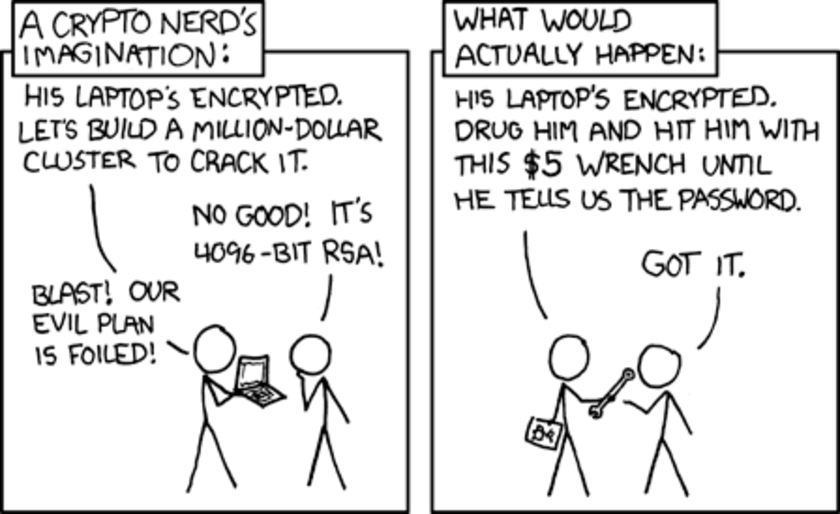
\includegraphics[width=100mm]{pic/rubberhose} 
\end{center}
\end{figure}
\end{frame}
\begin{frame}\frametitle{Outline}
\begin{itemize}
\item Classic cryptography, Perfect Secrets
\item Private Key Encryption, MAC, Block Cipher, OWF
\item Number Theory, Factoring and Discrete Log
\item Key Management, Public Key, Digital Signature
\item TPD, Random Oracle Model
\item Cryptographic Protocols (Many magics here)
\end{itemize}
\end{frame}
\begin{frame}\frametitle{Syllabus [in Chinese]}
\begin{figure}
\begin{center}
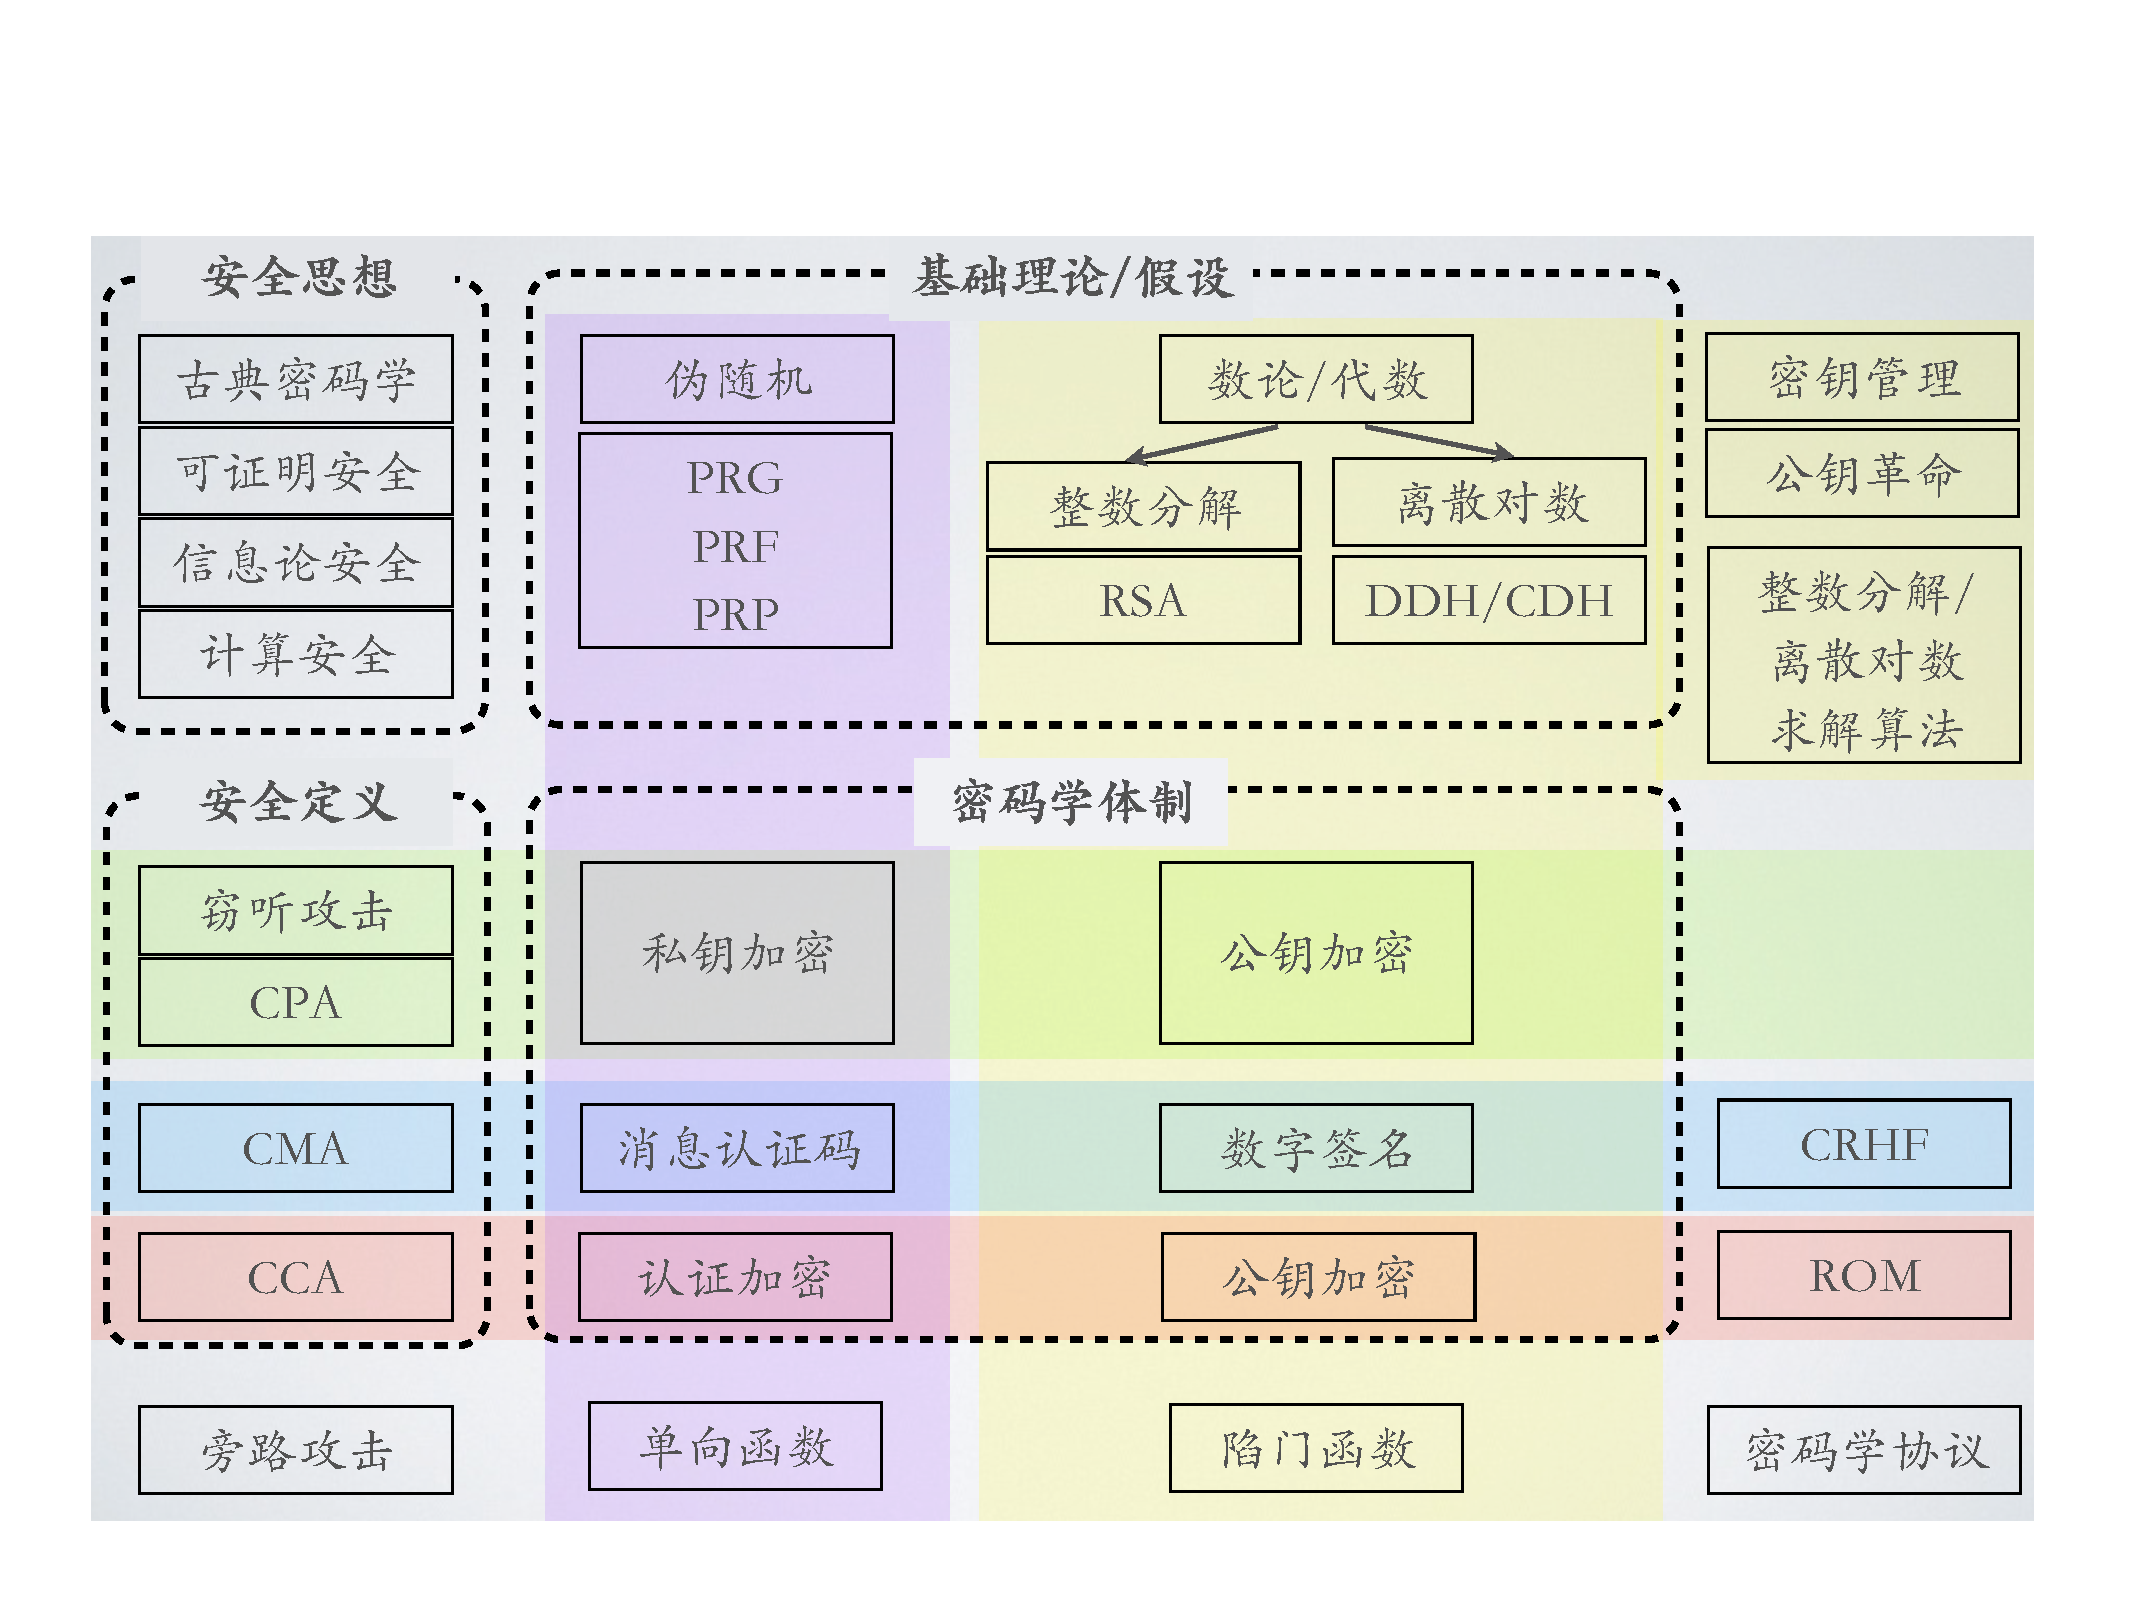
\includegraphics[width=100mm]{pic/syllabus} 
\end{center}
\end{figure}
\end{frame}
\begin{frame}\frametitle{We will learn from Turing Award recipients}
\begin{itemize}
\item{1995} M. Blum
\item{2000} A. Yao
\item{2002} R. Rivest, A. Shamir, L. Adleman
\item{2012} S. Micali, S. Goldwasser
\item{2013} L. Lamport
\item{2015} M. E. Hellman, W. Diffie
\end{itemize}	
\end{frame}


\begin{frame}\frametitle{Securing Key vs Obscuring Algorithm}
\begin{itemize}
\item Easier to maintain secrecy of a short key
\item In case the key is exposed, easier for the honest parties to change the key
\item In case many pairs of people, easier to use the same algorithm, but different keys
\end{itemize}
\begin{alertblock}{Kerckhoffs's principle}
\begin{quote}
The cipher method must not be required to be secret, and it must be able to fall into the hands of the enemy without inconvenience.
\end{quote}	
\end{alertblock}
\end{frame}

\begin{frame}\frametitle{The Syntax of Encryption}
\begin{figure}
\begin{center}
\begin{tikzpicture}
\node (sender) [minimum size=1cm] {}; \Alice{0}{0}{0.4};
\node (bart) [below of = sender, node distance = 0.7cm] {Alice};
\node (enc) [draw, right of = sender, rounded corners=1ex,node distance = 2cm] {$\mathsf{Enc}$};
\node (k1) [above of = enc, node distance = 1cm] {$k$};
\node (c) [right of = enc, node distance = 2cm] {$c$};
\node (gen) [draw, above of = c, rounded corners=1ex,node distance = 1cm] {$\mathsf{Gen}$};
\node (adv) [below of = c, node distance = 1cm, minimum size=1cm] {}; \Evil{4cm}{-1cm}{0.4};
\node (burns) [below of = adv, node distance = 0.7cm] {Adversary};
\node (dec) [draw, right of = c, rounded corners=1ex,node distance = 2cm] {$\mathsf{Dec}$};
\node (k2) [above of = dec, node distance = 1cm] {$k$};
\node (receiver) [right of = dec, node distance = 2cm, minimum size=1cm] {}; \Bob{8cm}{0}{0.4};
\node (lisa) [below of = receiver, node distance = 0.7cm] {Bob};
\draw[-latex] (sender) -- (enc) node [midway, above] {$m$};
\draw (enc) -- (c); \draw[-latex] (c) -- (dec);
\draw[-latex] (dec) -- (receiver) node [midway, above] {$m$};
\draw[-latex] (k1) -- (enc);
\draw[-latex] (gen) -- (k1);
\draw[-latex] (gen) -- (k2);								
\draw[-latex] (k2) -- (dec);		
\end{tikzpicture}
\end{center}
\end{figure}
\begin{itemize}
\item key $k \in \mathcal{K}$, plaintext (or message) $m \in \mathcal{M}$, ciphertext $c \in \mathcal{C}$
\item \textbf{Key-generation} algorithm~$k \gets \mathsf{Gen}$
\item \textbf{Encryption} algorithm~$c:= \mathsf{Enc}_k(m)$
\item \textbf{Decryption} algorithm~$m:= \mathsf{Dec}_k(c)$
\item \textbf{Encryption scheme}: $\Pi = (\mathsf{Gen}, \mathsf{Enc}, \mathsf{Dec})$
\item \textbf{Basic correctness requirement}: $\mathsf{Dec}_k(\mathsf{Enc}_k(m)) = m$
\end{itemize}
\end{frame}

\begin{frame}\frametitle{One-Time Pad (Vernam's Cipher)}

\begin{itemize}
	\item $\mathcal{M} = \mathcal{K} = \mathcal{C} = \{0,1\}^{\ell}$.
	\item $\mathsf{Gen}$ chooses a $k$ randomly with probability exactly $2^{-\ell}$.
	\item $c := \mathsf{Enc}_k(m) = k \oplus m$. 
	\item $m := \mathsf{Dec}_k(c) = k \oplus c$. 
\end{itemize}
\begin{theorem}
The one-time pad encryption scheme is perfectly-secret.
\end{theorem}
\end{frame}

\begin{frame}\frametitle{Definition of `Perfect Secrecy'}
\textbf{Intuition}: An adversary knows the probability distribution over $\mathcal{M}$. $c$ should have no effect on the knowledge of the adversary; the a \emph{posteriori} likelihood that some $m$ was sent should be no different from the a \emph{priori} probability that $m$ would be sent. 
\begin{definition}
$\Pi$ over $\mathcal{M}$ is \textbf{perfectly secret} if for every probability distribution over $\mathcal{M}$, $\forall m \in \mathcal{M}$ and $\forall c \in \mathcal{C}$ for which $\Pr[C = c] > 0$:
\[ \Pr[M=m | C=c] = \Pr[M=m].\]
\end{definition}
\textbf{Simplify}: non-zero probabilities for $\forall m \in \mathcal{M}$ and $\forall c \in \mathcal{C}$.\\

\begin{exampleblock}{Is the below scheme perfectly secret?}{ For $\mathcal{M}=\mathcal{K} = \{ 0,1 \} , \mathsf{Enc}_k(m)= m \oplus k$.}\end{exampleblock}
\end{frame}

\begin{frame}\frametitle{Two Time Pad: Real World Cases}
Only used once for the same key, otherwise
\[c\oplus c'=(m\oplus k)\oplus (m'\oplus k)=m\oplus m'.\]
Learn $m$ from $m\oplus m'$ due to the redundancy of language.
\begin{exampleblock}{MS-PPTP (Win NT)}
\begin{figure}
\begin{center}
\begin{tikzpicture}
\node (sender) [minimum size=1cm,label=below:Client, label=above:$k$] {}; \Alice{0}{0}{0.4};
\node (c) at ($(sender)+(4cm,0.5cm)$) {$\left[ m_1\|m_2\|m_3\right] \oplus PRG(k)$};
\node (c1) [below of = c, node distance = 1cm] {$\left[s_1\|s_2\|s_3\right] \oplus PRG(k)$};
\node (receiver) at ($(sender)+(8cm,0)$) [minimum size=1cm,label=below:Server, label=above:$k$] {}; \Bob{8cm}{0}{0.4};
\draw[-latex] (sender.east |- c) -- (c) -- (receiver.west |- c);
\draw[-latex] (receiver.west |- c1) -- (c1) -- (sender.east |- c1);
\end{tikzpicture}
\end{center}
\end{figure}
Improvement: use two keys for C-to-S and S-to-C separately.
\end{exampleblock}
\end{frame}
\begin{frame}\frametitle{Eavesdropping Indistinguishability Experiment}
The eavesdropping indistinguishability experiment $\mathsf{PrivK}^{\mathsf{eav}}_{\mathcal{A},\Pi}(n)$:
\begin{enumerate}
	\item $\mathcal{A}$ is given input $1^n$, outputs $m_0, m_1$ of the same length
	\item $k \gets \mathsf{Gen}(1^n)$, a random bit $b \gets \{0,1\}$ is chosen. Then $c \gets \mathsf{Enc}_k(m_b)$ (challenge ciphertext) is given to $\mathcal{A}$
	\item $\mathcal{A}$ outputs $b'$. If $b' = b$, $\mathsf{PrivK}^{\mathsf{eav}}_{\mathcal{A},\Pi}=1$, otherwise 0
\end{enumerate}
\begin{figure}
\begin{center}
\begin{tikzpicture}
%\node (A) at (0,0) {\Homer};
%\node (B) [right of = A, node distance = 4cm] {\Left\Burns};
\node (A) at (0,0) [minimum size=1cm] {}; \Charlie{0}{0}{0.4};
\node (B) [right of = A, node distance = 4cm, minimum size=1cm] {}; \Evil{4cm}{0}{0.4};
\node (1a) [below of=A, node distance=1cm] {};
\node (1b) [below of=B, node distance=1cm] {$m_0, m_1$};
\draw[-latex] (1b) -- (1a) node [midway,above] {};
\node (2a) [below of=1a, node distance=0.5cm] {Gen $b, k$};
\node (2b) [below of=1b, node distance=0.5cm] {};
%\draw[-latex] (2b) -- (2a) node [midway,above] {};
%\node (3a) [below of=2a, node distance=0.5cm] {};
%\node (3b) [below of=2b, node distance=0.5cm] {};
\node (4a) [below of=2a, node distance=0.5cm] {$\mathsf{Enc}_k(m_b)$};
\node (4b) [below of=2b, node distance=0.5cm] {};
\draw[-latex] (4a) -- (4b) node [midway,above] {};
\node (5a) [below of=4a, node distance=0.5cm] {};
\node (5b) [below of=4b, node distance=0.5cm] {$b'$};
\draw[-latex] (5b) -- (5a) node [midway,above] {};
\node (6a) [below of=5a, node distance=0.5cm] {};
\node (6b) [below of=5b, node distance=0.5cm] {};
\node (result) [right of = 6a, node distance = 2cm] {Win if $b = b'$};
\end{tikzpicture}

\end{center}
\end{figure}
\end{frame}
\begin{frame}\frametitle{Defining Private-key Encryption Security}
\begin{definition}\label{def:ind}
$\Pi$ has \textbf{indistinguishable encryptions in the presence of an eavesdropper} if $\forall$ \textsc{ppt} $\mathcal{A}$, $\exists$ a negligible function $\mathsf{negl}$ such that
\[ \Pr\left[\mathsf{PrivK}^{\mathsf{eav}}_{\mathcal{A},\Pi}(n)=1\right] \le \frac{1}{2} + \mathsf{negl}(n),
\]
where the probability it taken over the random coins used by $\mathcal{A}$.
\end{definition}
\end{frame}

\begin{frame}\frametitle{Conceptual Points of Pseudorandomness}
\begin{itemize}
\item True randomness can not be generated by a describable mechanism
\item Pseudorandom looks truly random for the observers who don't know the mechanism 
\item No fixed string can be ``pseudorandom'' which refers to a distribution
\item \alert{Q: is it possible to definitively prove randomness?}
\end{itemize}
\begin{figure}
\begin{center}
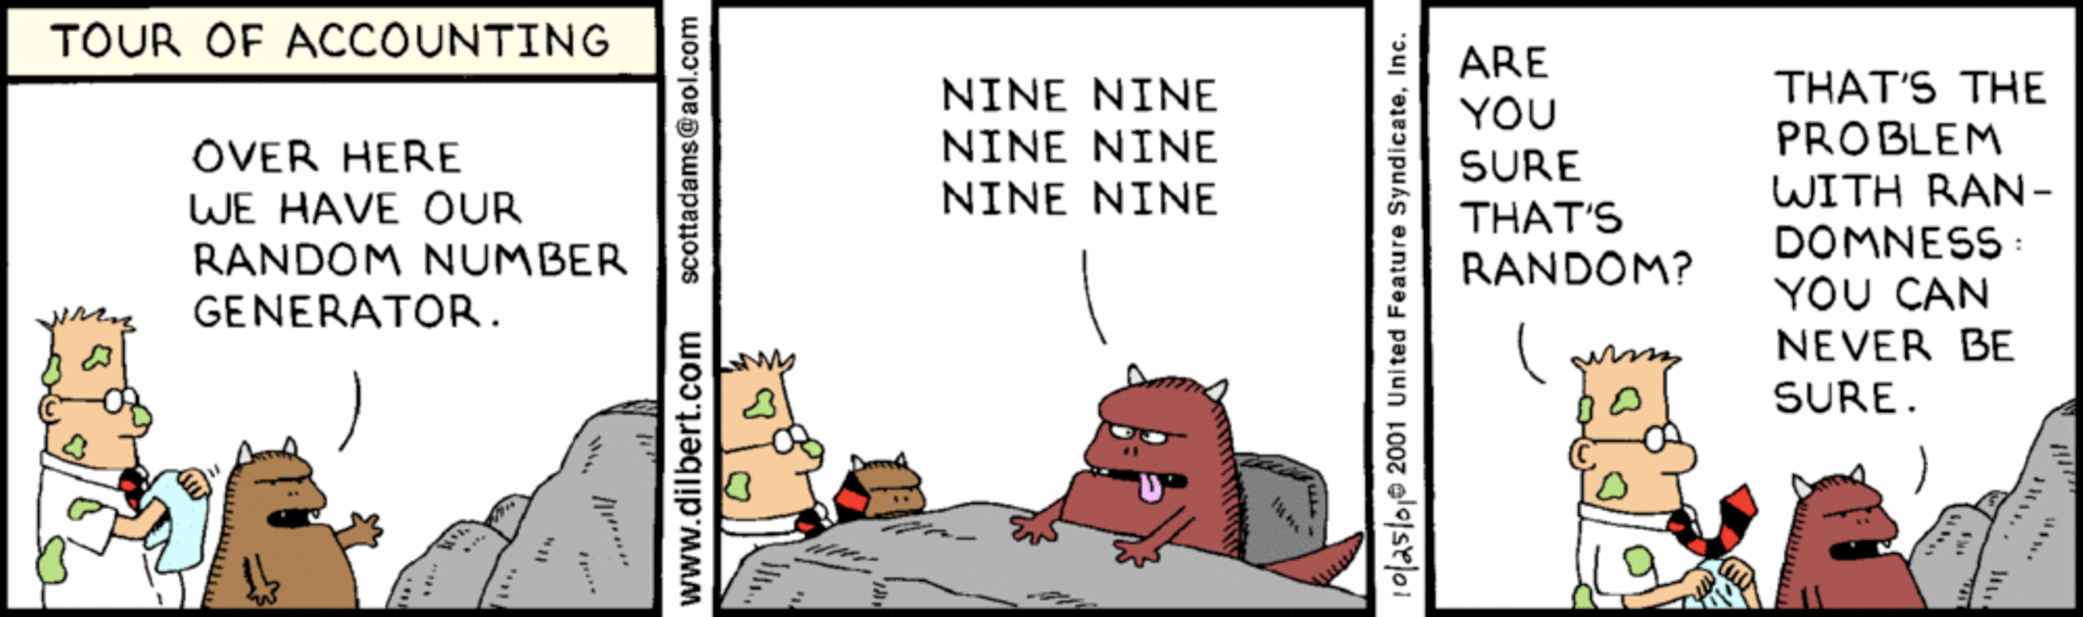
\includegraphics[width=100mm]{pic/random-color} 
\end{center}
\end{figure}
\end{frame}


\begin{frame}\frametitle{Intuition for Defining Pseudorandom}
\textbf{Intuition}: Generate a long string from a short truly random seed, and the pseudorandom string is indistinguishable from truly random strings.
\begin{figure}
\begin{center}
\begin{tikzpicture}
%\node (A) at (0,0) {\Homer};
%\node (B) [right of = A, node distance = 4cm] {\Left\Burns};
\node (A) at (0,0) [minimum size=1cm] {}; \Charlie{0}{0}{0.4};
\node (B) [right of = A, node distance = 4cm, minimum size=1cm] {}; \Evil{4cm}{0}{0.4};
\node (1a) [below of=A, node distance=1cm] {choose a truly random};
\node (1b) [below of=B, node distance=1cm] {Distinguisher $D$};
%\draw[-latex] (1b) -- (1a) node [midway,above] {};
\node (2a) [below of=1a, node distance=0.5cm] {string or generate a};
\node (2b) [below of=1b, node distance=0.5cm] {};
%\draw[-latex] (2b) -- (2a) node [midway,above] {};
\node (3a) [below of=2a, node distance=0.5cm] {pseudorandom one};
\node (3b) [below of=2b, node distance=0.5cm] {};
\node[draw, fit=(1a) (2a) (3a), rounded corners=1ex] {};
\node (4a) [below of=3a, node distance=1cm] {the string};
\node (4b) [below of=3b, node distance=1cm] {};
\draw[-latex] (4a) -- (4b) node [midway,above] {};
\node (5a) [below of=4a, node distance=0.5cm] {};
\node (5b) [below of=4b, node distance=0.5cm] {1 or 0};
\draw[-latex] (5b) -- (5a) node [midway,above] {};
%\node (6a) [below of=5a, node distance=0.5cm] {};
%\node (6b) [below of=5b, node distance=0.5cm] {};
%\node (result) [right of = 6a, node distance = 2cm] {};
\end{tikzpicture}

\end{center}
\end{figure}
\end{frame}
\begin{frame}\frametitle{Definition of Pseudorandom Generators}
\begin{definition}\label{def:pg}
A deterministic polynomial-time algorithm $G : \{0,1\}^n \to \{0,1\}^{\ell(n)}$ is a \textbf{pseudorandom generator (PRG)} if
\begin{enumerate}
\item (Expansion:) $\forall n, \ell(n) > n$.
\item (Pseudorandomness): $\forall\;$ \textsc{ppt} distinguishers $D$,
\[ \left|\Pr[D(r)=1] - \Pr[D(G(s))=1]\right| \le \mathsf{negl}(n),
\]
where $r$ is chosen \emph{u.a.r} from $\{0,1\}^{\ell(n)}$, the \textbf{seed} $s$ is chosen \emph{u.a.r} from $\{0,1\}^n$. $\ell(\cdot)$ is the \textbf{expansion factor} of $G$.
\end{enumerate}
\end{definition}
\begin{itemize}
\item Pseudorandomness means being \textbf{next-bit unpredictable},\\
$G$ passes all next bit tests $\iff$ $G$ passes all statistical tests.
\item \textbf{Existence}: Under the weak assumption that \emph{one-way functions} exists, or $\mathcal{P} \ne \mathcal{NP}$
\end{itemize}
\end{frame}
\begin{frame}\frametitle{A Secure Fixed-Length Encryption Scheme}
\begin{columns}[t]
\begin{column}{4cm}
\begin{figure}
\begin{center}
\begin{tikzpicture}
\node (k) {$k$};
\node (pg) [draw, below of = k, rounded corners=1ex,node distance = 1.5cm] {$G$};
\node (pad) [minimum width=2cm, draw, shape = rectangle, below of = pg, node distance = 1.5cm] {Pad};
\node (xor) [below of = pad, circle, node distance = 1.2cm, draw] {};
\draw[-] (xor.north) -- (xor.south);
\draw[-] (xor.east) -- (xor.west);
\node (pt) [left of = xor, node distance = 1.5cm] {$m$};
\node (ct) [right of = xor, node distance = 1.5cm] {$c$};
\draw[-latex] (k) -- (pg);
\draw[-latex] (pg) -- (pad);
\draw[-latex] (pad) -- (xor);
\draw[-latex] (pt) -- (xor);
\draw[-latex] (xor) -- (ct);
\end{tikzpicture}
\end{center}
\end{figure}
\end{column}
\begin{column}{6cm}
\begin{construction}\label{con:fl}
\begin{itemize}
\item $|G(k)| = \ell(|k|)$, $m \in \{0,1\}^{\ell(n)}$.
\item $\mathsf{Gen}$: $k \in \{0,1\}^n$.
\item $\mathsf{Enc}$: $c := G(k)\oplus m$.
\item $\mathsf{Dec}$: $m := G(k)\oplus c$.
\end{itemize}
\end{construction}
\begin{theorem}\label{the:flt}
This fixed-length encryption scheme has indistinguishable encryptions in the presence of an eavesdropper.
\end{theorem}
\end{column}
\end{columns}
\end{frame}
\begin{frame}\frametitle{Secure Multiple Encryptions Using a Stream Cipher}
\begin{figure}
\begin{center}
\begin{tikzpicture}
\node (sm) {};
\foreach \x in {1, 2, 3} {
\node (g\x) at ($(sm) + \x*(2.8cm,0) - (4cm,0)$)  [] {};
\node (pa\x) [right of = g\x, node distance = 1.8cm, minimum width = 2.8cm, draw] {Part \x};
\node (xor\x) [below of = pa\x, circle, node distance = 1cm, draw] {};
\draw[-] (xor\x.north) -- (xor\x.south);
\draw[-] (xor\x.east) -- (xor\x.west);
\node (pt\x) [left of = xor\x, node distance = 0.9cm] {$m_\x$};
\node (ct\x) [right of = xor\x, node distance = 0.8cm] {$c_\x$};
\draw[-latex] (pa\x) -- (xor\x);
\draw[-latex] (pt\x) -- (xor\x);
\draw[-latex] (xor\x) -- (ct\x);
}
\node (gg) at ($(sm) - (1.7cm,0)$)  [rounded corners=1ex,draw] {$G$};
\draw[-latex] (gg) -- (pa1);
\node (iv) [below=0.5cm of gg] {$K$};
\draw[-latex] (iv) -- (gg.south);
%\node (k) [left of = gg, node distance = 1cm] {$K$};
%\draw[-latex] (k) -- (gg);

\node (usm) [below of=sm, node distance=3.5cm] {};
\foreach \x in {1, 2, 3} {
\node (ug\x) at ($(usm) + \x*(3.3cm,0) - (5cm,0)$)  [rounded corners=1ex,draw] {$G$};
\node (uk\x) [above=0.5cm of ug\x] {};
\draw[-latex] (uk\x) -- (ug\x.north);
\node (uiv\x) [below=0.5cm of ug\x] {$IV_\x$};
\draw[-latex] (uiv\x) -- (ug\x.south);
\node (upa\x) [right of = ug\x, node distance = 1.8cm, minimum width = 2cm, draw] {Part \x};
\node (uxor\x) [below of = upa\x, circle, node distance = 1cm, draw] {};
\draw[-] (uxor\x.north) -- (uxor\x.south);
\draw[-] (uxor\x.east) -- (uxor\x.west);
\node (upt\x) [left of = uxor\x, node distance = 0.9cm] {$m_\x$};
\node (uct\x) [right of = uxor\x, node distance = 0.8cm] {$c_\x$};
\draw[-latex] (upa\x) -- (uxor\x);
\draw[-latex] (upt\x) -- (uxor\x);
\draw[-latex] (uxor\x) -- (uct\x);
\draw[-latex] (ug\x) -- (upa\x);
}
\draw[-] (uk1.south) node [left] {$K$} -- (uk3.south);
\node [above of= upt2, node distance=2.5cm] {\emph{Synchronized Mode}};
\node [below of= upt2] {\emph{Unsynchronized Mode}};
\end{tikzpicture}
\end{center}
\end{figure}
Initial vector $IV$ is chosen \emph{u.a.r} and public\\
\alert{Q: which mode is better in your opinion?}
\end{frame}
\begin{frame}\frametitle{Related Keys: Real World Cases}
Keys (the $IV$-key pair) for multiple enc. must be independent
\begin{exampleblock}{Attacks on 802.11b WEP}
Unsynchronized mode: $\mathsf{Enc}(m_i) := \left< IV_i, G(IV_i\|k) \oplus m_i\right>$\\
\begin{itemize}
\item Length of $IV$ is 24 bits, repeat $IV$ after $2^{24} \approx$ 16M frames
\item On some WiFi cards, $IV$ resets to $0$ after power cycle
\item $IV_i = IV_{i-1} + 1$. For RC4, recover $k$ after 40,000 frames
\end{itemize}
\end{exampleblock}
\end{frame}
\begin{frame}\frametitle{Chosen-Plaintext Attacks (CPA)}
\textbf{CPA}: the adversary has the ability to obtain the encryption of plaintexts of its choice
\begin{exampleblock}{A story in WWII}
\begin{itemize}
\item Navy cryptanalysts believe the ciphertext ``AF'' means ``Midway island'' in Japanese messages
\item But the general did not believe that Midway island would be attacked
\item Navy cryptanalysts sent a plaintext that the freshwater supplies at Midway island were low
\item Japanese intercepted the plaintext and sent a ciphertext that ``AF'' was low in water
\item The US forces dispatched three aircraft carriers and won
\end{itemize}
\end{exampleblock}
\end{frame}
\begin{frame}\frametitle{Security Against CPA}
The CPA indistinguishability experiment $\mathsf{PrivK}^{\mathsf{cpa}}_{\mathcal{A},\Pi}(n)$:
\begin{enumerate}
	\item $k \gets \mathsf{Gen}(1^n)$
	\item $\mathcal{A}$ is given input $1^n$ and \textbf{oracle access} $\mathcal{A}^{\mathsf{Enc}_k(\cdot)}$ to $\mathsf{Enc}_k(\cdot)$, outputs $m_0, m_1$ of the same length
	\item $b \gets \{0,1\}$. Then $c \gets \mathsf{Enc}_k(m_b)$ is given to $\mathcal{A}$
	\item $\mathcal{A}$ \textbf{continues to have oracle access} to $\mathsf{Enc}_k(\cdot)$, outputs $b'$
	\item If $b' = b$, $\mathcal{A}$ succeeded $\mathsf{PrivK}^{\mathsf{cpa}}_{\mathcal{A},\Pi}=1$, otherwise 0
\end{enumerate}
\begin{figure}
\begin{center}
\begin{tikzpicture}
%\node (A) at (0,0) {\Homer};
%\node (B) [right of = A, node distance = 4cm] {\Left\Burns};
\node (A) at (0,0) [minimum size=1cm] {}; \Charlie{0}{0}{0.4};
\node (B) [right of = A, node distance = 4cm, minimum size=1cm] {}; \Evil{4cm}{0}{0.4};
\node (enc) [draw, rounded corners=1ex, right of=B, node distance = 2cm] {$\mathsf{Enc}_k(\cdot)$};
\draw[-latex] (B) to [bend left=15,-latex,above] (enc);
\draw[-latex] (enc) to [bend left=15,-latex,below] (B);
\node (k) [left of=A, node distance = 1.5cm] {Gen $k$};
\node (1a) [below of=A, node distance=1cm] {};
\node (1b) [below of=B, node distance=1cm] {$m_0, m_1$};
\draw[-latex] (1b) -- (1a) node [midway,above] {};
\node (2a) [below of=1a, node distance=0.5cm] {Gen $b$};
\node (2b) [below of=1b, node distance=0.5cm] {};
%\draw[-latex] (2b) -- (2a) node [midway,above] {};
%\node (3a) [below of=2a, node distance=0.5cm] {};
%\node (3b) [below of=2b, node distance=0.5cm] {};
\node (4a) [below of=2a, node distance=0.5cm] {$\mathsf{Enc}_k(m_b)$};
\node (4b) [below of=2b, node distance=0.5cm] {};
\draw[-latex] (4a) -- (4b) node [midway,above] {};
\node (5a) [below of=4a, node distance=0.5cm] {};
\node (5b) [below of=4b, node distance=0.5cm] {$b'$};
\draw[-latex] (5b) -- (5a) node [midway,above] {};
\node (6a) [below of=5a, node distance=0.5cm] {};
\node (6b) [below of=5b, node distance=0.5cm] {};
\node (result) [right of = 6a, node distance = 2cm] {Win if $b = b'$};
\end{tikzpicture}

\end{center}
\end{figure}
\end{frame}
\begin{frame}\frametitle{Concepts on Pseudorandom Functions}
\begin{figure}
\begin{center}
\begin{tikzpicture}[uk/.style={inner sep=1pt, minimum width=10pt, circle, fill=red!50},kk/.style={inner sep=1pt, minimum width=10pt, fill=blue!50, circle}]
\node (K) at (2.2cm,0) [ellipse,minimum width=1cm,minimum height=2cm,draw] {}; 
\node (k) [above of=K,node distance=1.2cm] {$K$}; 
\foreach \i in {1, 2, 3} {
\node (X\i) at (\i*3.3cm,0) [ellipse,minimum width=1cm,minimum height=2cm,draw] {}; 
\node (x) [above of=X\i,node distance=1.2cm] {$X$}; 
\node (Y\i) [right of=X\i,ellipse,minimum width=1cm,minimum height=2cm,node distance=1.5cm,draw] {};
\node (y) [above of=Y\i,node distance=1.2cm] {$Y$}; 
}
\node (cr) at ($(X1)+(0cm,-1.5cm)$) [] {\footnotesize $F: K \times X \to Y$};
\node (cr) at ($(X1)+(0cm,-2cm)$) [] {\footnotesize 2D function};
\node (k1) at ($(K)+(0,0.3cm)$) [kk] {\tiny };
\node (k2) at ($(K)+(0,-0.3cm)$) [uk] {\tiny };
\node (x1) at ($(X1)+(0,0.3cm)$) [kk] {\tiny };
\node (x2) at ($(X1)+(0,-0.3cm)$) [kk] {\tiny };
\node (y1) at ($(Y1)+(0,0.3cm)$) [kk] {\tiny };
\node (y2) at ($(Y1)+(0,-0.3cm)$) [kk] {\tiny };
\draw[-latex,red!50] (x1) -- (y1);
\draw[-latex,red!50] (x2) -- (y2);
\draw[-latex] (x1) -- (y2);
\draw[-latex] (x2) -- (y1);
\draw[-] (k1) -- (x1);
\draw[-] (k1) -- (x2);
\draw[-,red!50] (k2) -- (x1);
\draw[-,red!50] (k2) -- (x2);
\node (2pr) at ($(X2)+(0.75cm,-1.5cm)$) [] {\footnotesize $F_k(x) \overset{\text{def}}{=} F(k,x)$};
\node (2pr) at ($(X2)+(0.75cm,-2cm)$) [] {\footnotesize Keyed function};
\node (x1) at ($(X2)+(0,0.3cm)$) [kk] {\tiny };
\node (x2) at ($(X2)+(0,-0.3cm)$) [kk] {\tiny };
\node (y1) at ($(Y2)+(0,0.3cm)$) [kk] {\tiny };
\node (y2) at ($(Y2)+(0,-0.3cm)$) [kk] {\tiny };
\draw[-latex] (x1) -- (y2);
\draw[-latex] (x2) -- (y1);
\node (pr) at ($(X3)+(0.75cm,-1.5cm)$) [] {\footnotesize $f : X \to Y$};
\node (pr) at ($(X3)+(0.75cm,-2cm)$) [] {\footnotesize Look-up table};
\node (x1) at ($(X3)+(0,0.3cm)$) [kk] {\tiny };
\node (x2) at ($(X3)+(0,-0.3cm)$) [kk] {\tiny };
\node (y1) at ($(Y3)+(0,0.3cm)$) [kk] {\tiny };
\node (y2) at ($(Y3)+(0,-0.3cm)$) [kk] {\tiny };
\draw[-latex] (x1) -- (y1);
\draw[-latex] (x2) -- (y1);
\end{tikzpicture}

\end{center}
\end{figure}
\begin{itemize}
\item \textbf{Keyed function} $F : \{0,1\}^* \times \{0,1\}^* \to \{0,1\}^*$ \\
$F_k : \{0,1\}^* \to \{0,1\}^*$, $F_k(x) \overset{\text{def}}{=} F(k,x)$
\item \textbf{Look-up table $f$}: $\{0,1\}^n \to \{0,1\}^n$ with size \alert{ = ? bits} %$n\cdot2^n$.
\item \textbf{Function family $\mathsf{Func}_n$}: all functions $\{0,1\}^n \to \{0,1\}^n$. $|\mathsf{Func}_n| = 2^{n\cdot2^n}$
\item \textbf{Length Preserving}: $\ell_{key}(n) = \ell_{in}(n) = \ell_{out}(n)$
\end{itemize}
\end{frame}
\begin{frame}\frametitle{CPA-Security from Pseudorandom Function}
\begin{columns}[t]
\begin{column}{4cm}
\begin{figure}
\begin{center}
\begin{tikzpicture}
\node (r) {$r$};
\node (pg) [draw, below of = r, rounded corners=1ex,node distance = 1.5cm] {$F$};
\node (k) [left of = pg, node distance = 1.5cm] {$k$};
\node (pad) [minimum width=2cm, draw, shape = rectangle, below of = pg, node distance = 1.5cm] {Pad};
\node (xor) [below of = pad, circle, node distance = 1.2cm, draw] {};
\draw[-] (xor.north) -- (xor.south);
\draw[-] (xor.east) -- (xor.west);
\node (pt) [left of = xor, node distance = 1.5cm] {$m$};
\node (ct) [right of = xor, node distance = 1.5cm] {$c$};
\draw[-latex] (r) -- (pg);
\draw[-latex] (pg) -- (pad);
\draw[-latex] (pad) -- (xor);
\draw[-latex] (pt) -- (xor);
\draw[-latex] (xor) -- (ct);
\draw[-latex] (r) -| (ct);
\draw[-latex] (k) -- (pg);
\end{tikzpicture}
\end{center}
\end{figure}
\end{column}
\begin{column}{6cm}
\begin{construction}\label{thm:cpa}
\begin{itemize}
\item Fresh random string $r$.
\item $F_k(r)$: $\abs{k} = \abs{m} = \abs{r} = n$.
\item $\mathsf{Gen}$: $k \in \{0,1\}^n$.
\item $\mathsf{Enc}$: $s := F_k(r)\oplus m$, $c := \left<r, s\right>$.
\item $\mathsf{Dec}$: $m := F_k(r)\oplus s$.
\end{itemize}
\end{construction}
\begin{theorem}\label{thm:prf}
If $F$ is a PRF, this fixed-length encryption scheme $\Pi$ is CPA-secure.
\end{theorem}
\end{column}
\end{columns}
\end{frame}
\begin{frame}\frametitle{Pseudorandom Permutations}
\begin{itemize}
\item \textbf{Bijection}: $F$ is one-to-one and onto
\item \textbf{Permutation}: A bijective function from a set to itself
\item \textbf{Keyed permutation}: $\forall k, F_k(\cdot)$ is permutation
\item $F$ is a bijection $\iff F^{-1}$ is a bijection
\end{itemize}
\begin{definition}
An efficient, keyed permutation $F$ is a \textbf{strong pseudorandom permutation (PRP)} if
$\forall\;$ \textsc{ppt} distinguishers $D$,
\[ \left|\Pr[D^{F_k(\cdot),F_k^{-1}(\cdot)}(1^n)=1] - \Pr[D^{f(\cdot),f^{-1}(\cdot)}(1^n)=1]\right| \le \mathsf{negl}(n),
\]
where $f$ is chosen \emph{u.a.r} from the set of permutations on $n$-bit strings.
\end{definition}
\begin{alertblock}{If $F$ is a pseudorandom permutation then is it a PRF?}
\end{alertblock}
\end{frame}
\begin{frame}\frametitle{Electronic Code Book (ECB) Mode}
\begin{figure}
\begin{center}
\begin{tikzpicture}
\foreach \x in {1, 2, 3} {
\node (f\x) at ($\x*(2.5cm,0)$) [minimum size=1.25cm,rounded corners=1ex,draw] {\Large $F_k$};
\node (m\x) [above of=f\x, node distance=2cm] {$m_\x$};
\node (c\x) [below of=f\x, node distance=2cm] {$c_\x$};
\draw[-latex] (m\x) -- (f\x);
\draw[-latex] (f\x) -- (c\x);
}
\end{tikzpicture}

\end{center}
\end{figure}
\begin{itemize}
\item \alert{Q: is it indistinguishable in the presence of an eavesdropper?}
\item \alert{Q: can $F$ be any PRF?}
\end{itemize}
\end{frame}
\begin{frame}\frametitle{Attack on ECB mode}
\begin{figure}
\begin{center}
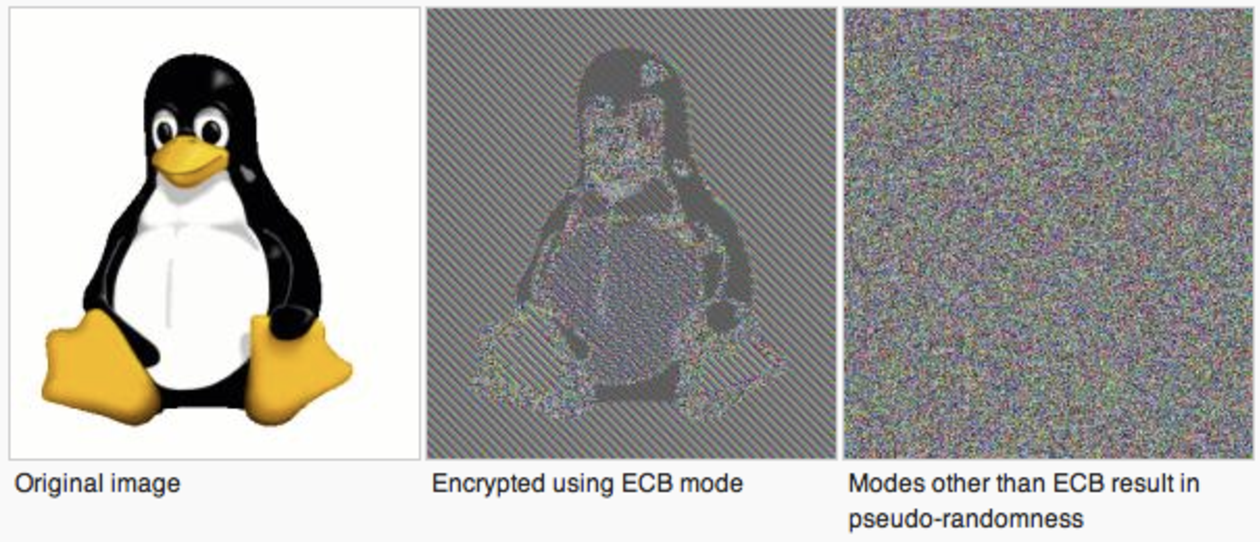
\includegraphics[width=100mm]{pic/ecb} 
\end{center}
\end{figure}
\end{frame}
\begin{frame}\frametitle{Cipher Block Chaining (CBC) Mode}
\begin{figure}
\begin{center}
\begin{tikzpicture}
\foreach \x in {1, 2, 3} {
\node (f\x) at ($\x*(2.5cm,0)$) [minimum size=1.25cm,rounded corners=1ex,draw] {\Large $F_k$};
\node (m\x) [above of=f\x, node distance=2.5cm] {$m_\x$};
\node (c\x) [below of=f\x, node distance=1.5cm] {$c_\x$};
\node (p\x) [above of=f\x, node distance=1.5cm, circle, draw] {};
\draw[-] (p\x.north) -- (p\x.south);
\draw[-] (p\x.east) -- (p\x.west);
\draw[-latex] (m\x) -- (p\x);
\draw[-latex] (p\x) -- (f\x);
\draw[-latex] (f\x) -- (c\x);
}

\node (iv) [left of=p1, node distance=1.5cm] {$IV$};
\node (iv2) [left of=c1, node distance=1.5cm] {$IV$};
\draw[-latex] (iv) -- (iv2);
\draw[-latex] (iv) -- (p1);

\foreach \x in {1, 2} {
\draw[-latex] ($(c\x) + (0,0.6cm)$) -| +(1.25cm,2.4cm) -- ($(p\x.west) + (2.5cm,0)$);
}

\end{tikzpicture}
\end{center}
\end{figure}
\begin{itemize}
\item $IV$: initial vector, a fresh random string.
\end{itemize}
\end{frame}
\begin{frame}\frametitle{Output Feedback (OFB) Mode}
\begin{figure}
\begin{center}
\begin{tikzpicture}
\foreach \x in {1, 2, 3} {
\node (f\x) at ($\x*(2.5cm,0)$) [minimum size=1.25cm,rounded corners=1ex,draw] {\Large $F_k$};
\node (c\x) [below of=f\x, node distance=2.5cm] {$c_\x$};
\node (p\x) [below of=f\x, node distance=1.5cm, circle, draw] {};
\node (m\x) [left of=p\x, node distance=1.0cm] {$m_\x$};
\draw[-] (p\x.north) -- (p\x.south);
\draw[-] (p\x.east) -- (p\x.west);
\draw[-latex] (m\x) -- (p\x);
\draw[-latex] (f\x) -- (p\x);
\draw[-latex] (p\x) -- (c\x);
}

\node (iv2) [left of=c1, node distance=1.5cm] {$IV$};
\node (iv) [above of=iv2, node distance=4cm] {$IV$};
\draw[-latex] (iv) -- (iv2);
\draw[-latex] (iv) -| (f1.north);

\foreach \x in {1, 2} {
%\draw[-] ($(p\x) + (0,0.6cm)$) -| +(1.25cm,2.4cm);
%\draw[-latex] ($(p\x) + (1.25,3cm)$) -| ($(f\x.north) + (2.5cm,0)$);
\draw[-latex] ($(p\x) + (0,0.6cm)$) -| +(1.25cm,2.4cm) -| ($(f\x.north) + (2.5cm,0)$);
}

\end{tikzpicture}
\end{center}
\end{figure}
\end{frame}
\begin{frame}\frametitle{Counter (CTR) Mode}
\begin{figure}
\begin{center}
\begin{tikzpicture}
\foreach \x in {1, 2, 3} {
\node (f\x) at ($\x*(2.5cm,0)$) [minimum size=1.25cm,rounded corners=1ex,draw] {\Large $F_k$};
\node (c\x) [below of=f\x, node distance=2.5cm] {$c_\x$};
\node (p\x) [below of=f\x, node distance=1.5cm, circle, draw] {};
\node (m\x) [left of=p\x, node distance=1.0cm] {$m_\x$};
\node (ctr\x) [above of=f\x, node distance=1.5cm] {$\mathsf{ctr}+\x$};
\draw[-] (p\x.north) -- (p\x.south);
\draw[-] (p\x.east) -- (p\x.west);
\draw[-latex] (m\x) -- (p\x);
\draw[-latex] (f\x) -- (p\x);
\draw[-latex] (p\x) -- (c\x);
\draw[-latex] (ctr\x) -- (f\x);
}
\node (iv2) [left of=c1, node distance=1.5cm] {$\mathsf{ctr}$};
\node (iv) [above of=iv2, node distance=4cm] {$\mathsf{ctr}$};
\draw[-latex] (iv) -- (iv2);
\end{tikzpicture}
\end{center}
\end{figure}
\end{frame}

\begin{frame}[fragile]\frametitle{$IV$ Should Not Be Predictable}
If $IV$ is predictable, then CBC/OFB/CTR mode is not CPA-secure.\\
\begin{exampleblock}{Bug in SSL/TLS 1.0}
$IV$ for record $\#i$ is last CT block of record $\#(i-1)$.
\end{exampleblock}
\begin{exampleblock}{API in OpenSSL}
\verb#void AES_cbc_encrypt (# \\
\verb#    const unsigned char *in,# \\
\verb#    unsigned char       *out,# \\
\verb#    size_t              length,# \\
\verb#    const AES_KEY       *key,# \\
\verb#    unsigned char       *ivec,   #  \alert{\textbf{User supplies $IV$}} \\
\verb#    AES_ENCRYPT or AES_DECRYPT);# \\
\end{exampleblock}
\end{frame}
\begin{frame}\frametitle{Security Against CCA}
The CCA indistinguishability experiment $\mathsf{PrivK}^{\mathsf{cca}}_{\mathcal{A},\Pi}(n)$:
\begin{enumerate}
	\item $k \gets \mathsf{Gen}(1^n)$.
	\item $\mathcal{A}$ is given input $1^n$ and oracle access $\mathcal{A}^{\mathsf{Enc}_k(\cdot)}$ and $\mathcal{A}^{\mathsf{Dec}_k(\cdot)}$, outputs $m_0, m_1$ of the same length.
	\item $b \gets \{0,1\}$. $c \gets \mathsf{Enc}_k(m_b)$ is given to $\mathcal{A}$.
	\item $\mathcal{A}$ continues to have oracle access \alert{\textbf{except for $c$}}, outputs $b'$.
	\item If $b' = b$, $\mathcal{A}$ succeeded $\mathsf{PrivK}^{\mathsf{cca}}_{\mathcal{A},\Pi}=1$, otherwise 0.
\end{enumerate}
\begin{itemize}
\item In real world, the adversary might conduct CCA by influencing what gets decrypted
\begin{itemize}
\item If the communication is not authenticated, then an adversary may send certain ciphertexts on behalf of the honest party
\end{itemize}
\item CCA-security implies ``\textbf{non-malleability}''
\item None of the above scheme is CCA-secure
\end{itemize}
\end{frame}
\begin{frame}\frametitle{Padding-Oracle Attacks} 
\begin{itemize}
\item In a one-block CBC, by modifying the 1st byte of $IV$, attacker can learn whether $m$ is NULL. If yes, error will occur. 
\end{itemize}
\begin{columns}[c]
\column{.5\textwidth}
\begin{figure}
\begin{center}
\begin{tikzpicture}[scale=0.7, every node/.style={scale=0.7}]
\foreach \x in {1, 2, 3} {
\node (f\x) at ($\x*(2.5cm,0)$) [minimum size=1.25cm,rounded corners=1ex,draw] {\Large $F_k$};
\node (m\x) [above of=f\x, node distance=2.5cm] {$m_\x$};
\node (c\x) [below of=f\x, node distance=1.5cm] {$c_\x$};
\node (p\x) [above of=f\x, node distance=1.5cm, circle, draw] {};
\draw[-] (p\x.north) -- (p\x.south);
\draw[-] (p\x.east) -- (p\x.west);
\draw[-latex] (m\x) -- (p\x);
\draw[-latex] (p\x) -- (f\x);
\draw[-latex] (f\x) -- (c\x);
}

\node (iv) [left of=p1, node distance=1.5cm] {$IV$};
\node (iv2) [left of=c1, node distance=1.5cm] {$IV$};
\draw[-latex] (iv) -- (iv2);
\draw[-latex] (iv) -- (p1);

\foreach \x in {1, 2} {
\draw[-latex] ($(c\x) + (0,0.6cm)$) -| +(1.25cm,2.4cm) -- ($(p\x.west) + (2.5cm,0)$);
}

\end{tikzpicture}
\end{center}
\end{figure}
\column{.5\textwidth}
\begin{itemize}
\item append $\{b\}^b$ as a dummy block if $m$ is NULL
\item change the 1st byte of $IV$ from $x$ to $y$, get decrypted block $(x \oplus y \oplus b) \| \{b\}^{b-1}$, and trigger an error
\end{itemize}
\end{columns}
\end{frame}
\begin{frame}\frametitle{Padding-Oracle Attacks (Cont.)}
\begin{figure}
\begin{center}
\begin{tikzpicture}[scale=0.7, every node/.style={scale=0.7}]
\foreach \x in {1, 2, 3} {
\node (f\x) at ($\x*(2.5cm,0)$) [minimum size=1.25cm,rounded corners=1ex,draw] {\Large $F_k$};
\node (m\x) [above of=f\x, node distance=2.5cm] {$m_\x$};
\node (c\x) [below of=f\x, node distance=1.5cm] {$c_\x$};
\node (p\x) [above of=f\x, node distance=1.5cm, circle, draw] {};
\draw[-] (p\x.north) -- (p\x.south);
\draw[-] (p\x.east) -- (p\x.west);
\draw[-latex] (m\x) -- (p\x);
\draw[-latex] (p\x) -- (f\x);
\draw[-latex] (f\x) -- (c\x);
}

\node (iv) [left of=p1, node distance=1.5cm] {$IV$};
\node (iv2) [left of=c1, node distance=1.5cm] {$IV$};
\draw[-latex] (iv) -- (iv2);
\draw[-latex] (iv) -- (p1);

\foreach \x in {1, 2} {
\draw[-latex] ($(c\x) + (0,0.6cm)$) -| +(1.25cm,2.4cm) -- ($(p\x.west) + (2.5cm,0)$);
}

\end{tikzpicture}
\end{center}
\end{figure}
\begin{itemize}
\item If no error, then learn whether $m$ is 1 byte by modifying the 2nd byte of $IV$ and so on (changing the ciphertext)
\item Once learn the length of $m$, learn the last byte of $m$ ($s$) by modifying the one before the last block in the ciphertext
\item $m_{last} = \cdots s \| \{b\}^{b}$, $c_{last-1} = \cdots t \| \{\cdot \}^{b} $
\item modify $c_{last-1}$ to $c_{last-1}' = \cdots u \| (\{\cdot \}^{b} \oplus \{b\}^{b} \oplus \{b+1\}^{b}) $
\item \alert{Q: If no padding error, then $s$ = ?}
% s ^ t = u  ^ (b+1),  s= u ^ (b+1) ^ t
\end{itemize}
\end{frame}
\begin{frame}\frametitle{Padding-Oracle Attacks: Real-world Case}
CAPTCHA server will return an error when deciphering the CT of a CAPTCHA text received from a user.
\begin{figure}
\begin{center}
\begin{tikzpicture}[font=\footnotesize]
%\node (A) at (0,0) [label=below:User] {\Lisa};
%\node (B) [right of = A, node distance = 4cm,label=below:Web Server] {\Left\Bart};
%\node (C) at (2,4) [rounded corners=1ex,minimum width=2cm,label distance=-2cm] {\Homer};

\node (A) at (0,0) [minimum size=1.4cm] {}; \Alice{0}{0}{0.4};
\node [below of = A, node distance = 0.7cm] {User};
\node (B) [right of = A, node distance = 4cm, minimum size=1cm] {}; \Bob{4cm}{0}{0.4};
\node [below of = B, node distance = 0.7cm] {Web server};
\node (C) at (2,3.5) [rounded corners=1ex,minimum size=1cm,label distance=-1cm,label=right:CAPTCHA server] {};
\Charlie{2}{3.5}{0.4};

%\node at (3.5,3.5) {CAPTCHA Server};  
\draw[-latex] (B) -- (A) node [midway,above] {(1) $Enc_k(w)$};
\draw[-latex] (A.350) -- (B.190) node [midway,below] {(4) $w$};
\draw[-latex] (A.90) -- (C.240) node [sloped,midway,above] {(2) $Enc_k(w)$};
\draw[-latex] (C.250) -- (A.80)  node [sloped,midway,below] {(3) Image($w$) or error};
\draw[latex-latex] (C.320) -- (B.70) node [sloped,midway,above] {(0) shared key $k$};
\end{tikzpicture}
\end{center}
\end{figure}
\end{frame}
\begin{frame}\frametitle{Comics on S-box [xkcd:153]}
If you got a big keyspace, let me search it.
\begin{figure}
\begin{center}
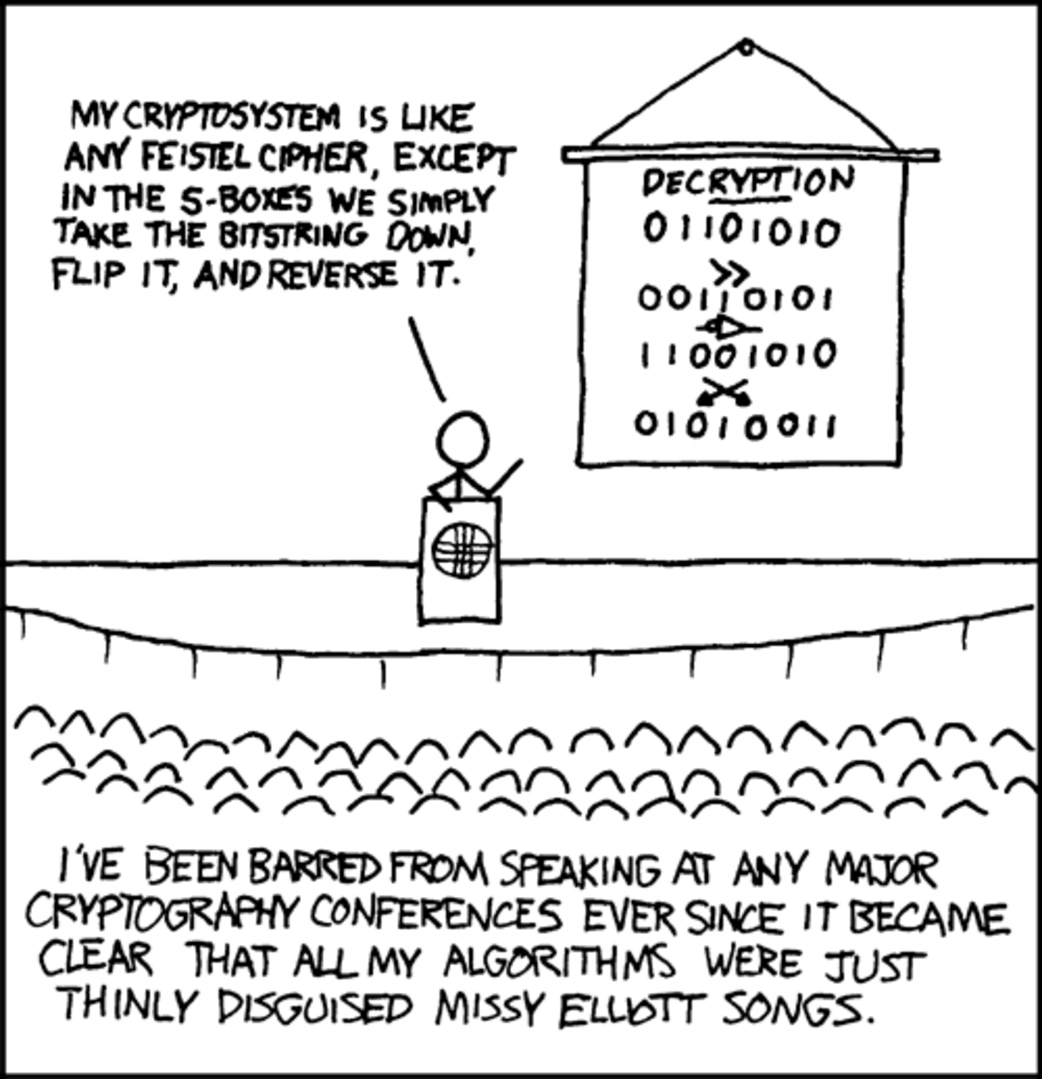
\includegraphics[width=70mm]{pic/sbox-talk} 
\end{center}
\end{figure}
\end{frame}
\begin{frame}\frametitle{Chronology of DES}
\begin{description}
\item[1973] NBS (NIST) publishes a call for a standard.
\item[1974] DES is published in the Federal Register.
\item[1977] DES is published as FIPS PUB 46.
\item[1990] Differential cryptanalysis with CPA of $2^{47}$ plaintexts. 
\item[1997] DESCHALL Project breaks DES in public.
\item[1998] EFF's Deep Crack breaks DES in 56hr at \$250,000.
\item[1999] Triple DES.
\item[2001] AES is published in FIPS PUB 197.
\item[2004] FIPS PUB 46-3 is withdrawn.
\item[2006] COPACOBANA breaks DES in 9 days at \$10,000.
\item[2008] RIVYERA breaks DES within one day.
\end{description}
\end{frame}
\begin{frame}\frametitle{AES -- The Advanced Encryption Standard}
\begin{itemize}
\item In 1997, NIST calls for AES.
\item In 2001, Rijndael [J. Daemen \& V. Rijmen] becomes AES.
\item The first publicly accessible cipher for top secret information.
\item Not only security, also efficiency and flexibility, etc.
\item 128-bit block length and 128-, 192-, or 256-bit keys.
\item Not a Feistel structure, but a SPN.
\item Only non-trivial attacks are for reduced-round variants.
\begin{itemize}
\item $2^{27}$ on 6-round of 10-round for 128-bit keys.
\item $2^{188}$ on 8-round of 12-round for 192-bit keys.
\item $2^{204}$ on 8-round of 14-round for 256-bit keys. 
\end{itemize}
\end{itemize}
\end{frame}
\begin{frame}\frametitle{Remarks on Block Ciphers}
\begin{itemize}
\item \textbf{Block length} should be sufficiently large
\item \textbf{Message tampering} is not with message confidentiality
\item \textbf{Padding}: TLS: For $n>0$, $n$ byte pad is $n,n,\dots,n$
If no pad needed, add a dummy block
\item \textbf{Stream ciphers vs. block ciphers}: 
\begin{itemize}
\item Steam ciphers are faster but have lower security
\item It is possible to use block ciphers in ``stream-cipher mode''
\end{itemize}
\end{itemize}
\begin{exampleblock}{Performance: Crypto++ 5.6, AMD Opetron 2.2GHz}
\begin{center}
\begin{tabular}{|c|c|c|} \hline
                      & \textbf{Block/key size} & \textbf{Speed MB/sec} \\ \hline
\textbf{RC4}          &         & 126 \\  
\textbf{Salsa20/12}   &         & 643 \\ 
\textbf{Sosemanuk}    &         & 727 \\ 
\textbf{3DES}	      & 64/168  & 13  \\
\textbf{AES-128}      & 128/128 & 109 \\ \hline 
\end{tabular}	
\end{center}
\end{exampleblock}
\end{frame}
\begin{frame}\frametitle{One-Way Functions (OWF)}
\begin{figure}
\begin{center}
\begin{tikzpicture}
\node (x) [circle, minimum size=1.5cm, draw] {$x$};
\node (fx) [circle, draw, right of=x, minimum size=1.5cm, node distance=4cm] {$f(x)$};

\draw[-latex,blue] (x) to [bend left=30,-latex,above] node {easy} (fx);
\draw[-latex,red] (fx) to [bend left=30,-latex,below] node {hard} (x);
\end{tikzpicture}

\end{center}
\end{figure}
The inverting experiment $\mathsf{Invert}_{\mathcal{A},f}(n)$:
\begin{enumerate}
\item Choose input $x \gets \{0,1\}^n$. Compute $y := f(x)$.
\item $\mathcal{A}$ is given $1^n$ and $y$ as input, and outputs $x'$.
\item $\mathsf{Invert}_{\mathcal{A},f}(n) = 1$ if $f(x')=y$, otherwise 0.
\end{enumerate}
\end{frame}
\begin{frame}\frametitle{Candidate One-Way Function}
\begin{itemize}
\item \textbf{Multiplication and factoring}:\\
$f_{\mathsf{mult}}(x,y)=(xy,\|x\|,\|y\|)$, $x$ and $y$ are equal-length primes.
\item \textbf{Modular squaring and square roots}:\\
$f_{\mathsf{square}}(x)=x^2\bmod N$.
\item \textbf{Discrete exponential and logarithm}:\\
$f_{g,p}(x)=g^x\bmod p$.
\item \textbf{Subset sum problem}:\\
$f(x_1,\dotsc,x_n,J)=(x_1,\dotsc,x_n,\sum_{j \in J} x_j)$.
\item \textbf{Cryptographically secure hash functions}:\\
Practical solutions for one-way computation.
\end{itemize}
\end{frame}
\begin{frame}\frametitle{Theoretical Constructions of Pseudorandom Objects}
\begin{figure}
\begin{center}
\begin{tikzpicture}[out=45,in=135]
\foreach \x / \y [evaluate=\x as \dg using \x*60] in {0/OWF,1/HCP,2/PRG,3/PRF,4/PRP,5/PrivK} {
\node (s\x) at (\dg:2.2cm) [circle, minimum size=1.5cm,draw] {\y};
}
%\foreach \x [evaluate=\x as \y using \x+1,evaluate=\x as \z using \x*60+120,evaluate=\x as \i using 300-\x*60] in {0,1,...,5} {
\foreach \x / \y in {0/1,1/2,2/3,3/4,4/5,5/0} {
\draw[-latex] (s\x) to [bend right] (s\y);
}
\end{tikzpicture}
\end{center}
\end{figure}
\begin{alertblock}{One of contributions of modern cryptography}
The existence of one-way functions is equivalent to the existence of all (non-trivial) private-key cryptography.
\end{alertblock}
\end{frame}
\begin{frame}\frametitle{Integrity and Authentication}
\begin{figure}
\begin{center}
\begin{tikzpicture}
\node (sender) [minimum size=1cm] {}; \Alice{0}{0}{0.4};
\node (bart) [below of = sender, node distance = 0.7cm] {Alice};
\node (enc) [draw, right of = sender, rounded corners=1ex,node distance = 2cm] {$\mathsf{Enc}$};
\node (k1) [above of = enc, node distance = 1cm] {$k$};
\node (c) [right of = enc, node distance = 2cm] {};
\node (gen) [draw, above of = c, rounded corners=1ex,node distance = 1cm] {$\mathsf{Gen}$};
\node (adv) [below of = c, node distance = 1cm, minimum size=1cm] {}; \Evil{4cm}{-1cm}{0.4};
\node (burns) [below of = adv, node distance = 0.7cm] {Adversary};
\node (dec) [draw, right of = c, rounded corners=1ex,node distance = 2cm] {$\mathsf{Dec}$};
\node (k2) [above of = dec, node distance = 1cm] {$k$};
\node (receiver) [right of = dec, node distance = 2cm, minimum size=1cm] {}; \Bob{8cm}{0}{0.4};
\node (lisa) [below of = receiver, node distance = 0.7cm] {Bob};
\draw[-latex] (sender) -- (enc) node [midway, above] {$m$};
\draw (enc) to node [auto,swap] {$c$} (adv); \draw[-latex] (adv) to node [auto,swap] {$c'$} (dec);
\draw[-latex] (dec) -- (receiver) node [midway, above] {$m'$};
\draw[-latex] (k1) -- (enc);
\draw[-latex] (gen) -- (k1);
\draw[-latex] (gen) -- (k2);								
\draw[-latex] (k2) -- (dec);		
\end{tikzpicture}
\begin{tikzpicture}
\node (sender) [minimum size=1cm] {}; \Alice{0}{0}{0.4};
\node (bart) [below of = sender, node distance = 0.7cm] {Alice};
\node (enc) [draw, right of = sender, rounded corners=1ex,node distance = 2cm] {$\mathsf{Enc}$};
\node (k1) [above of = enc, node distance = 1cm] {$k$};
\node (c) [right of = enc, node distance = 2cm] {};
\node (gen) [draw, above of = c, rounded corners=1ex,node distance = 1cm] {$\mathsf{Gen}$};
\node (adv) [below of = c, node distance = 1cm, minimum size=1cm] {}; \Evil{4cm}{-1cm}{0.4};
\node (burns) [below of = adv, node distance = 0.7cm] {Adversary};
\node (dec) [draw, right of = c, rounded corners=1ex,node distance = 2cm] {$\mathsf{Dec}$};
\node (k2) [above of = dec, node distance = 1cm] {$k$};
\node (receiver) [right of = dec, node distance = 2cm, minimum size=1cm] {}; \Bob{8cm}{0}{0.4};
\node (lisa) [below of = receiver, node distance = 0.7cm] {Bob};
\draw[-, dotted] (sender) -- (enc);
\draw[-, dotted] (enc) -- (dec);
\draw[-latex] (adv) to node [auto,swap] {$c'$} (dec);
\draw[-latex] (dec) -- (receiver) node [midway, above] {$m'$};
\draw[-latex] (k1) -- (enc);
\draw[-latex] (gen) -- (k1);
\draw[-latex] (gen) -- (k2);								
\draw[-latex] (k2) -- (dec);		
\end{tikzpicture}
\end{center}
\end{figure}
\end{frame}
\begin{frame}\frametitle{The Syntax of MAC}
\begin{figure}
\begin{center}
\begin{tikzpicture}[rc/.style={rounded corners=1ex, minimum width=1cm, minimum height=0.7cm}]
\node (sender) [minimum size=1cm] {}; \Alice{0}{0}{0.4};
\node (bart) [below of = sender, node distance = 0.7cm] {Alice};
\node (enc) [draw, right of = sender, rc, dotted, node distance = 2cm] {$\mathsf{Enc}$};
\node (mac) [draw, below of = enc, rc, node distance = 1.5cm] {$\mathsf{Mac}$};
\node (k1) [above of = enc, node distance = 1cm] {$k$};
\node (c) [right of = enc, node distance = 2cm] {$c$};
\node (t) [right of = mac, node distance = 2cm] {$t$};
\node (gen) [draw, above of = c, rc,node distance = 1cm] {$\mathsf{Gen}$};
%\node (adv) [below of = c, node distance = 1cm] {\Burns};
%\node (burns) [below of = adv] {Adversary};
\node (dec) [draw, right of = c, dotted,  rc,node distance = 2cm] {$\mathsf{Dec}$};
\node (ver) [draw, below of = dec, rc, node distance = 1.5cm] {$\mathsf{Vrfy}$};
\node (k2) [above of = dec, node distance = 1cm] {$k$};
\node (receiver) [right of = dec, node distance = 2cm, minimum size=1cm] {}; \Bob{8cm}{0}{0.4};
\node (lisa) [below of = receiver, node distance = 0.7cm] {Bob};
\draw[ dotted, -latex] (sender) -- (enc) node [midway, above] {$m$};
\draw[ dotted] (enc) -- (c); \draw[ dotted, -latex] (c) -- (dec);
\draw (mac) -- (t); \draw[-latex] (t) -- (ver);
\draw[ dotted, -latex] (dec) -- (receiver) node [midway, above] {$m$};
%\draw[ dotted, -latex] (k1) -- (enc);
\draw[-latex] (gen) -- (k1);
\draw[-latex] (gen) -- (k2);								
%\draw[ dotted, -latex] (k2) -- (dec);
\draw[-latex] (sender.east) -- (mac.north west) node [pos=0.7, left] {$m$};	
\draw[-latex] (ver.north east) -- (receiver.west) node [pos=0.3, right] {$b$};
\draw[-latex] (dec) -- (ver) node [midway, left] {$m$};	
\draw[-latex] (k1) -- +(1cm,-0.5cm) -- (mac.north east);
\draw[-latex] (k2) -- +(-1cm,-0.5cm) -- (ver.north west);	
\end{tikzpicture}
\end{center}
\end{figure}
\begin{itemize}
\item key $k$, tag $t$, a bit $b$ means $\mathsf{valid}$ if $b=1$; $\mathsf{invalid}$ if $b=0$.
\item \textbf{Key-generation} algorithm~$k \gets \mathsf{Gen}(1^n), \abs{k} \ge n$.
\item \textbf{Tag-generation} algorithm~$t \gets \mathsf{Mac}_k(m)$.
\item \textbf{Verification} algorithm~$b:= \mathsf{Vrfy}_k(m,t)$.
\item \textbf{Message authentication code}: $\Pi = (\mathsf{Gen}, \mathsf{Mac}, \mathsf{Vrfy})$.
\item \textbf{Basic correctness requirement}: $\mathsf{Vrfy}_k(m,\mathsf{Mac}_k(m)) = 1$.
\end{itemize}
\end{frame}
\begin{frame}\frametitle{Security of MAC}
\begin{itemize}
\item \textbf{Intuition}: No adversary should be able to generate a \textbf{valid} tag on any ``\textbf{new}'' message\footnote{A stronger requirement is concerning \emph{new message/tag pair}.} that was not previously sent.
\item \textbf{Replay attack}: Copy a message and tag previously sent. (\textbf{excluded by only considering ``new'' message})
\begin{itemize}
\item Sequence numbers: receiver must store the previous ones.
\item Time-Stamps: sender/receiver maintain synchronized clocks.
\end{itemize}
\item \textbf{Existential unforgeability}: \textbf{Not} be able to forge a valid tag on \textbf{any} message.
\begin{itemize}
\item \textbf{Existential forgery}: \emph{at least one} message.
\item \textbf{Selective forgery}: message chosen \emph{prior} to the attack.
\item \textbf{Universal forgery}: \emph{any} given message.
\end{itemize}
\item \textbf{Adaptive chosen-message attack (CMA)}: be able to obtain tags on \emph{any} message chosen adaptively \emph{during} its attack.
\end{itemize}
\end{frame}
\begin{frame}\frametitle{Definition of MAC Security}
The message authentication experiment $\mathsf{Macforge}_{\mathcal{A},\Pi }(n)$:
\begin{enumerate}
\item $k \gets \mathsf{Gen}(1^n)$.
\item $\mathcal{A}$ is given input $1^n$ and oracle access to $\mathsf{Mac}_k(\cdot)$, and outputs $(m,t)$. $\mathcal{Q}$ is the set of queries to its oracle.
\item $\mathsf{Macforge}_{\mathcal{A},\Pi }(n)=1 \iff$ $\mathsf{Vrfy}_k(m,t)=1$ $\land$ $m \notin \mathcal{Q}$. 
\end{enumerate}
\begin{figure}
\begin{center}
\begin{tikzpicture}
%\node (A) at (0,0) {\Homer};
%\node (B) [right of = A, node distance = 4cm] {\Left\Burns};
\node (A) at (0,0) [minimum size=1cm] {}; \Charlie{0}{0}{0.4};
\node (B) [right of = A, node distance = 4cm, minimum size=1cm] {}; \Evil{4cm}{0}{0.4};
\node (enc) [draw, rounded corners=1ex, right of=B, node distance = 2cm] {$\mathsf{Mac}_k(\cdot)$};
\draw[-latex] (B) to [bend left=15,-latex,above] (enc);
\draw[-latex] (enc) to [bend left=15,-latex,below] (B);
\node (k) [left of=A, node distance = 1.5cm] {Gen $k$};
\node (1a) [below of=A, node distance=1cm] {};
\node (1b) [below of=B, node distance=1cm] {$(m,t)$};
\draw[-latex] (1b) -- (1a) node [midway,above] {};
%\node (2a) [below of=1a, node distance=0.5cm] {Gen $b$};
%\node (2b) [below of=1b, node distance=0.5cm] {};
%\draw[-latex] (2b) -- (2a) node [midway,above] {};
%\node (3a) [below of=2a, node distance=0.5cm] {};
%\node (3b) [below of=2b, node distance=0.5cm] {};
%\node (4a) [below of=2a, node distance=0.5cm] {$\mathsf{Enc}_k(m_b)$};
%\node (4b) [below of=2b, node distance=0.5cm] {};
%\draw[-latex] (4a) -- (4b) node [midway,above] {};
%\node (5a) [below of=4a, node distance=0.5cm] {};
%\node (5b) [below of=4b, node distance=0.5cm] {$b'$};
%\draw[-latex] (5b) -- (5a) node [midway,above] {};
\node (6a) [below of=1a, node distance=0.5cm] {};
\node (6b) [below of=1b, node distance=0.5cm] {};
\node (result) [right of = 6a, node distance = 2cm] {Win if $\mathsf{Vrfy}_k(m,t)=1$ $\land$ $m \notin \mathcal{Q}$};
\end{tikzpicture}

\end{center}
\end{figure}
\begin{definition}
A MAC $\Pi$ is \textbf{existentially unforgeable under an adaptive CMA} if $\forall$ \textsc{ppt} $\mathcal{A}$, $\exists$ $\mathsf{negl}$ such that:
\[ \Pr [\mathsf{Macforge}_{\mathcal{A},\Pi }(n)=1] \le \mathsf{negl}(n).
\]
\end{definition}
\end{frame}
\begin{frame}\frametitle{Constructing Fixed-Length CBC-MAC}
\begin{columns}[c]
\column{.5\textwidth}
\begin{figure}
\begin{center}
\begin{tikzpicture}[scale=0.7, every node/.style={scale=0.7}]
\foreach \x in {1, 2, 3} {
\node (f\x) at ($\x*(2.5cm,0)$) [minimum size=1.25cm,rounded corners=1ex,draw] {\Large $F_k$};
\node (m\x) [above of=f\x, node distance=2.5cm] {$m_\x$};
\node (c\x) [below of=f\x, node distance=1.5cm] {$c_\x$};
\node (p\x) [above of=f\x, node distance=1.5cm, circle, draw] {};
\draw[-] (p\x.north) -- (p\x.south);
\draw[-] (p\x.east) -- (p\x.west);
\draw[-latex] (m\x) -- (p\x);
\draw[-latex] (p\x) -- (f\x);
\draw[-latex] (f\x) -- (c\x);
}

\node (iv) [left of=p1, node distance=1.5cm] {$IV$};
\node (iv2) [left of=c1, node distance=1.5cm] {$IV$};
\draw[-latex] (iv) -- (iv2);
\draw[-latex] (iv) -- (p1);

\foreach \x in {1, 2} {
\draw[-latex] ($(c\x) + (0,0.6cm)$) -| +(1.25cm,2.4cm) -- ($(p\x.west) + (2.5cm,0)$);
}

\end{tikzpicture}
\end{center}
\end{figure}
\column{.5\textwidth}
\begin{figure}
\begin{center}
\begin{tikzpicture}[scale=0.7, every node/.style={scale=0.7}]
\foreach \x in {1, 2, 3} {
\node (f\x) at ($\x*(2.5cm,0)$) [minimum size=1.25cm,rounded corners=1ex,draw] {\Large $F_k$};
\node (m\x) [above of=f\x, node distance=2cm] {$m_\x$};
\node (p\x) [above of=f\x, node distance=1.2cm, circle, draw] {};
\draw[-] (p\x.north) -- (p\x.south);
\draw[-] (p\x.east) -- (p\x.west);
\draw[-latex] (m\x) -- (p\x);
\draw[-latex] (p\x) -- (f\x);
}

\foreach \x in {1, 2} {
\draw[-latex] (f\x.south) -- +(0cm,-0.3cm) -| +(1.25cm,1.85cm) -- ($(p\x.west) + (2.5cm,0)$);
}
\node (m) [left of=p1, node distance = 1cm] {$0^n$};
\draw[-latex] (m) -- (p1);
\draw[-latex] (f3.south) |- +(0.5cm,-0.3cm) node [anchor=west] {t}; 
\end{tikzpicture}
\end{center}
\end{figure}
\end{columns}
Modify CBC encryption into CBC-MAC:
\begin{itemize}
\item Change random $IV$ to encrypted fixed $0^{n}$,\emph{otherwise}:\\
\alert{Q: query $m_1$ and get $(IV, t_1)$; output $m_1' = IV' \oplus  IV \oplus m_{1}$ and $t' =$ \underline{$\qquad $}.} %(IV',t_1)$.
\item Tag only includes the output of the final block,\emph{otherwise}:\\
\alert{Q: query $m_i$ and get $t_i$; output $m_i' = t_{i-1}' \oplus t_{i-1} \oplus m_{i}$ and $t_{i}' = $ \underline{$\qquad$}.}%$t_i$.
\end{itemize}
\end{frame}
\begin{frame}\frametitle{Secure Variable-Length MAC}
\begin{itemize}
\item \textbf{Input-length key separation}: $k_{\ell} := F_k(\ell)$, use $k_{\ell}$ for CBC-MAC.
\item \textbf{Length-prepending}: Prepend $m$ with $|m|$, then use CBC-MAC.
\begin{figure}
\begin{center}
\begin{tikzpicture}[scale=0.7, every node/.style={scale=0.7}]
\foreach \x in {1, 2, 3, 4} {
\node (f\x) at ($\x*(2.5cm,0)$) [minimum size=1.25cm,rounded corners=1ex,draw] {\Large $F_k$};
}
\node (p1) [above of=f1, node distance=1.2cm] {};
\foreach \x/\y in {2/1,3/2,4/3} {
\node (m\x) [above of=f\x, node distance=2cm] {$m_\y$};
\node (p\x) [above of=f\x, node distance=1.2cm, circle, draw] {};
\draw[-] (p\x.north) -- (p\x.south);
\draw[-] (p\x.east) -- (p\x.west);
\draw[-latex] (m\x) -- (p\x);
\draw[-latex] (p\x) -- (f\x);
}

\foreach \x in {1, 2, 3} {
\draw[-latex] (f\x.south) -- +(0cm,-0.3cm) -| +(1.25cm,1.85cm) -- ($(p\x.west) + (2.5cm,0)$);
}
\node (m) [above of=f1, node distance = 2cm] {$|m|$};
\draw[-latex] (m) -- (f1);
\draw[-latex] (f4.south) |- +(0.5cm,-0.3cm) node [anchor=west] {t}; 
\end{tikzpicture}
\end{center}
\end{figure}
\item \textbf{Encrypt last block (ECBC-MAC)}: Use two keys $k_1, k_2$. Get $t$ with $k_1$ by CBC-MAC, then output $\hat{t} := F_{k_2}(t)$.
\end{itemize}
\alert{Q: To authenticate a voice stream, which approach do you prefer?}
\end{frame}
\begin{frame}\frametitle{Weaker Notions of Security for Hash Functions}
\begin{figure}
\begin{center}
\begin{tikzpicture}[uk/.style={inner sep=1pt, minimum width=10pt, circle, fill=red!50},kk/.style={inner sep=1pt, minimum width=10pt, fill=blue!50, circle}]
\foreach \i in {1, 2, 3} {
\node (X\i) at (\i*4cm,0) [ellipse,minimum width=1cm,minimum height=2cm,draw] {}; 
\node (x) [above of=X\i,node distance=1.2cm] {$X$}; 
\node (Y\i) [right of=X\i,ellipse,minimum width=1cm,minimum height=2cm,node distance=1.5cm,draw] {};
\node (y) [above of=Y\i,node distance=1.2cm] {$Y$}; 
}
\node (cr) at ($(X1)+(0.75cm,-1.5cm)$) [] {\footnotesize Collision};
\node (cr) at ($(X1)+(0.75cm,-1.8cm)$) [] {\footnotesize Resistance};
\node (x1) at ($(X1)+(0,0.3cm)$) [uk] {\tiny ?};
\node (x2) at ($(X1)+(0,-0.3cm)$) [uk] {\tiny ?};
\node (y1) at ($(Y1)$) [uk] {\tiny ?};
\draw[-latex] (x1) -- (y1);
\draw[-latex] (x2) -- (y1);
\node (2pr) at ($(X2)+(0.75cm,-1.5cm)$) [] {\footnotesize 2nd Pre-image};
\node (2pr) at ($(X2)+(0.75cm,-1.8cm)$) [] {\footnotesize Resistance};
\node (x1) at ($(X2)+(0,0.3cm)$) [kk] {\tiny x};
\node (x2) at ($(X2)+(0,-0.3cm)$) [uk] {\tiny ?};
\node (y1) at ($(Y2)$) [kk] {\tiny y};
\draw[-latex] (x1) -- (y1);
\draw[-latex] (x2) -- (y1);
\node (pr) at ($(X3)+(0.75cm,-1.5cm)$) [] {\footnotesize Pre-image};
\node (pr) at ($(X3)+(0.75cm,-1.8cm)$) [] {\footnotesize Resistance};
%\node (x1) at ($(X3)+(0,0.3cm)$) [kk] {\tiny x};
\node (x2) at ($(X3)+(0,-0.3cm)$) [uk] {\tiny ?};
\node (y1) at ($(Y3)$) [kk] {\tiny y};
%\draw[-latex] (x1) -- (y1);
\draw[-latex] (x2) -- (y1);
\end{tikzpicture}

\end{center}
\end{figure}
\begin{itemize}
\item \textbf{Collision resistance}: It is hard to find $(x, x'), x' \ne x$ such that $H(x) = H(x')$.
\item \textbf{Second pre-image resistance}: Given $s$ and $x$, it is hard to find $x' \ne x$ such that $H^s(x') = H^s(x)$.
\item \textbf{Pre-image resistance}: Given $s$ and $y = H^s(x)$, it is hard to find $x'$ such that $H^s(x')=y$.
\end{itemize}
\end{frame}
\begin{frame}{Applications of Hash Functions}
\begin{itemize}
\item \textbf{Fingerprinting and Deduplication}: $H(alargefile)$ for virus fingerprinting, deduplication, P2P file sharing
\item \textbf{Merkle Trees}: $H(H(H(file1), H(file2)), H(H(file3), H(file4)))$ fingerprinting multiple files / parts of a file
\item \textbf{Passward Hashing}: $(salt, H(salt, pw))$ mitigating the risk of leaking password stored in the clear 
\item \textbf{Key Derivation}: $H(secret)$ deriving a key from a high-entropy (but not necessarily uniform) shared secret
\item \textbf{Commitment Schemes}: $H(info)$ hiding the commited info; binding the commitment to a info
\end{itemize}
\end{frame}
\begin{frame}\frametitle{Hash-based MAC (HMAC)}
\begin{figure}
\begin{center}
\begin{tikzpicture}[cf/.style={trapezium left angle=65, trapezium right angle=90, minimum height=1cm,minimum width=1cm,trapezium, rounded corners=1ex,shape border rotate=270, draw}]
\foreach \i in {1,2,...,6} {
\ifnum \i = 3
\node (h\i) at ($\i*(1.5cm,0)$) [trapezium left angle=65, trapezium right angle=90, minimum height=1cm,minimum width=1cm,trapezium, rounded corners=1ex,shape border rotate=270] {$\cdots$};
\else
\node (h\i) at ($\i*(1.5cm,0)$) [cf] {$h^s$};
\fi
}
\foreach \i/\j in {1/2,2/3,3/4,4/5,5/6} {
\ifnum \i = 3
\node (x\i) at ($\i*(1.5cm,0)+(0,1.5cm)$) [minimum height=0.6cm, minimum width=1.5cm] {$\cdots$};
\else
\ifnum \i = 4
\node (x\i) at ($\i*(1.5cm,0)+(0,1.5cm)$) [minimum height=0.6cm, minimum width=1.5cm] {$|m|$};
\else
\ifnum \i = 5
\node (x\i) at ($\i*(1.5cm,0)+(0.9cm,1.5cm)$) [minimum height=0.6cm, minimum width=1.5cm] {$k\oplus opad$};
\node (iv2) at ($\i*(1.5cm,0)+(-0.5cm,1.5cm)$) [minimum height=0.6cm, minimum width=1.5cm] {$IV$};
\draw [-latex] (iv2) -- (h\i);
\else
\ifnum \i = 1
\node (x\i) at ($\i*(1.5cm,0)+(0,1.5cm)$) [minimum height=0.6cm, minimum width=1.5cm] {$k\oplus ipad$};
\else
\ifnum \i = 2
\node (x\i) at ($\i*(1.5cm,0)+(0,1.5cm)$) [minimum height=0.6cm, minimum width=1.3cm,draw] {$m_{1}$};
\else
\node (x\i) at ($\i*(1.5cm,0)+(0,1.5cm)$) [minimum height=0.6cm, minimum width=1.5cm,draw] {$k\oplus opad$};
\fi
\fi
\fi
\fi
\draw[-latex] (x\i) -- (h\i);
\fi
\ifnum \i = 4 
\draw[-latex] (h4) -| +(0.75cm,-0.7) -- +(2.1cm,-0.7) |- ($(h6.west)+(0,-0.1cm)$);
\else
\ifnum \i = 5
\draw[-latex] ($(h5.east)+(0,0.3cm)$) -- ($(h6.west)+(0,0.3cm)$);
\else 
\draw[-latex] (h\i) -- (h\j);
\fi
\fi
}
\node (iv) at (0.2cm,0) {$IV$};
\node (hs) at (10.1cm,0) {$t$};
\draw[-latex] (iv) -- (h1);
\draw[-latex] (h6) -- (hs);
\end{tikzpicture}
\end{center}
\end{figure}
\begin{construction}
$(\widetilde{\mathsf{Gen}}, h)$ is a fixed-length CRHF. $(\widetilde{\mathsf{Gen}}, H)$ is the Merkle-Damg\r{a}rd transform.
$IV$, $\mathsf{opad}$ (0x36), $\mathsf{ipad}$ (0x5C) are fixed constants of length $n$.
HMAC:
\begin{itemize}
\item $\mathsf{Gen}(1^n)$: Output $(s, k)$. $s \gets \widetilde{\mathsf{Gen}}, k \gets \{0,1\}^n$ \emph{u.a.r}
\item $\mathsf{Mac}_{s,k}(m)$: $t := H_{IV}^s\Big((k \oplus \mathsf{opad}) \| H_{IV}^s\big((k \oplus \mathsf{ipad}) \| m\big)\Big)$
\item $\mathsf{Vrfy}_{s,k}(m,t)$: $1 \iff t \overset{?}{=} \mathsf{Mac}_{s,k}(m)$
\end{itemize}
\end{construction}
\end{frame}
\begin{frame}\frametitle{Security of HMAC}
\begin{theorem}
\[ G(k) \overset{\text{def}}{=} h^s(IV\| (k\oplus \mathsf{opad})) \| 
h^s(IV\| (k\oplus \mathsf{ipad})) = k_1\| k_2
\]
$(\widetilde{\mathsf{Gen}}, h)$ is CRHF. If $G$ is a PRG, then HMAC is secure.
\end{theorem}
\begin{itemize}
\item HMAC is an industry standard (RFC2104)
\item HMAC is faster than CBC-MAC
\item Before HMAC, a common mistake was to use $H^s(k\| x)$
\item \alert{Verification timing attacks: (Keyczar crypto library (Python))} \\
def Verify(key, msg, sig\underline{\ }bytes): \\
$\qquad$ return HMAC(key, msg) == sig\underline{\ }bytes \\
The problem:  implemented as a byte-by-byte comparison
\item \alert{\emph{Don't implement it yourself}}
\end{itemize}
\end{frame}
\begin{frame}\frametitle{Combining Encryption and Authentication}
\begin{figure}
\begin{center}
\begin{tikzpicture}
\node (enc1) [minimum width=1.5cm, minimum height=1.5cm, draw] {$\mathsf{Enc}$};
\node (mac1) [right of=enc1, minimum width=1.5cm, minimum height=1.5cm, node distance=1.5cm, draw] {$\mathsf{Mac}$};	

\node (enc2) [right of=mac1, node distance=3cm, minimum width=3cm, minimum height=1.5cm, draw] {};
\node (mac2) [right of=enc2, minimum width=1.5cm, minimum height=1cm, node distance=0.75cm, draw] {$\mathsf{Mac}$};
\node (enc4) [left of=enc2, minimum width=1cm, minimum height=1cm, node distance=0.75cm] {$\mathsf{Enc}$}; 

\node (mac3) [right of=mac2, node distance=3cm, minimum width=3cm, minimum height=1.5cm, draw] {};
\node (enc3) [right of=mac3, minimum width=1.5cm, minimum height=1cm, node distance=0.75cm, draw] {$\mathsf{Enc}$};
\node (enc5) [left of=mac3, minimum width=1cm, minimum height=1cm, node distance=0.75cm] {$\mathsf{Mac}$};	
\end{tikzpicture}
\end{center}
\end{figure}
\begin{itemize}
\item \textbf{Encrypt-and-authenticate} (e.g., SSH):\[ c \gets \mathsf{Enc}_{k_1}(m),\; t \gets \mathsf{Mac}_{k_2}(m).\]
\item \textbf{Authenticate-then-encrypt} (e.g, SSL):\[ t \gets \mathsf{Mac}_{k_2}(m),\; c \gets \mathsf{Enc}_{k_1}(m\| t).\]
\item \textbf{Encrypt-then-authenticate} (e.g, IPsec):\[ c \gets \mathsf{Enc}_{k_1}(m),\; t \gets \mathsf{Mac}_{k_2}(c). \]
\end{itemize}
\end{frame}
\begin{frame}\frametitle{Analyzing Security of Combinations}
\textbf{All-or-nothing}: Reject any combination for which there exists even a single counterexample is insecure.
\begin{itemize}
\item \textbf{Encrypt-and-authenticate}: $\mathsf{Mac}'_k(m) = (m, \mathsf{Mac}_k(m))$.
\item \textbf{Authenticate-then-encrypt}: 
\begin{itemize}
\item $\mathsf{Trans}: 0 \to 00; 1 \to 10/01$; $\mathsf{Enc}'$ uses CTR mode; $c = \mathsf{Enc}'(\mathsf{Trans}(m\| \mathsf{Mac}(m)))$.
\item Flip the first two bits of $c$ and verify whether the ciphertext is valid.
$10/01 \to 01/10 \to 1$, $00 \to 11 \to \bot$.
\item If valid, the first bit of message is 1; otherwise 0.\\
\item For any MAC, this is not CCA-secure.
\end{itemize}
\item \textbf{Encrypt-then-authenticate}: \\
Decryption: If $\mathsf{Vrfy}(\cdot) = 1$, then $\mathsf{Dec}(\cdot)$; otherwise output $\bot$.
\end{itemize}
\end{frame}
\begin{frame}\frametitle{Authenticated Encryption Theory and Practice}
\begin{theorem}
$\Pi_E$ is CPA-secure and $\Pi_E$ is a secure MAC with unique tages, $\Pi'$ deriving from encrypt-then-authenticate approach is secure.
\end{theorem}
\textbf{GCM(Galois/Counter Mode)}: CTR encryption then Galois MAC. (RFC4106/4543/5647/5288 on IPsec/SSH/TLS)\\
\textbf{EAX}: CTR encryption then CMAC.
\begin{proposition}
Authenticate-then-encrypt approach is secure if $\Pi_E$ is rand-CTR mode or rand-CBC mode.
\end{proposition}
\textbf{CCM (Counter with CBC-MAC)}: CBC-MAC then CTR encryption. (802.11i, RFC3610)\\
\textbf{OCB (Offset Codebook Mode)}: integrating MAC into ENC. (two times fast as CCM, EAX)\\
\textbf{All support AEAD (A.E. with associated data):} part of message is in clear, and all is authenticated
\end{frame}
\begin{frame}\frametitle{Remarks on Secure Message Transmission}
\begin{itemize}
\item Authentication may leak the message.
\item Secure message transmission implies CCA-security. The opposite direction is not necessarily true.
\item Different security goals should always use different keys.
\begin{itemize}
\item otherwise, the message may be leaked if $\mathsf{Mac}_k(c)=\mathsf{Dec}_k(c)$.
\end{itemize}
\item Implementation may destroy the security proved by theory.
\begin{itemize}
\item \textbf{Attack with padding oracle} (in TLS 1.0): \\
\textbf{Dec} return two types of error: padding error, MAC error. \\
\textbf{Adv.} learns last bytes if no padding error with guessed bytes. 
\item \textbf{Attack non-atomic dec.} (in SSH Binary Packet Protocol):\\
\textbf{Dec} (1)decrypt length field; (2)read packets as specified by the length; (3)check MAC. \\
\textbf{Adv.} (1)send $c$; (2)send $l$ packets until ``MAC error'' occurs; (3)learn $l = \mathsf{Dec}(c)$. 
\end{itemize}
\end{itemize}
\end{frame}
\begin{frame}\frametitle{ Password-Based KDF (PBKDF)}
\textbf{Key stretching} increases the time of testing key (with slow hash function).
\newline

\textbf{Key strengthening} increases the length/randomness of key (with salt).
\newline

\textbf{PKCS\#5 (PBKDF1)}: $H^{(c)}(pwd\|salt)$, iterate hash function $c$ times.
\newline

\textbf{Attack}: either try the enhanced key (larger key space), or else try the initial key (longer time per key).
\end{frame}
\begin{frame}\frametitle{Public-Key Revolution}
\begin{itemize}
\item In 1976, Whitfield Diffie and Martin Hellman published ``\emph{New Directions in Cryptography}''.
\item \textbf{Asymmetric} or \textbf{public-key} encryption schemes:
\begin{itemize}
\item \textbf{Public key} as the encryption key.
\item \textbf{Private key} as the decryption key.
\end{itemize}
\item \textbf{Public-key primitives}:
\begin{itemize}
\item Public-key encryption.
\item Digital signatures. (non-repudiation)
\item Interactive key exchange.
\end{itemize}
\item \textbf{Strength}:
\begin{itemize}
\item Key distribution over public channels.
\item Reduce the need to store many keys.
\item Enable security in open system.
\end{itemize}
\item \textbf{Weakness}: slow, active attack on public key distribution.
%\item \textbf{Peoples}: Ralphe Merkle (his advisor at Stanford was Hellman), Michael Rabin, Rivest, Shamir, and Adleman.
\end{itemize}
\end{frame}
\begin{frame}\frametitle{Definitions}
\begin{figure}
\begin{center}
\begin{tikzpicture}
\node (sender) [minimum size=1cm] {}; \Alice{0}{0}{0.4};
\node (bart) [below of = sender, node distance = 0.7cm] {Alice};
\node (enc) [draw, right of = sender, rounded corners=1ex,node distance = 2cm] {$\mathsf{Enc}$};
\node (k1) [above of = enc, node distance = 1cm] {$pk$};
\node (c) [right of = enc, node distance = 2cm] {$c$};
\node (gen) [draw, above of = c, rounded corners=1ex,node distance = 1cm] {$\mathsf{Gen}$};
\node (adv) [below of = c, node distance = 1cm, minimum size=1cm] {}; \Evil{4cm}{-1cm}{0.4};
\node (burns) [below of = adv, node distance = 0.7cm] {Adversary};
\node (dec) [draw, right of = c, rounded corners=1ex,node distance = 2cm] {$\mathsf{Dec}$};
\node (k2) [above of = dec, node distance = 1cm] {$sk$};
\node (receiver) [right of = dec, node distance = 2cm, minimum size=1cm] {}; \Bob{8cm}{0}{0.4};
\node (lisa) [below of = receiver, node distance = 0.7cm] {Bob};
\draw[-latex] (sender) -- (enc) node [midway, above] {$m$};
\draw (enc) -- (c); \draw[-latex] (c) -- (dec);
\draw[-latex] (dec) -- (receiver) node [midway, above] {$m$};
\draw[-latex] (k1) -- (enc);
\draw[-latex] (gen) -- (k1);
\draw[-latex] (gen) -- (k2);								
\draw[-latex] (k2) -- (dec);
\draw[-latex, dotted] (k1) -- (adv);		
\end{tikzpicture}
\end{center}
\end{figure}
\begin{itemize}
\item \textbf{Key-generation} algorithm: $(pk,sk) \gets \mathsf{Gen}$, key length $\ge n$.
\item  \textbf{Plaintext space} $\mathcal{M}$ is associated with $pk$.
\item \textbf{Encryption} algorithm: $c \gets \mathsf{Enc}_{pk}(m)$.
\item \textbf{Decryption} algorithm: $m:= \mathsf{Dec}_{sk}(c)$, or outputs $\perp$.
\item \textbf{Requirement}: $\Pr[\mathsf{Dec}_{sk}(\mathsf{Enc}_{pk}(m)) = m] \ge 1 - \mathsf{negl}(n)$.
\end{itemize}
\end{frame}
\begin{frame}\frametitle{Construction of Hybrid Encryption}
To speed up the encryption of long message, use private-key encryption $\Pi'$ in tandem with public-key encryption $\Pi$.
\begin{columns}
\begin{column}{5cm}
\begin{figure}
\begin{center}
\begin{tikzpicture}
\node (f1) [minimum size=1.25cm,rounded corners=1ex,draw] {$\mathsf{Enc}_{pk}$};
\node (f2) at (2.5cm,0) [minimum size=1.25cm,rounded corners=1ex,draw] {$\mathsf{Enc}'_{k}$};
\draw[-latex] (0,1.5cm) node [above] {$k$} -- (f1);
\draw[-latex] (2.5,1.5cm) node [above] {$m$} -- (f2);
\draw[-latex] (-1cm,0) node [left] {$pk$} -- (f1);
\draw[-latex] (f1) -- +(0,-1.5) node [below] {$c_1$};
\draw[-latex] (f2) -- +(0,-1.5) node [below] {$c_2$};
\draw[-latex] (0,1.25) -| (1.25,0) -- (f2);
\end{tikzpicture}
\end{center}
\end{figure}
\end{column}
\begin{column}{5cm}
\begin{construction}
$\Pi^{\mathsf{hy}} = (\mathsf{Gen}^{\mathsf{hy}}, \mathsf{Enc}^{\mathsf{hy}}, \mathsf{Dec}^{\mathsf{hy}})$:
\begin{itemize}
\item $\mathsf{Gen}^{\mathsf{hy}}$: $(pk,sk) \gets \mathsf{Gen}(1^n)$.
\item $\mathsf{Enc}^{\mathsf{hy}}$: $pk$ and $m$. 
\begin{enumerate}
\item $k \gets \{0,1\}^n$.
\item $c_1 \gets \mathsf{Enc}_{pk}(k)$, $c_2 \gets \mathsf{Enc}'_{k}(m)$.
\end{enumerate}
\item $\mathsf{Dec}^{\mathsf{hy}}$: $sk$ and $\langle c_1,c_2\rangle$.
\begin{enumerate}
\item $k := \mathsf{Dec}_{sk}(c_1)$.
\item $m := \mathsf{Dec}'_k(c_2)$.
\end{enumerate}
\end{itemize}
\end{construction}
\end{column}
\end{columns}
\alert{Q: is hybrid encryption a public-key enc. or private-key enc. ?}
\end{frame}
\begin{frame}\frametitle{Trapdoor Permutations}
\textbf{Trapdoor function}: is easy to compute, yet difficult to find its inverse without special info., the ``trapdoor''. (One Way Function with the ``trapdoor'')
\newline

A public-key encryption scheme can be constructed from any trapdoor permutation. (``\emph{Theory and Applications of Trapdoor Functions}'', [Yao, 1982])
\begin{figure}
\begin{center}
\begin{tikzpicture}
\node (x) [circle, minimum size=1.5cm, draw] {$x$};
\node (fx) [circle, draw, right of=x, minimum size=1.5cm, node distance=4cm] {$f(x)$};
\node (hc) at ($(x)+(2cm,-1cm)$) [circle, draw] {$\mathsf{hc}(x)$};
\node (tp) [draw, right of=x, node distance=2cm] {$\mathsf{tp}$};
\node (ez) [above of=tp, node distance=0.5cm, blue] {easy};

\draw[-latex,blue] (x) to [bend left=30,-latex,above] node {easy} (fx);
\draw[-latex,red] (fx) to [bend left=30,-latex,right] node {hard} (hc);
\draw[-latex,blue] (x) to [bend right=30,-latex,left] node {easy} (hc);
\draw[-latex,blue] (fx) -- (tp)  -- (x);
\draw[-latex,red] (fx) to [bend right=-120,-latex,below] node {hard} (x);
\end{tikzpicture}
\end{center}
\end{figure}
\end{frame}
\begin{frame}\frametitle{Public-key Encryption Schemes from TDPs}
\begin{construction}
\begin{itemize}
\item $\mathsf{Gen}$: $(I, \mathsf{td}) \gets \widehat{Gen}$ output \textbf{public key} $I$ and \textbf{private key} $\mathsf{td}$.
\item $\mathsf{Enc}$: on input $I$ and $m \in \{0,1\}$, choose a random $x\gets \mathcal{D}_I$ and output $\langle f_I(x), \mathsf{hc}_I(x)\oplus m \rangle$.
\item $\mathsf{Dec}$: on input $\mathsf{td}$ and $\langle y, m'\rangle$, compute $x:= f^{-1}_I(y)$ and output $\mathsf{hc}_I(x)\oplus m'$.
\end{itemize}
\end{construction}
\begin{theorem}
If $\widehat{\Pi}=(\widehat{Gen},f)$ is TDP, and $\mathsf{hc}$ is HCP for $\widehat{\Pi}$, then Construction $\Pi$ is CPA-secure.
\end{theorem}
\begin{exampleblock}{Is the following scheme is secure?}
$\mathsf{Enc}_{I}(m) = f_I(m)$, $\mathsf{Dec}_{\mathsf{td}}(c) = f^{-1}_I(c)$.
\end{exampleblock}
\end{frame}
\begin{frame}\frametitle{Scenarios of CCA in Public-Key Setting}
\begin{enumerate}
\item An adversary $\mathcal{A}$ observes the ciphertext $c$ sent by $\mathcal{S}$ to $\mathcal{R}$.
\item $\mathcal{A}$ send $c'$ to $\mathcal{R}$ in the name of $\mathcal{S}$ or its own.
\item $\mathcal{A}$ infer $m$ from the decryption of $c'$ to $m'$.
\end{enumerate}
\begin{exampleblock}{Scenarios}
\begin{itemize}
\item \textbf{login to on-line bank with the password}: trial-and-error, learn info from the feedback of bank.
\item \textbf{reply an e-mail with the quotation of decrypted text}.
\item \textbf{malleability of ciphertexts}: e.g. doubling others' bids at an auction.
\end{itemize}
\end{exampleblock}
\end{frame}
\begin{frame}{State of the Art on CCA2-secure Encryption}
\begin{itemize}
\item \textbf{Zero-Knowledge Proof}: complex, and impractical. (e.g., Dolev-Dwork-Naor)
\item \textbf{Random Oracle} model: efficient, but not realistic (to consider CRHF as RO). (e.g., RSA-OAEP and Fujisaki-Okamoto)
\item \textbf{DDH(Decisional Diffie-Hellman assumption) and UOWHF(Universal One-Way Hashs Function)}: x2 expansion in size, but security proved w/o RO or ZKP (e.g., Cramer-Shoup system).
\end{itemize}
\textbf{CCA2-secure implies Plaintext-aware}: an adversary cannot produce a valid ciphertext without ``knowing'' the plaintext.
\begin{block}{Open problem}
Constructing a CCA2-secure scheme based on RSA problem as efficient as ``Textbook RSA''.
\end{block}
\end{frame}
\begin{frame}\frametitle{Private Key Encryption vs. Public Key Encryption}
\begin{center}
\begin{tabular}{|c|c|c|} \hline
   & \textbf{Private Key} & \textbf{Public Key}             \\ \hline
\textbf{Secret Key}               & both parties & receiver \\ \hline
\textbf{Weakest Attack}           & Eav          & CPA      \\ \hline
\textbf{Probabilistic}            & CPA/CCA      & always   \\ \hline
\textbf{Assumption against CPA}   & OWF          & TDP      \\ \hline
\textbf{Assumption against CCA}   & OWF          & TDP$+$RO   \\ \hline
\textbf{Efficiency}               & fast         & slow     \\ \hline
\end{tabular}	
\end{center}
\end{frame}
\begin{frame}\frametitle{RSA Overview}
\begin{itemize}
\item \textbf{RSA}: Ron Rivest, Adi Shamir and Leonard Adleman, in 1977
\item \textbf{RSA problem}: Given $N = pq$ (two distinct big prime numbers) and $y \in \mathbb{Z}^*_N$, compute $y^{-e}$, $e^{\text{th}}$-root of $y$ modulo $N$
\item \alert{Open problem}:RSA problem is easier than factoring $N$?
\item \textbf{Certification}: PKCS\#1 (RFC3447), ANSI X9.31, IEEE 1363
\item \textbf{Key sizes}: 1,024 to 4,096 bit
\item \textbf{Best public cryptanalysis}: a 768 bit key has been broken
\item \textbf{RSA Challenge}: break RSA-2048 to win \$200,000 USD
\end{itemize}
\textbf{Key lengths} with comparable security :
\begin{center}
\begin{tabular}{|c|c|} \hline
Symmetric & RSA  \\ \hline
80 bits & 1024 bits   \\
128 bits & 3072 bits  \\
256 bits & 15360 bits \\ \hline
\end{tabular}	
\end{center}
\end{frame}
\begin{frame}\frametitle{``Textbook RSA''}
\begin{construction}
\begin{itemize}
\item $\mathsf{Gen}$: on input $1^n$ run $\mathsf{GenRSA}(1^n)$ to obtain $N,e,d$. $pk = \langle N,e \rangle$ and $sk = \langle N,d \rangle$.
\item $\mathsf{Enc}$: on input $pk$ and $m \in \mathbb{Z}^*_N$, $c:= [m^e \bmod N]$.
\item $\mathsf{Dec}$: on input $sk$ and $m \in \mathbb{Z}^*_N$, $m:= [c^d \bmod N]$.
\end{itemize}
\end{construction}
\begin{alertblock}{Insecurity}
Since the ``textbook RSA'' is deterministic, it is insecure with respect to any of the definitions of security we have proposed. 
\end{alertblock}
\end{frame}
\begin{frame}\frametitle{PKCK \#1 v2.1 (RSAES-OAEP) (Cont.)}
RSA-OAEP is CCA-secure in Random Oracle model. \footnote{It may not be secure when RO is instantiated.} [RFC 3447]
\begin{figure}
\begin{center}
\begin{tikzpicture}[scale=0.8, every node/.style={scale=0.8}]
\node (m) [draw,minimum width=1.5cm, minimum height=0.5cm] {$m$};
\node (p0) at (2cm,0) [draw, minimum width=1.5cm, minimum height=0.5cm] {$00\cdots 0$};
\node (r) at (4.5cm,0) [draw,minimum width=3cm, minimum height=0.5cm] {$r$};

\node (xor) at (1cm,-1cm) [circle, draw] {};
\draw[-] (xor.north) -- (xor.south);
\draw[-] (xor.east) -- (xor.west);
\node (xor2) at (4.5cm,-2cm) [circle, draw] {};
\draw[-] (xor2.north) -- (xor2.south);
\draw[-] (xor2.east) -- (xor2.west);

\node (G) at (2.75cm,-1cm) [draw,rounded corners=1ex] {$G$};
\node (H) at (2.75cm,-2cm) [draw,rounded corners=1ex] {$H$};

\node (m1) at (1cm,-3cm) [draw,minimum width=3cm, minimum height=0.5cm] {$s$};
\node (mh) at (4.5cm,-3cm) [draw,minimum width=3cm, minimum height=0.5cm] {$t$};

\draw [-] (m) |- (1cm,-0.5cm);
\draw [-] (p0) |- (1cm,-0.5cm) -- (xor);
\draw [-] (xor) -- (G);
\draw [-latex] (r) |- (G);
\draw [-latex] (xor) |- (H);
\draw [-] (r) |- (H);
\draw [-latex] (xor) -- (m1);
\draw [-latex] (xor2) -- (mh);
\end{tikzpicture}
\end{center}
\end{figure}
CPA: To learn $r$, attacker has to learn $\hat{m}_1$ from $(\hat{m}_1\|\hat{m})^e$\\

CCA: Effective decryption query is disabled by checking "00...0" in the plaintext before the response\\

\end{frame}

\begin{frame}\frametitle{OAEP Improvements}
\begin{columns}
\begin{column}{5cm}
\begin{figure}
\begin{center}
\begin{tikzpicture}[scale=0.8, every node/.style={scale=0.8}]
\node (m) [draw,minimum width=1.5cm, minimum height=0.5cm] {$m$};
\node (p0) at (2cm,0) [draw, minimum width=1.5cm, minimum height=0.5cm] {$W(m,r)$};
\node (r) at (4.5cm,0) [draw,minimum width=3cm, minimum height=0.5cm] {$r$};

\node (xor) at (1cm,-1cm) [circle, draw] {};
\draw[-] (xor.north) -- (xor.south);
\draw[-] (xor.east) -- (xor.west);
\node (xor2) at (4.5cm,-2cm) [circle, draw] {};
\draw[-] (xor2.north) -- (xor2.south);
\draw[-] (xor2.east) -- (xor2.west);

\node (G) at (2.75cm,-1cm) [draw,rounded corners=1ex] {$G$};
\node (H) at (2.75cm,-2cm) [draw,rounded corners=1ex] {$H$};

\node (m1) at (1cm,-3cm) [draw,minimum width=3cm, minimum height=0.5cm] {$\hat{m}_1$};
\node (mh) at (4.5cm,-3cm) [draw,minimum width=3cm, minimum height=0.5cm] {$\hat{m}$};

\draw [-] (m) |- (1cm,-0.5cm);
\draw [-] (p0) |- (1cm,-0.5cm) -- (xor);
\draw [-] (xor) -- (G);
\draw [-latex] (r) |- (G);
\draw [-latex] (xor) |- (H);
\draw [-] (r) |- (H);
\draw [-latex] (xor) -- (m1);
\draw [-latex] (xor2) -- (mh);
\end{tikzpicture}
\begin{tikzpicture}[scale=0.8, every node/.style={scale=0.8}]
\node (m) [draw,minimum width=1.5cm, minimum height=0.5cm] {$m$};
\node (p0) at (2cm,0) [draw, minimum width=1.5cm, minimum height=0.5cm] {$W(m,r)$};
\node (r) at (4.5cm,0) [draw,minimum width=3cm, minimum height=0.5cm] {$r$};

\node (xor) at (1cm,-1cm) [circle, draw] {};
\draw[-] (xor.north) -- (xor.south);
\draw[-] (xor.east) -- (xor.west);
%\node (xor2) at (4.5cm,-2cm) [circle, draw] {};
%\draw[-] (xor2.north) -- (xor2.south);
%\draw[-] (xor2.east) -- (xor2.west);

\node (G) at (2.75cm,-1cm) [draw,rounded corners=1ex] {$H$};
%\node (H) at (2.75cm,-2cm) [draw,rounded corners=1ex] {$H$};

\node (m1) at (1cm,-2cm) [draw,minimum width=3cm, minimum height=0.5cm] {$\hat{m}_1$};
\node (mh) at (4.5cm,-2cm) [draw,minimum width=3cm, minimum height=0.5cm] {$\hat{m}$};

\draw [-] (m) |- (1cm,-0.5cm);
\draw [-] (p0) |- (1cm,-0.5cm) -- (xor);
\draw [-] (xor) -- (G);
\draw [-latex] (r) |- (G);
%\draw [-latex] (xor) |- (H);
%\draw [-] (r) |- (H);
\draw [-latex] (xor) -- (m1);
\draw [-latex] (r) -- (mh);
\end{tikzpicture}
\end{center}
\end{figure}
\end{column}
\begin{column}{5cm}
\textbf{OAEP+}: $\forall $ trap-door permutation F, F-OAEP+ is CCA-secure.\newline

\textbf{SAEP+}: RSA (e=3) is a trap-door permutation, RSA-SAEP+ is CCA-secure.\newline

$W, G, H$ are Random Oracles.
\end{column}
\end{columns}
\end{frame}
\begin{frame}\frametitle{Implementation Attacks on RSA}
\begin{exampleblock}{Simplified CCA on PKCS1 v1.5 in HTTPS [Bleichenbacher]}
Server tells if the MSB of plaintext (Version Number) = `1' for a given ciphertext. Attacker sends $c' = (2^{r})^{e}\cdot c$. If receiving $Yes$, then \alert{$(r+1)$-th $MSB(m)$ = ?}
\begin{figure}
\begin{center}
\begin{tikzpicture}
\node (sender) [minimum size=1cm,label=below:Client, label=above:$pk$] {}; \Alice{0}{0}{0.4};
\node (c) at ($(sender)+(4cm,0.5cm)$) {$[c' = (2^{r})^{e}\cdot c]$};
\node (c1) [below of = c, node distance = 1cm] {[Yes/No: $MSB(m') = $`1']};
\node (receiver) at ($(sender)+(8cm,0)$) [minimum size=1cm,label=below:Server, label=above:$sk$] {}; \Bob{8cm}{0}{0.4};
\draw[-latex] (sender.east |- c) -- (c) -- (receiver.west |- c);
\draw[-latex] (receiver.west |- c1) -- (c1) -- (sender.east |- c1);
\end{tikzpicture}
\end{center}
\end{figure}
\end{exampleblock}
\textbf{Defense}: treating incorrectly formatted message blocks in a manner indistinguishable from correctly formatted blocks. See [RFC 5246]
\end{frame}
\begin{frame}\frametitle{Implementation Attacks on RSA (Cont.) }
\textbf{Timing attack}: [Kocher et al. 1997] 
The time it takes to compute $c^d$ can expose $d$. (require a high-resolution clock)\\
\textbf{Power attack}: [Kocher et al. 1999]
The power consumption of a smartcard while it is computing $c^d$ can expose $d$.\\
\textbf{Defense}: \textbf{Blinding} by choosing a random $r$ and deciphering $r^{e}\cdot c$. 
\newline

\textbf{Key generation trouble} (in OpenSSL RSA key generation):\\
Same $p$ will be generated by multiple devices (due to poor entropy at startup), but different $q$ (due to additional randomness).\\
\alert{Q: $N_1,N_2$ from different devices, $\gcd(N_1,N_2) = ?$}\\
Experiment result: factor 0.4\% of public HTTPS keys.
\end{frame}
\begin{frame}\frametitle{Faults Attack on RSA}
\textbf{Faults attack}:
A computer error during $c^d\bmod N$ can expose $d$.\newline

Using Chinese Remainder Theory to speed up the decryption:
\[ [c^d \bmod N] \leftrightarrow ([m_p \equiv c^d \pmod p],[m_q \equiv c^d \pmod q]).\]
\textbf{Suppose error occurs when computing $m_q$, but no error in $m_p$.}\newline

Then output $m' \equiv c^d \pmod p$, $m' \not \equiv c^d \pmod q$.\\
So $(m')^e \equiv c \pmod p$, $(m')^e \not \equiv c \pmod q$.\\
\alert{\[\gcd((m')^e-c, N)=\ ?\]}

\textbf{Defense}: check output. (but 10\% slowdown)
\end{frame}
\begin{frame}\frametitle{Diffie-Hellman Assumptions}
\begin{itemize}
\item \textbf{Computational Diffie-Hellman (CDH)} problem:
\[ \mathsf{DH}_g(h_1,h_2) \overset{\text{def}}{=} g^{\log_gh_1\cdot \log_gh_2}\]
\item \textbf{Decisional Diffie-Hellman (DDH)} problem:	\\
Distinguish $\mathsf{DH}_g(h_1,h_2)$ from a random group element $h'$.
\end{itemize}
\begin{definition}
DDH problem is hard relative to $\mathcal{G}$ if $\forall$ \textsc{ppt} $\mathcal{A}$, $\exists$ $\mathsf{negl}$ such that
\[  \abs{\Pr[\mathcal{A}(\mathbb{G},q,g,g^x,g^y,g^z)=1] - \Pr[\mathcal{A}(\mathbb{G},q,g,g^x,g^y,g^{xy})=1]}\]
\[ \le \mathsf{negl}(n). \]
\end{definition}
\begin{alertblock}{Intractability of DL, CDH and DDH}
DDH is easier than CDH and DL.
\end{alertblock}
\end{frame}
\begin{frame}\frametitle{Diffie-Hellman Key-Exchange Protocol}
\begin{columns}[]
\begin{column}{5cm}
\begin{figure}
\begin{center}
\begin{tikzpicture}[font=\footnotesize]
%\node (A) at (0,0) {\Lisa};
%\node (B) [right of = A, node distance = 3cm] {\Left\Bart};
\node (A) at (0,0) [minimum size=1cm] {}; \Alice{0}{0}{0.4};
\node (B) [right of = A, node distance = 3cm, minimum size=1cm] {}; \Bob{3cm}{0}{0.4};
\node (g) [below of =A, node distance = 1cm] {$(\mathbb{G},q,g)\gets \mathcal{G}$};
\node (x) [below of=g, node distance=1cm] {$x \gets \mathbb{Z}_q$};
\node (h1) [below of=x, node distance=0.5cm] {$h_1 := g^x$};
\node (kA) [below of= g, node distance = 3cm] {$k_A := h_2^x$};
\node (y) [below of=B, node distance=3cm] {$y \gets \mathbb{Z}_q$};
\node (h2) [below of=y, node distance=0.5cm] {$h_2 := g^y$};
\node (kB) [below of= B, node distance = 4cm] {$k_B := h_1^y$};
\draw[-latex] ($(h1)+(0.8,0)$) -- +(1.5cm,0) node [midway,above] {$\mathbb{G},q,g,h_1$};
\draw[-latex] ($(h2)-(0.8,0)$) -- +(-1.5cm,0) node [midway,above] {$h_2$};
\end{tikzpicture}
\end{center}
\end{figure}
\end{column}
\begin{column}{6cm}
\alert{Q: $k_A = k_B = k = ?$}
\newline
	
$\widehat{\mathsf{KE}}^{\mathsf{eav}}_{\mathcal{A},\Pi}$ denote an experiment where if $b=0$ the adversary is given $\hat{k} \gets \mathbb{G}$.
\begin{theorem}
If DDH problem is hard relative to $\mathcal{G}$, then DH key-exchange protocol $\Pi$ is secure in the presence of an eavesdropper (with respect to the modified experiment $\widehat{\mathsf{KE}}^{\mathsf{eav}}_{\mathcal{A},\Pi}$). 
\end{theorem}
\end{column}
\end{columns}
\begin{alertblock}{Security}
Insecurity against active adversaries (Man-In-The-Middle).
\end{alertblock}
\end{frame}
\begin{frame}{Digital Signatures -- An Overview}
\begin{itemize}
\item \textbf{Digital signature scheme} is a mathematical scheme for demonstrating the authenticity/integrity of a digital message
\item allow a \textbf{signer} $S$ to ``\textbf{sign}'' a message with its own $sk$, anyone who knows $S$'s $pk$ can \textbf{verify} the authenticity/integrity
\item (Comparing to MAC) digital signature is:
\begin{itemize}
\item publicly verifiable
\item transferable
\item non-repudiation
\item but slow
\end{itemize}
\item \alert{Q: What are the differences between digital signatures and handwritten signatures?}
\item Digital signature is NOT the ``inverse'' of public-key encryption
\end{itemize}
\end{frame}
\begin{frame}\frametitle{The Syntax of Digital Signature Scheme}
\begin{figure}
\begin{center}
\begin{tikzpicture}[rc/.style={rounded corners=1ex, minimum width=1cm, minimum height=0.7cm}]
\node (sender) [minimum size=1cm] {}; \Alice{0}{0}{0.4};
\node (bart) [below of = sender, node distance = 0.7cm] {Alice};
\node (enc) [draw, right of = sender, rc, dotted, node distance = 2cm] {$\mathsf{Enc}$};
\node (mac) [draw, below of = enc, rc, node distance = 1.5cm] {$\mathsf{Sign}$};
\node (k1) [above of = enc, node distance = 1cm] {$sk$};
\node (c) [right of = enc, node distance = 2cm] {$c$};
\node (t) [right of = mac, node distance = 2cm] {$\sigma$};
\node (gen) [draw, above of = c, rc,node distance = 1cm] {$\mathsf{Gen}$};
%\node (adv) [below of = c, node distance = 1cm] {\Burns};
%\node (burns) [below of = adv] {Adversary};
\node (dec) [draw, right of = c, dotted,  rc,node distance = 2cm] {$\mathsf{Dec}$};
\node (ver) [draw, below of = dec, rc, node distance = 1.5cm] {$\mathsf{Vrfy}$};
\node (k2) [above of = dec, node distance = 1cm] {$pk$};
\node (receiver) [right of = dec, node distance = 2cm, minimum size=1cm] {}; \Bob{8cm}{0}{0.4};
\node (lisa) [below of = receiver, node distance = 0.7cm] {Bob};
\draw[ dotted, -latex] (sender) -- (enc) node [midway, above] {$m$};
\draw[ dotted] (enc) -- (c); \draw[ dotted, -latex] (c) -- (dec);
\draw (mac) -- (t); \draw[-latex] (t) -- (ver);
\draw[ dotted, -latex] (dec) -- (receiver) node [midway, above] {$m$};
%\draw[ dotted, -latex] (k1) -- (enc);
\draw[-latex] (gen) -- (k1);
\draw[-latex] (gen) -- (k2);								
%\draw[ dotted, -latex] (k2) -- (dec);
\draw[-latex] (sender.east) -- (mac.north west) node [pos=0.7, left] {$m$};	
\draw[-latex] (ver.north east) -- (receiver.west) node [pos=0.3, right] {$b$};
\draw[-latex] (dec) -- (ver) node [midway, left] {$m$};	
\draw[-latex] (k1) -- +(1cm,-0.5cm) -- (mac.north east);
\draw[-latex] (k2) -- +(-1cm,-0.5cm) -- (ver.north west);	
\end{tikzpicture}
\end{center}
\end{figure}
\begin{itemize}
\item signature $\sigma$, a bit $b$ means $\mathsf{valid}$ if $b=1$; $\mathsf{invalid}$ if $b=0$.
\item \textbf{Key-generation} algorithm~$(pk,sk) \gets \mathsf{Gen}(1^n), \abs{pk},\abs{sk} \ge n$.
\item \textbf{Signing} algorithm~$\sigma \gets \mathsf{Sign}_{sk}(m)$.
\item \textbf{Verification} algorithm~$b:= \mathsf{Vrfy}_{pk}(m,\sigma)$.
\item \textbf{Basic correctness requirement}: $\mathsf{Vrfy}_{pk}(m,\mathsf{Sign}_{sk}(m)) = 1$.
\end{itemize}
\end{frame}
\begin{frame}\frametitle{Defining of Signature Security}
The signature experiment $\mathsf{Sigforge}_{\mathcal{A},\Pi }(n)$:
\begin{enumerate}
\item $(pk,sk) \gets \mathsf{Gen}(1^n)$.
\item $\mathcal{A}$ is given input $1^n$ and oracle access to $\mathsf{Sign}_{sk}(\cdot)$, and outputs $(m,\sigma)$. $\mathcal{Q}$ is the set of queries to its oracle.
\item $\mathsf{Sigforge}_{\mathcal{A},\Pi }(n)=1 \iff$ $\mathsf{Vrfy}_{pk}(m,\sigma)=1$ $\land$ $m \notin \mathcal{Q}$. 
\end{enumerate}
\begin{definition}
A signature scheme $\Pi$ is \textbf{existentially unforgeable under an adaptive CMA} if $\forall$ \textsc{ppt} $\mathcal{A}$, $\exists$ $\mathsf{negl}$ such that:
\[ \Pr [\mathsf{Sigforge}_{\mathcal{A},\Pi }(n)=1] \le \mathsf{negl}(n).
\]
\end{definition}
\begin{exampleblock}{Q: What's the difference on the ability of adversary between MAC and digital signature? What if an adversary is not limited to PPT?}
\end{exampleblock}
\end{frame}
\begin{frame}\frametitle{The ``Hash-and-Sign'' Paradigm}
\begin{construction}
$\Pi = (\mathsf{Gen}_S, \mathsf{Sign}, \mathsf{Vrfy})$, $\Pi_H = (\mathsf{Gen}_H, H)$. A signature scheme $\Pi'$:
\begin{itemize}
\item $\mathsf{Gen}'$: on input $1^n$ run $\mathsf{Gen}_S(1^n)$ to obtain $(pk,sk)$, and run $\mathsf{Gen}_H(1^n)$ to obtain $s$. The public key is $pk'=\langle pk,s\rangle$ and the private key is $sk' = \langle sk,s\rangle$.
\item $\mathsf{Sign}'$: on input $sk'$ and $m \in \{0,1\}^*$, $\sigma \gets \mathsf{Sign}_{sk}(H^s(m))$.
\item $\mathsf{Vrfy}'$: on input $pk'$, $m \in \{0,1\}^*$ and $\sigma$, output 1 $\iff$ $\mathsf{Vrfy}_{pk}(H^s(m),\sigma)=1$.
\end{itemize}
\end{construction}
\begin{theorem}
If $\Pi$ is existentially unforgeable under an adaptive CMA and $\Pi_H$ is collision resistant, then Construction is existentially unforgeable under an adaptive CMA.
\end{theorem}
\end{frame}
\begin{frame}\frametitle{One-Time Signature (OTS)}
\textbf{One-Time Signature (OTS)}: Under a weaker attack scenario, sign only one message with one secret.\\
The OTS experiment $\mathsf{Sigforge}_{\mathcal{A},\Pi }^{\text{1-time}}(n)$:
\begin{enumerate}
\item $(pk,sk) \gets \mathsf{Gen}(1^n)$.
\item $\mathcal{A}$ is given input $1^n$ and a \alert{single query} $m'$ to $\mathsf{Sign}_{sk}(\cdot)$, and outputs $(m,\sigma)$, $m \neq m'$.
\item $\mathsf{Sigforge}_{\mathcal{A},\Pi }^{\text{1-time}}(n)=1 \iff \mathsf{Vrfy}_{pk}(m,\sigma)=1$. 
\end{enumerate}
\begin{definition}
A signature scheme $\Pi$ is \textbf{existentially unforgeable under a single-message attack} if $\forall$ \textsc{ppt} $\mathcal{A}$, $\exists$ $\mathsf{negl}$ such that:
\[ \Pr [\mathsf{Sigforge}_{\mathcal{A},\Pi }^{\text{1-time}}(n)=1] \le \mathsf{negl}(n).
\]
\end{definition}
\end{frame}
\begin{frame}\frametitle{Lamport's OTS}
\textbf{Idea}: OTS from OWF; one mapping per bit.
\begin{construction}
$f$ is a one-way function.
\begin{itemize}
\item $\mathsf{Gen}$: on input $1^n$, for $i \in \{1,\dotsc, \ell\}$:
\begin{enumerate}
\item choose random $x_{i,0}, x_{i,1} \gets \{0,1\}^n$.
\item compute $y_{i,0} := f(x_{i,0})$ and $y_{i,1} := f(x_{i,1})$.
\end{enumerate}
\[ pk = \begin{pmatrix} y_{1,0} & y_{2,0} & \cdots & y_{\ell,0} \\
y_{1,1} & y_{2,1} & \cdots & y_{\ell,1} \end{pmatrix}\;\;\; sk = \begin{pmatrix} x_{1,0} & x_{2,0} & \cdots & x_{\ell,0} \\
x_{1,1} & x_{2,1} & \cdots & x_{\ell,1} \end{pmatrix}. \]
\item $\mathsf{Sign}$: $m = m_1\cdots m_{\ell}$, output $\sigma = (x_{1,m_1},\dotsc,x_{\ell,m_{\ell}})$.
\item $\mathsf{Vrfy}$:  $\sigma = (x_1,\dotsc,x_{\ell})$, output $1 \iff f(x_i) = y_{i,m_i}$, for all $i$. 
\end{itemize}
\end{construction}
\begin{theorem}
If $f$ is OWF, $\Pi$ is OTS for messages of length polynomial $\ell$.
\end{theorem}
\end{frame}
\begin{frame}\frametitle{Certificates}
\begin{figure}
\begin{center}
\begin{tikzpicture}[font=\footnotesize]
\node (A) at (0,0) [minimum size=1.4cm] {}; \Alice{0}{0}{0.4}; \node at (0,-0.7) {Alice};
\node (B) [right of = A, node distance = 4cm, minimum size=1cm] {}; \Bob{4cm}{0}{0.4}; \node at (4cm,-0.7) {Bob};
%\node (KDC) at (2,4) [rounded corners=1ex,minimum width=2cm,label distance=-2cm,label=right:Charlie] {\Homer};
\node (KDC) at (2,4) [rounded corners=1ex,minimum size=1cm,label distance=-1cm,label=right:CA] {};
\Charlie{2}{4}{0.4};
%\node at (4,3.5) {CA};  
\draw[-latex] (B) -- (A) node [midway,above] {$pk_B, \mathsf{cert}_{C\to B}$};
\draw[-latex,dotted] (A.90) -- (KDC.240) node [sloped,midway,above] {Alice trusts Charlie} node [sloped,midway,below] {and knows $pk_C$.};
\draw[-latex] (KDC.320) to [bend left=40] node [sloped,midway,above] {$\mathsf{cert}_{C\to B}$} (B.70);
\draw[-latex,dotted] (B.100) -- (KDC.290) node [sloped,midway,below] {Charlie knows $pk_B$.} node [sloped,midway,above] {Bob trusts Charlie.};
\end{tikzpicture}
\end{center}
\end{figure}
\[\text{\bf Certificates}\;\; \mathsf{cert}_{C\to B} \overset{\text{def}}{=} \mathsf{Sign}_{sk_C}(\text{`Bob's key is } pk_B\text{'}).\]
\end{frame}
\begin{frame}\frametitle{Public-Key Infrastructure (PKI)}
\begin{itemize}
\item \textbf{A single CA}: is trusted by everybody.
\begin{itemize}
\item Strength: simple
\item Weakness: single-point-of-failure
\end{itemize}
\item \textbf{Multiple CAs}: are trusted by everybody.
\begin{itemize}
\item Strength: robust
\item Weakness: cannikin law
\end{itemize}
\item \textbf{Delegation and certificate chains}: The trust is transitive.
\begin{itemize}
\item Strength: ease the burden on the root CA. 
\item Weakness: difficult for management, cannikin law. 
\end{itemize}
\item \textbf{``Web of trust''}: No central points of trust, e.g., PGP.
\begin{itemize}
\item Strength: robust, work at ``grass-roots'' level. 
\item Weakness: difficult to manage/give a guarantee on trust.
\end{itemize}
\end{itemize}
\end{frame}
\begin{frame}\frametitle{Invalidating Certificates}
\begin{itemize}
\item \textbf{Expiration}: include an \emph{expiry date} in the certificate.
\[\mathsf{cert}_{C \to B} \overset{\text{def}}{=} \mathsf{Sign}_{sk_C}(\text{`bob's key is}\; pk_B \text{'},\; \text{date}). \]
\item \textbf{Revocation}: explicitly revoke the certificate.
\[\mathsf{cert}_{C \to B} \overset{\text{def}}{=} \mathsf{Sign}_{sk_C}(\text{`bob's key is}\; pk_B \text{'},\; \text{\#\#\#}).  \]
``\#\#\#'' represents the serial number of this certificate.\\
\textbf{Cumulated Revocation}: CA generates \emph{certificate revocation list} (CRL) containing the serial numbers of all revoked certificates, signs CRL with the current date. 
\end{itemize}
\end{frame}

\begin{frame}\frametitle{Provable Security}
\begin{itemize}
\item A proof of security never proves security in an absolute sense, it relates security to an unproven assumption that some computational problem is hard.
\item The quality of a security reduction should not be ignored -- it matters how tight it is, and how strong the underlying assumption is.
\item A security reduction only proves something in a particular model specifying what the adversary has access to and can do.
\end{itemize}
\end{frame}
\begin{frame}\frametitle{Crypto Pitfalls}
Crypto deceptively simple
\begin{itemize}
\item Why does it so often fail?
\end{itemize}
Important to distinguish various issues:
\begin{enumerate}
\item Bad cryptography/implementations/design, etc.
\item Good cryptography can be `circumvented' by adversaries operating `outside the model'
\item Even the best cryptography only shifts the weakest point of failure to elsewhere in your system
\item Systems are complex: key management; social engineering; insider attacks
\end{enumerate}
Avoid the first; be aware of 2-4.
\end{frame}
\begin{frame}\frametitle{Bad Implementation Example: Heartbleed}
  \begin{minipage}[t]{0.49\linewidth} 
    \centering 
    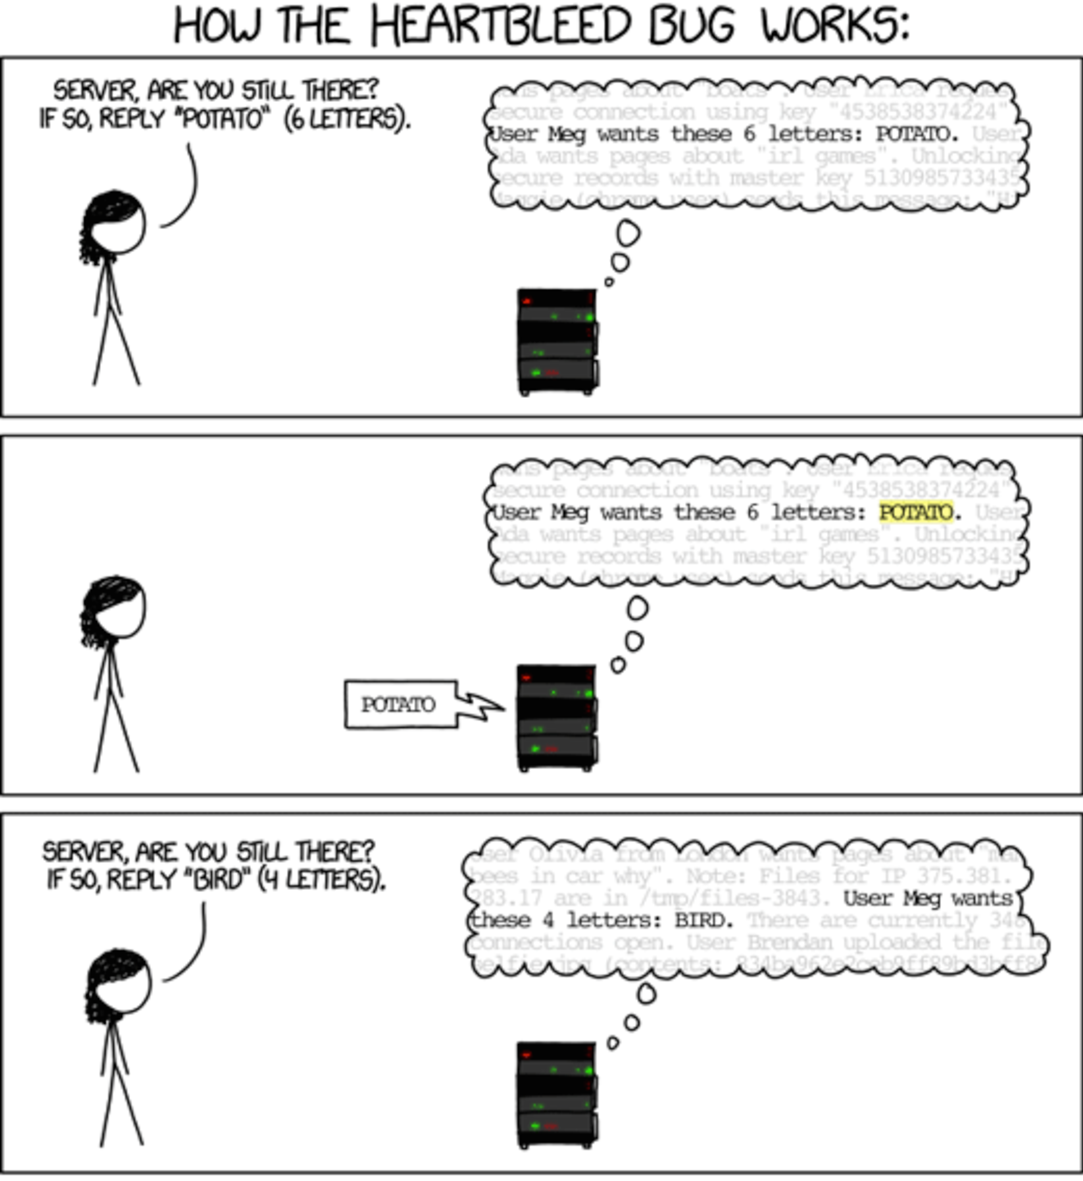
\includegraphics[width=50mm]{pic/heartbleed1} 
  \end{minipage}% 
  \begin{minipage}[t]{0.49\linewidth} 
    \centering 
    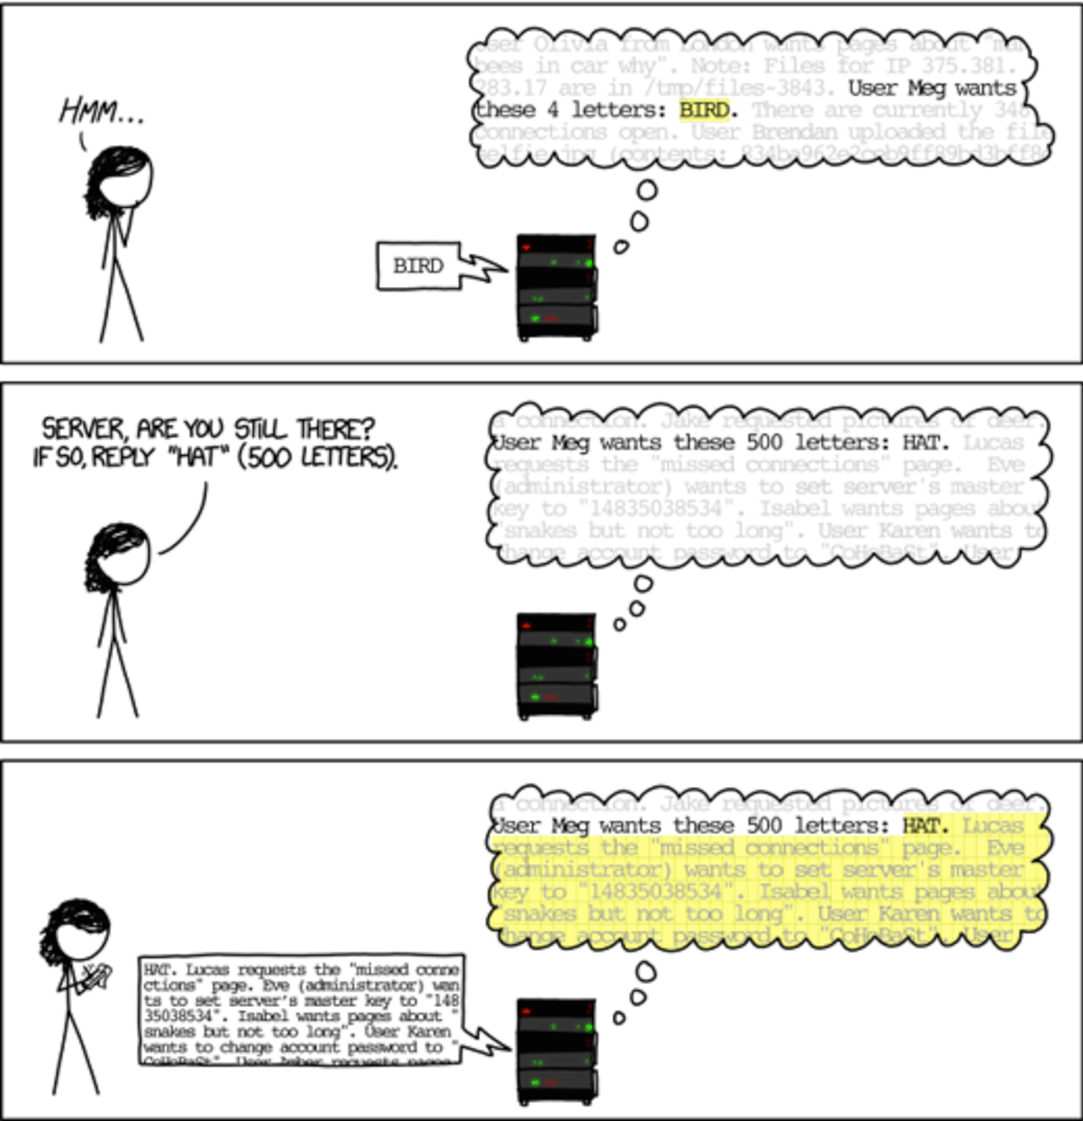
\includegraphics[width=50mm]{pic/heartbleed2} 
  \end{minipage}
\end{frame}
\begin{frame}\frametitle{Crypto is difficult to get right}
\begin{itemize}
\item Must be implemented correctly
\item Must be integrated from the beginning, not added on ``after the fact''
\item Need expertise; ``a little knowledge can be a dangerous thing''
\item Can't be secured by Q/A, only (at best) through penetration testing and dedicated review of the code by security experts
\end{itemize}
\end{frame}
\begin{frame}\frametitle{Beware of Snake Oil}
\textbf{Snake Oil}: bogus commercial cryptographic products.
\begin{itemize}
\item \textbf{Secret system}: security through obscurity
\item \textbf{Technobabble}: since cryptography is complicated
\item \textbf{Unbreakable}: a sure sign of snake oil
\item \textbf{One-time pads}: a flawed implementation
\item \textbf{Unsubstantiated ``bit'' claims}: key lengths are not directly comparable
\end{itemize}
\end{frame}
\begin{frame}\frametitle{General Recommendation}
\begin{itemize}
\item Use only standardized algorithms and protocols
\item No security through obscurity!
\item Use primitives for their intended purpose
\item Don't implement your own crypto
\item If your system cannot use ``off-the-shelf'' crypto components, re-think your system
\item If you really need something new, have it designed and/or evaluated by an expert
\item Don't use the same key for multiple purposes
\item Use good random-number generation
\end{itemize}
\end{frame}
\begin{frame}\frametitle{Crypto Libraries}
\begin{itemize}
\item Use existing, high-level crypto libraries: 
cryptlib, NaCl, Google's Keyczar, Mozilla's NSS, OpenSSL 
\item Avoid low-level libraries (like JCE, crypto++, GnuPG, OpenPGP) - too much possibility of mis-use
\item Avoid writing your own low-level crypto
\end{itemize}
\end{frame}
\end{document}
